% 
% mH=125 GeV, 1-jet
% 
\begin{figure}[htp]
\centering
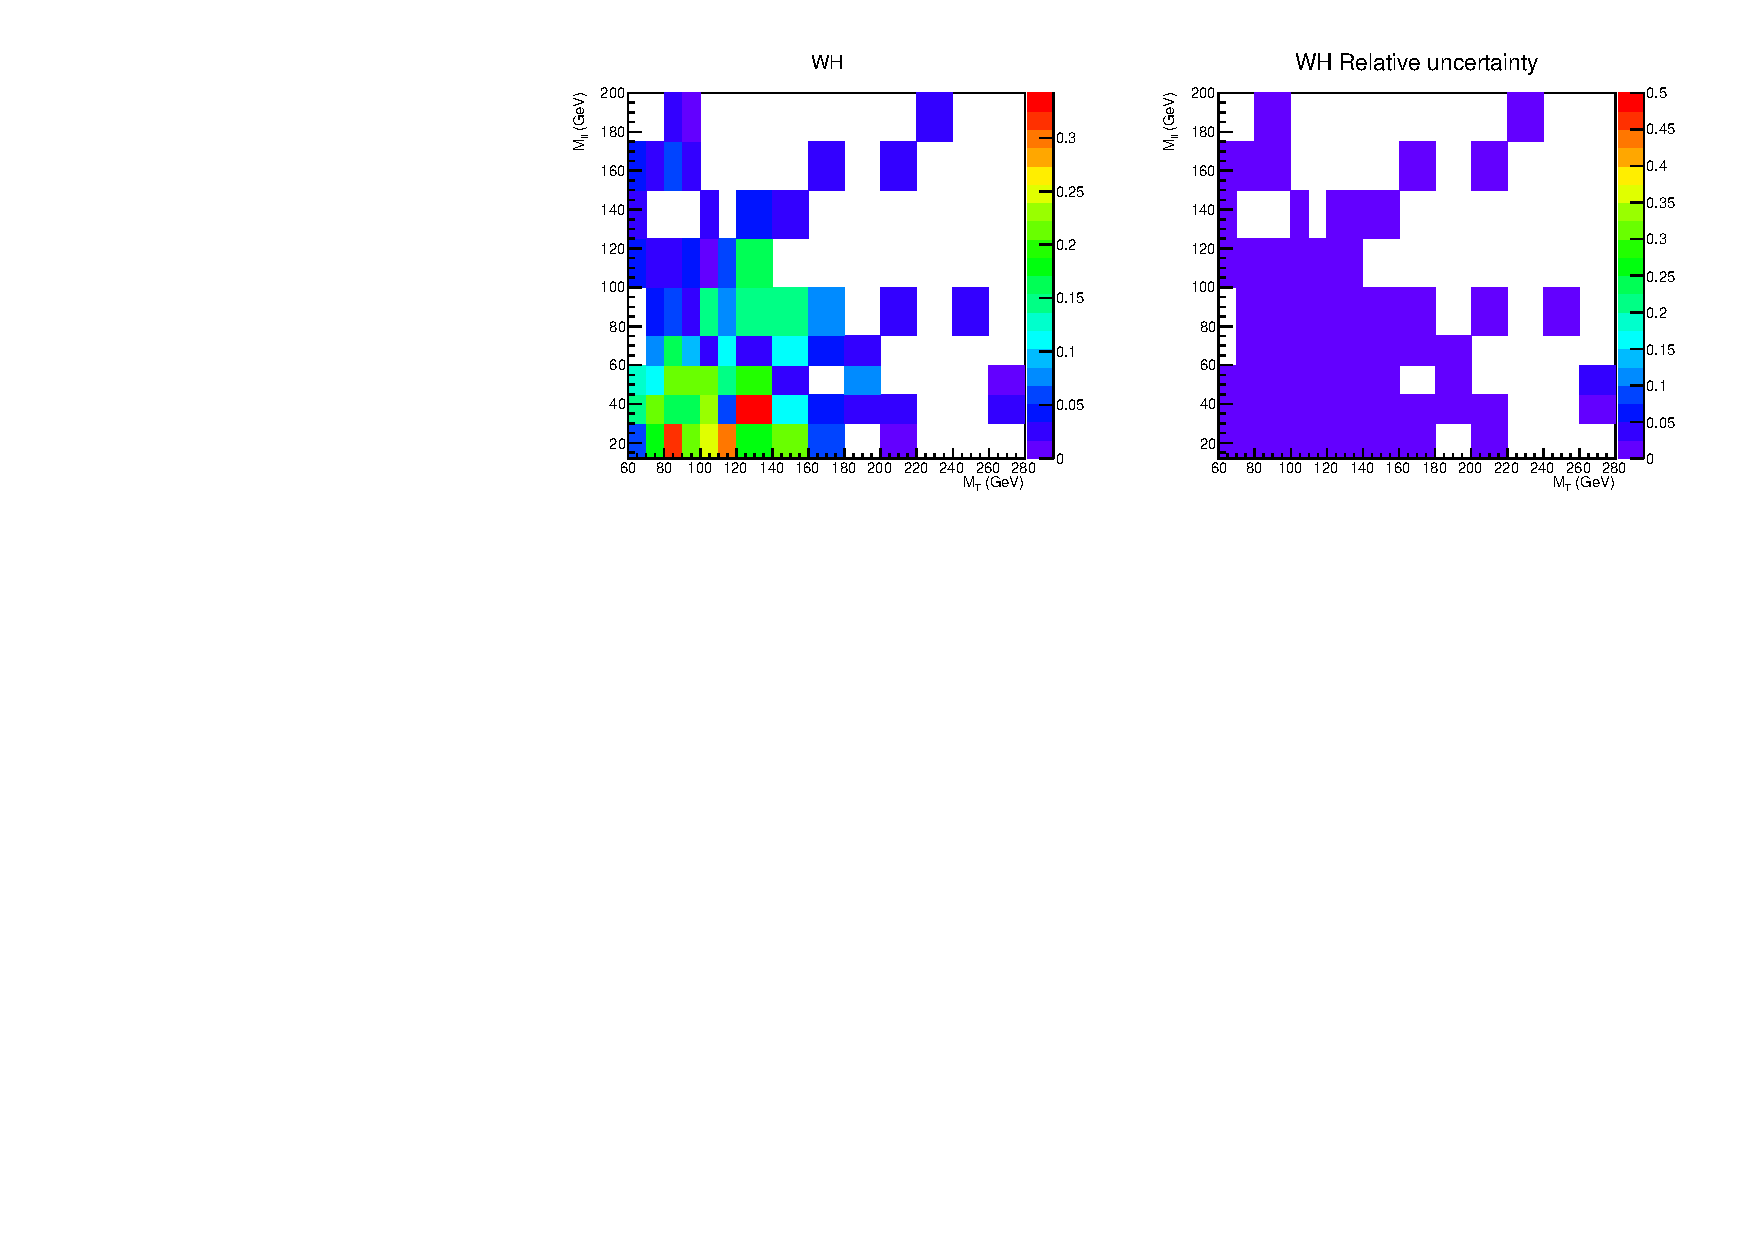
\includegraphics[width=0.8\textwidth]{figures/2dtemplate_WH_mH125_1j.pdf}
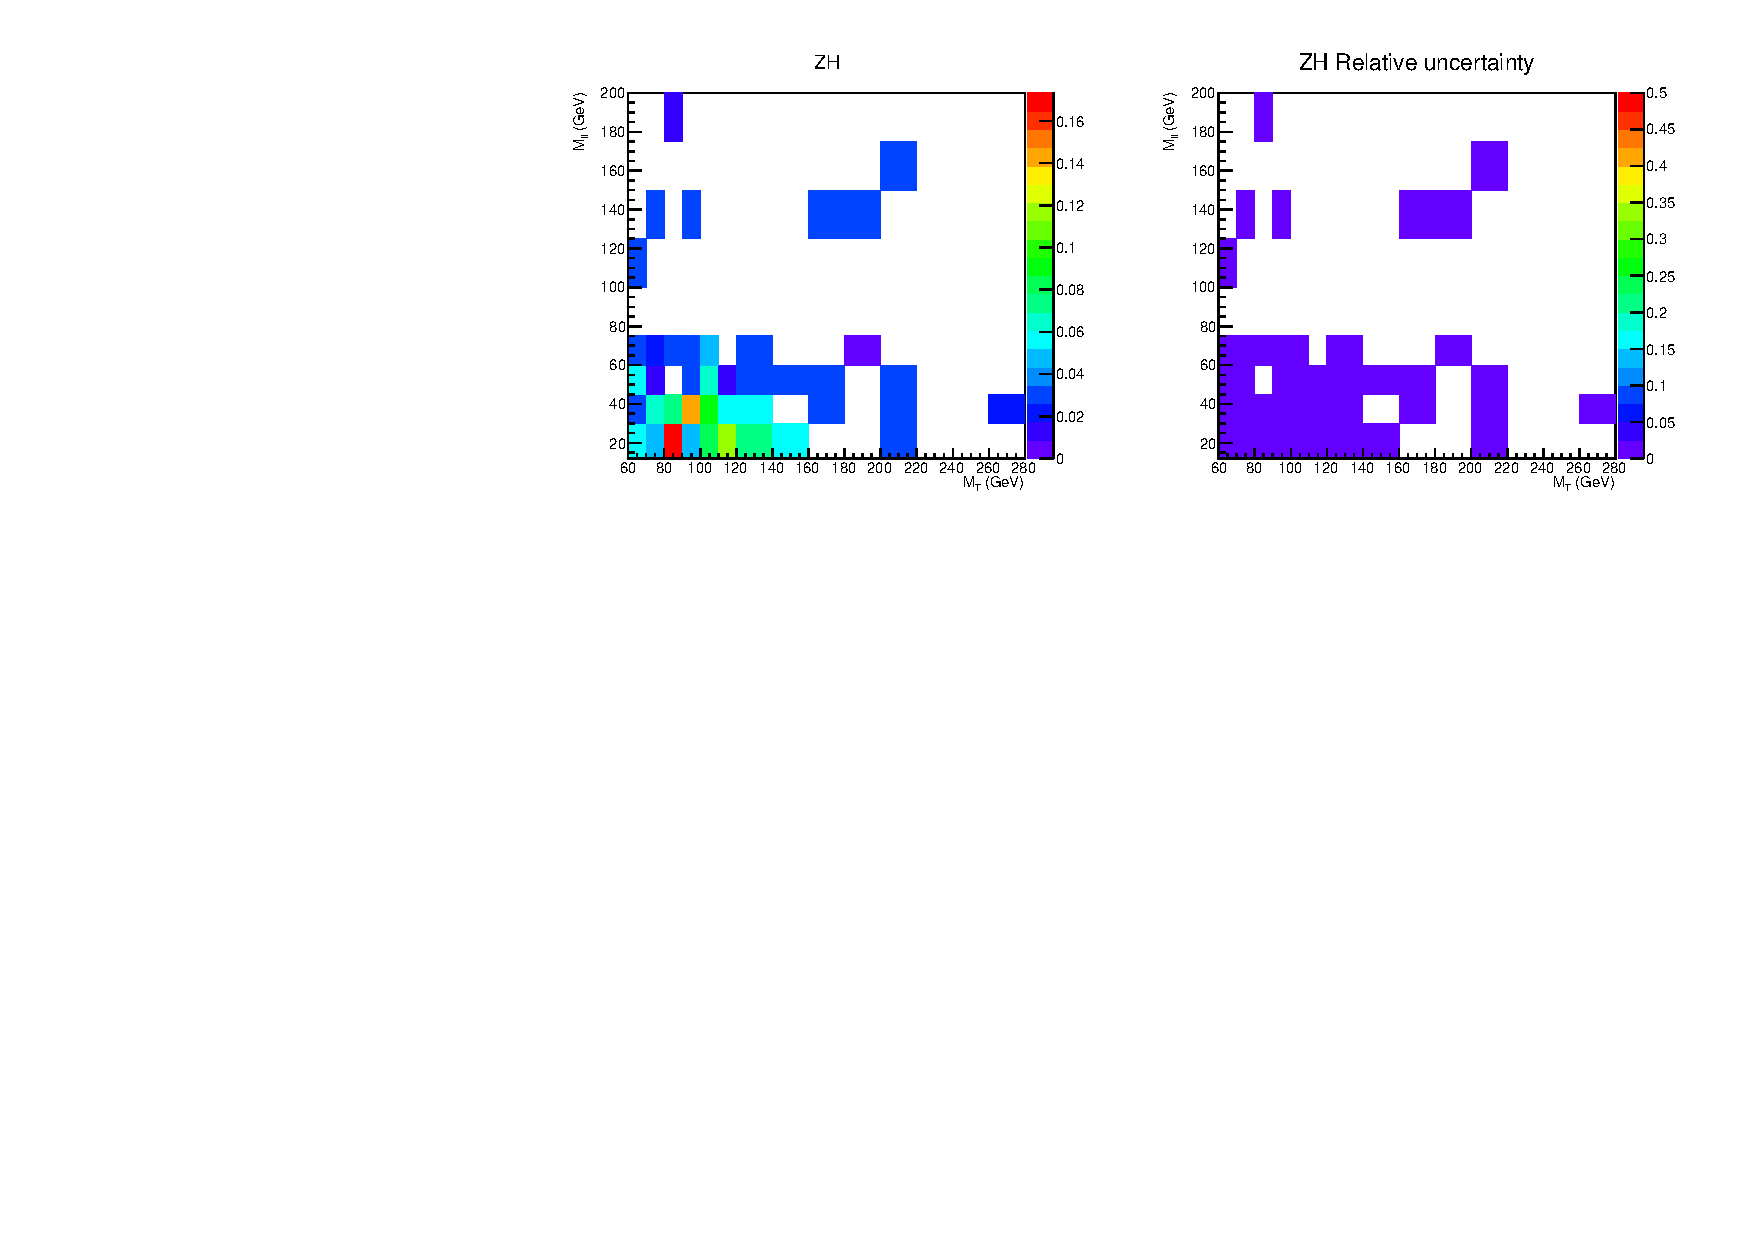
\includegraphics[width=0.8\textwidth]{figures/2dtemplate_ZH_mH125_1j.pdf}
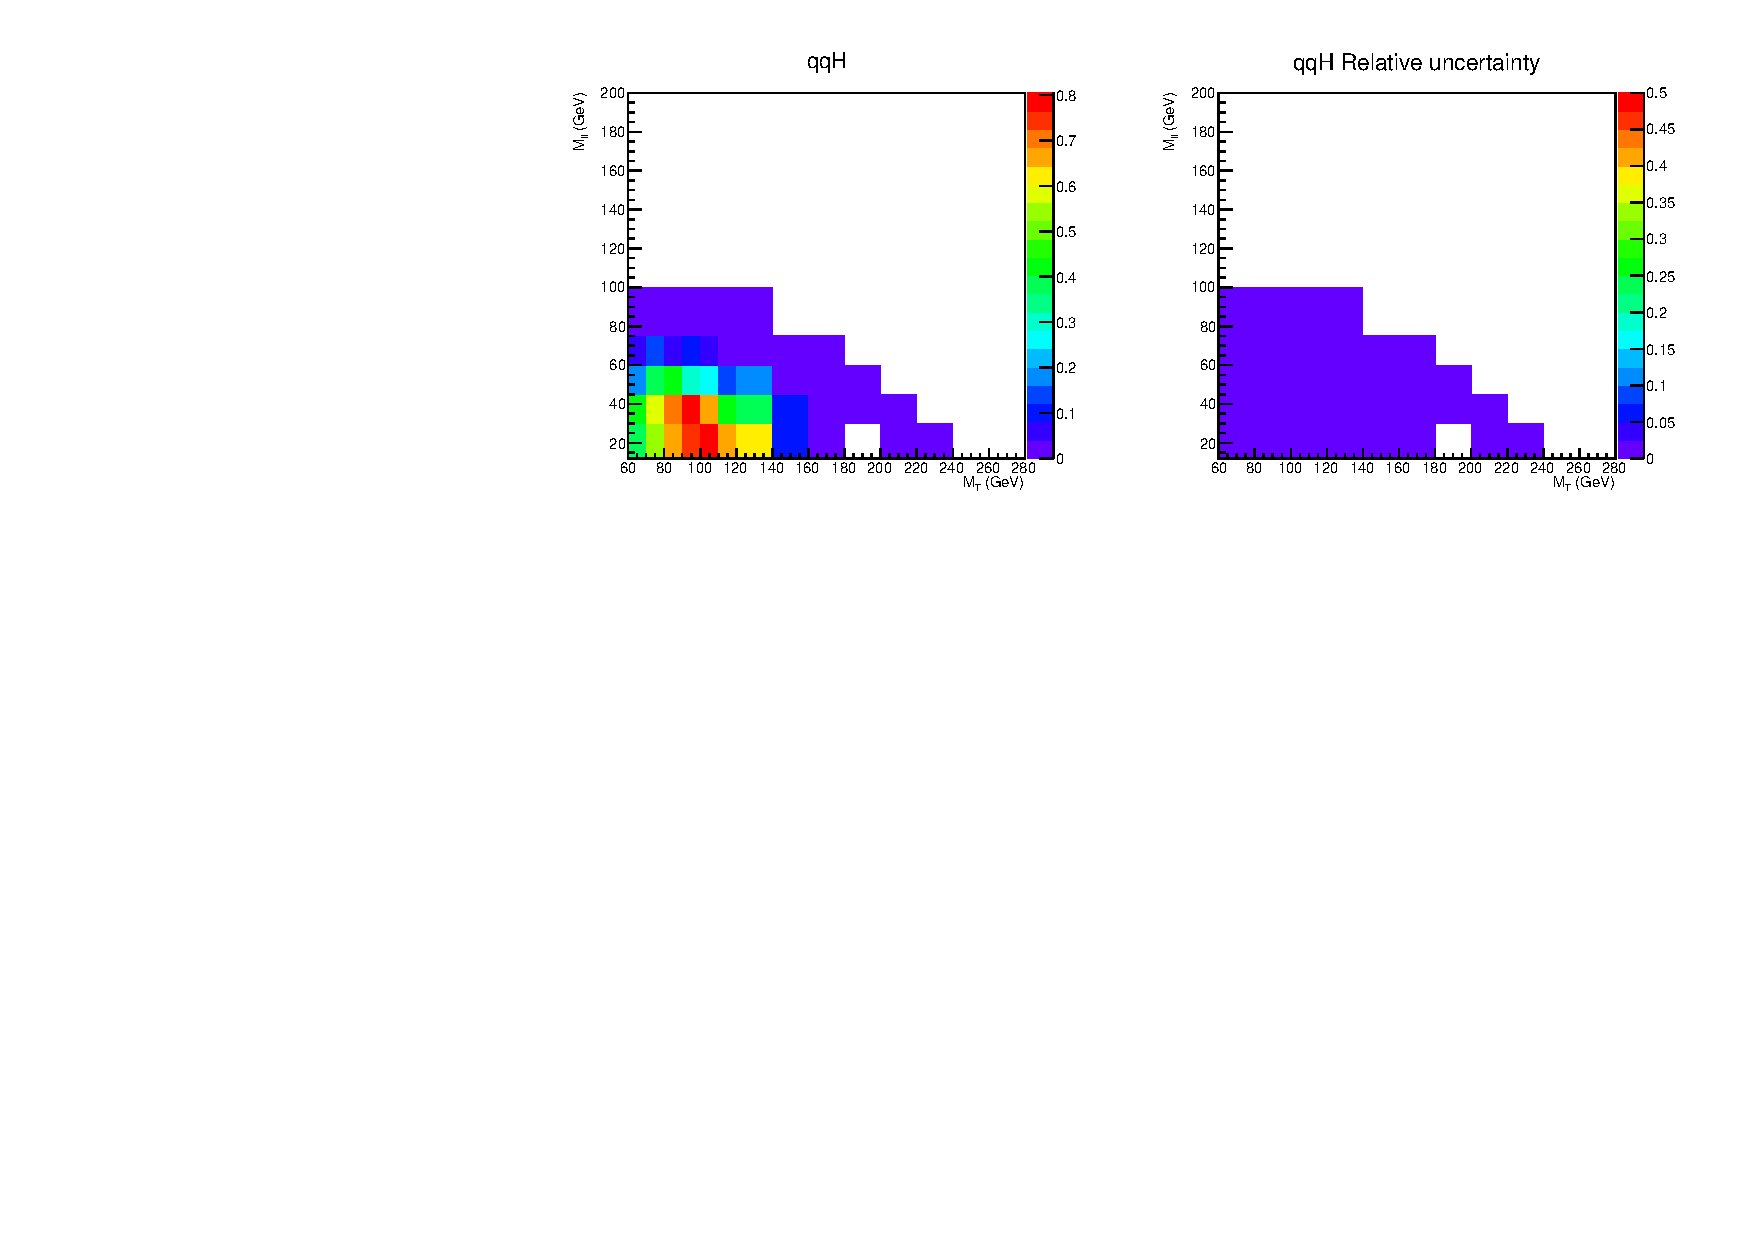
\includegraphics[width=0.8\textwidth]{figures/2dtemplate_qqH_mH125_1j.pdf}
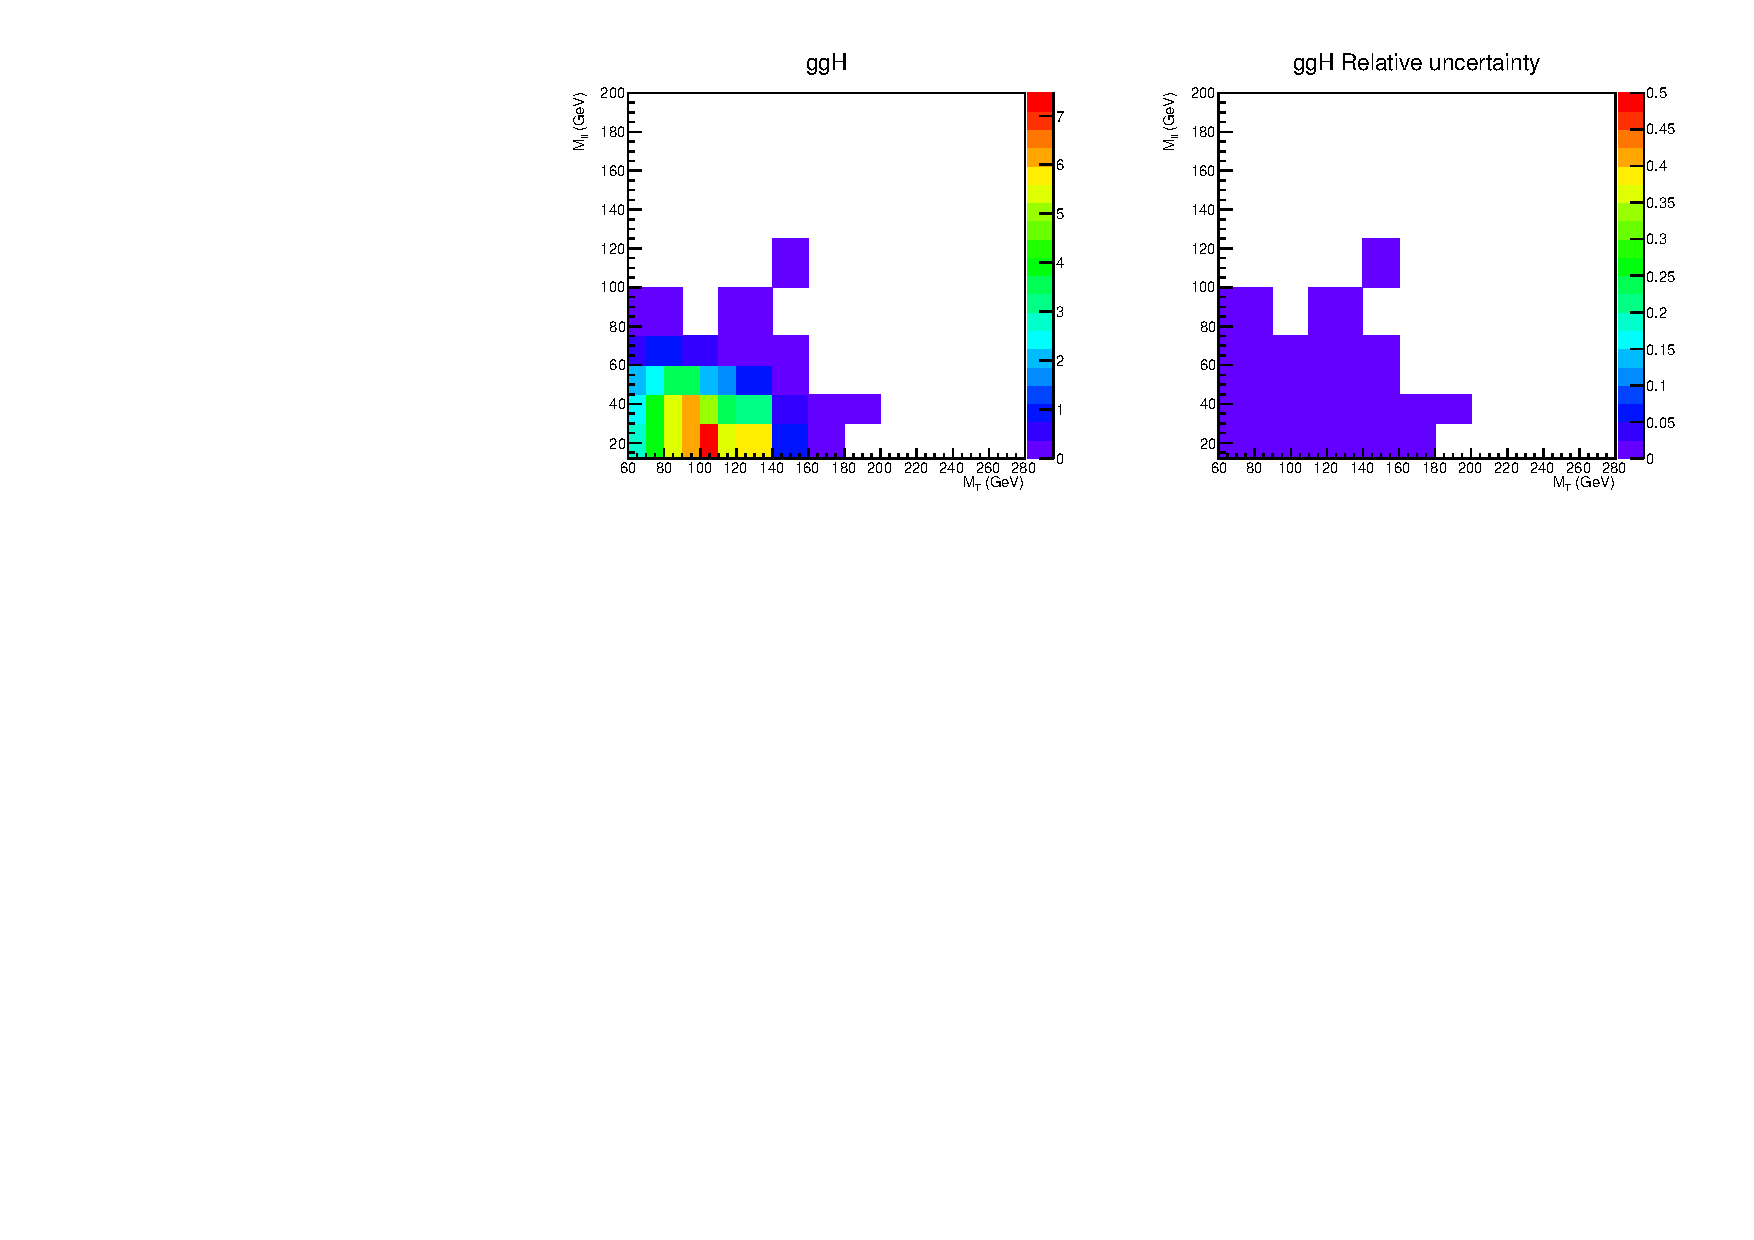
\includegraphics[width=0.8\textwidth]{figures/2dtemplate_ggH_mH125_1j.pdf}
\caption{Templates(left) and relative statistical uncertainty of the MC sample(right) 
of \qqWH, \qqZH, \qqH\ and \ggH. 
The templates are for \mHi\ = 125 \GeV\ analysis in the 1-jet category.}
\label{fig:2dtemplate_125_1j_1}
\end{figure}

\begin{figure}[htp]
\centering
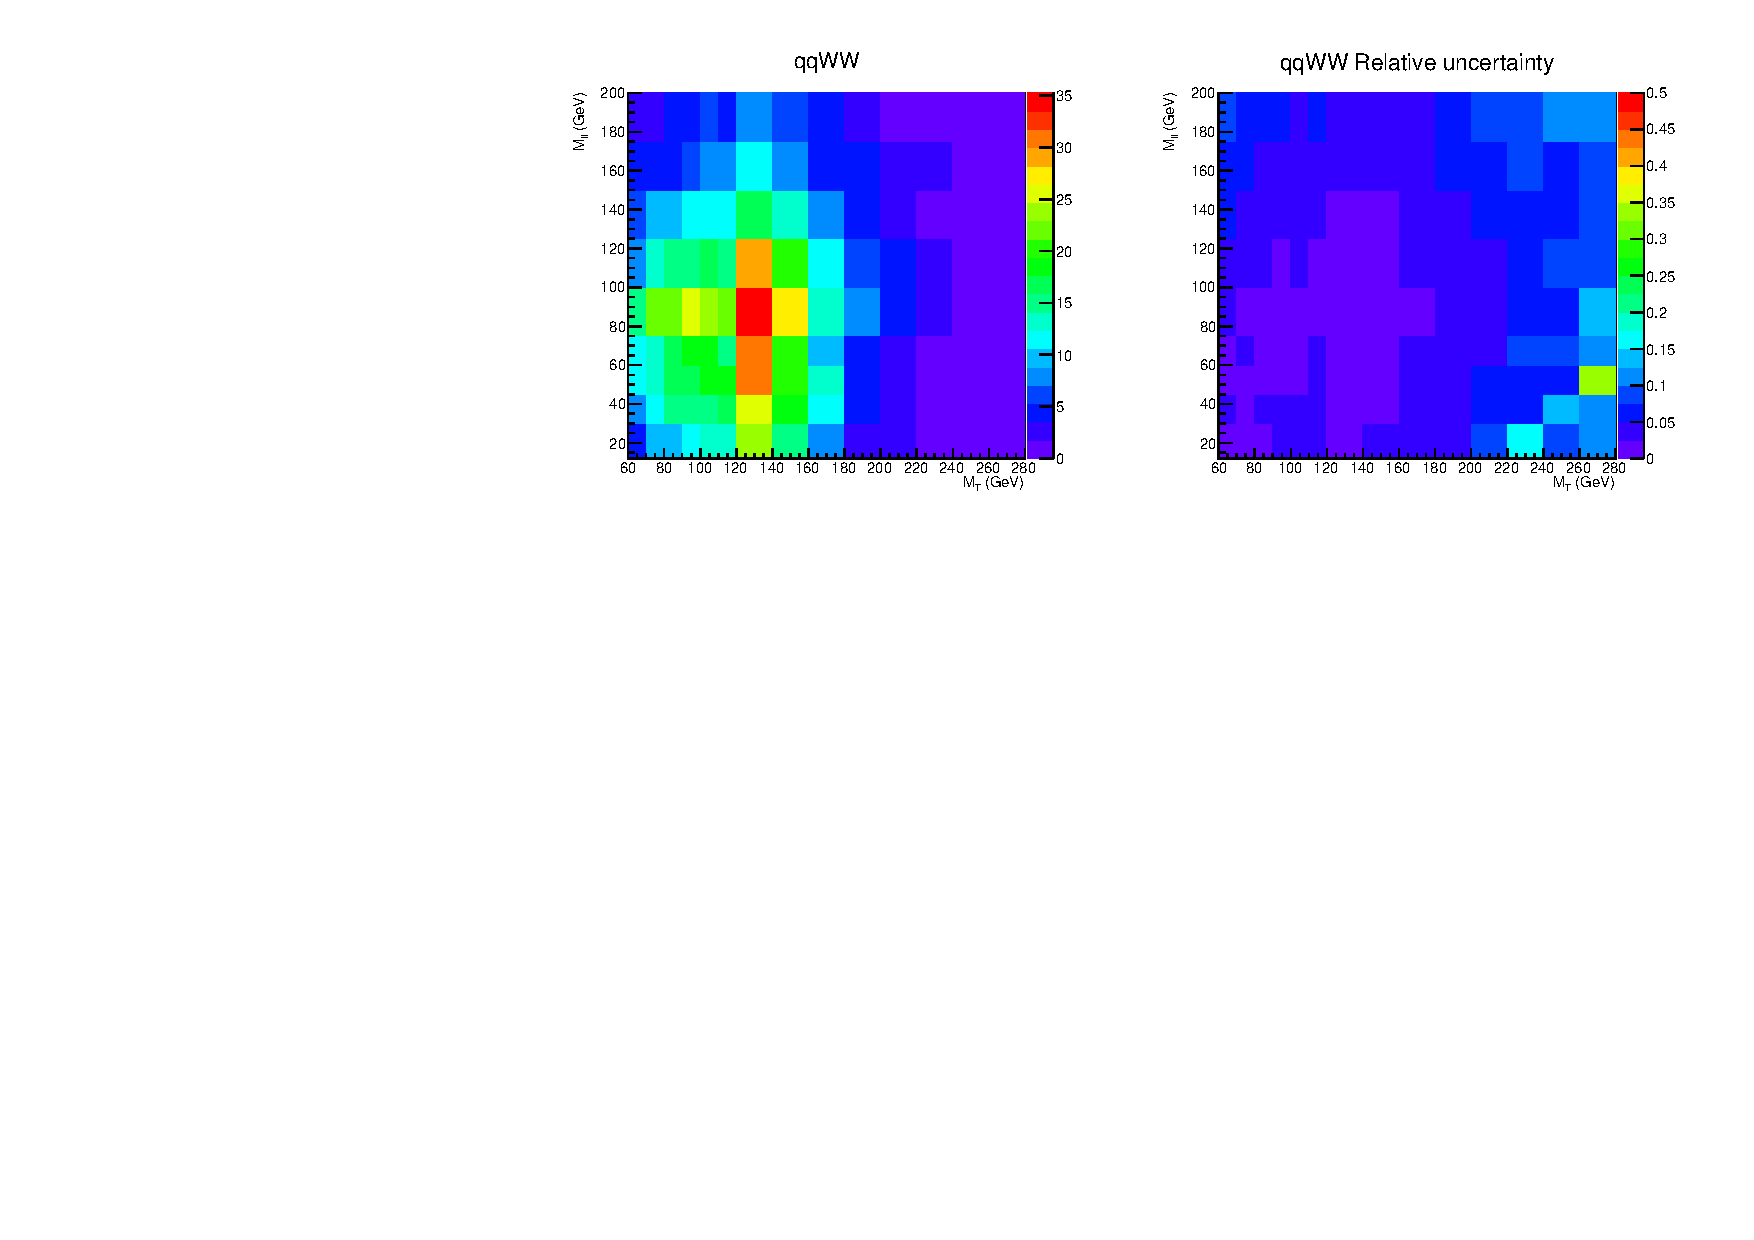
\includegraphics[width=0.8\textwidth]{figures/2dtemplate_qqWW_mH125_1j.pdf}
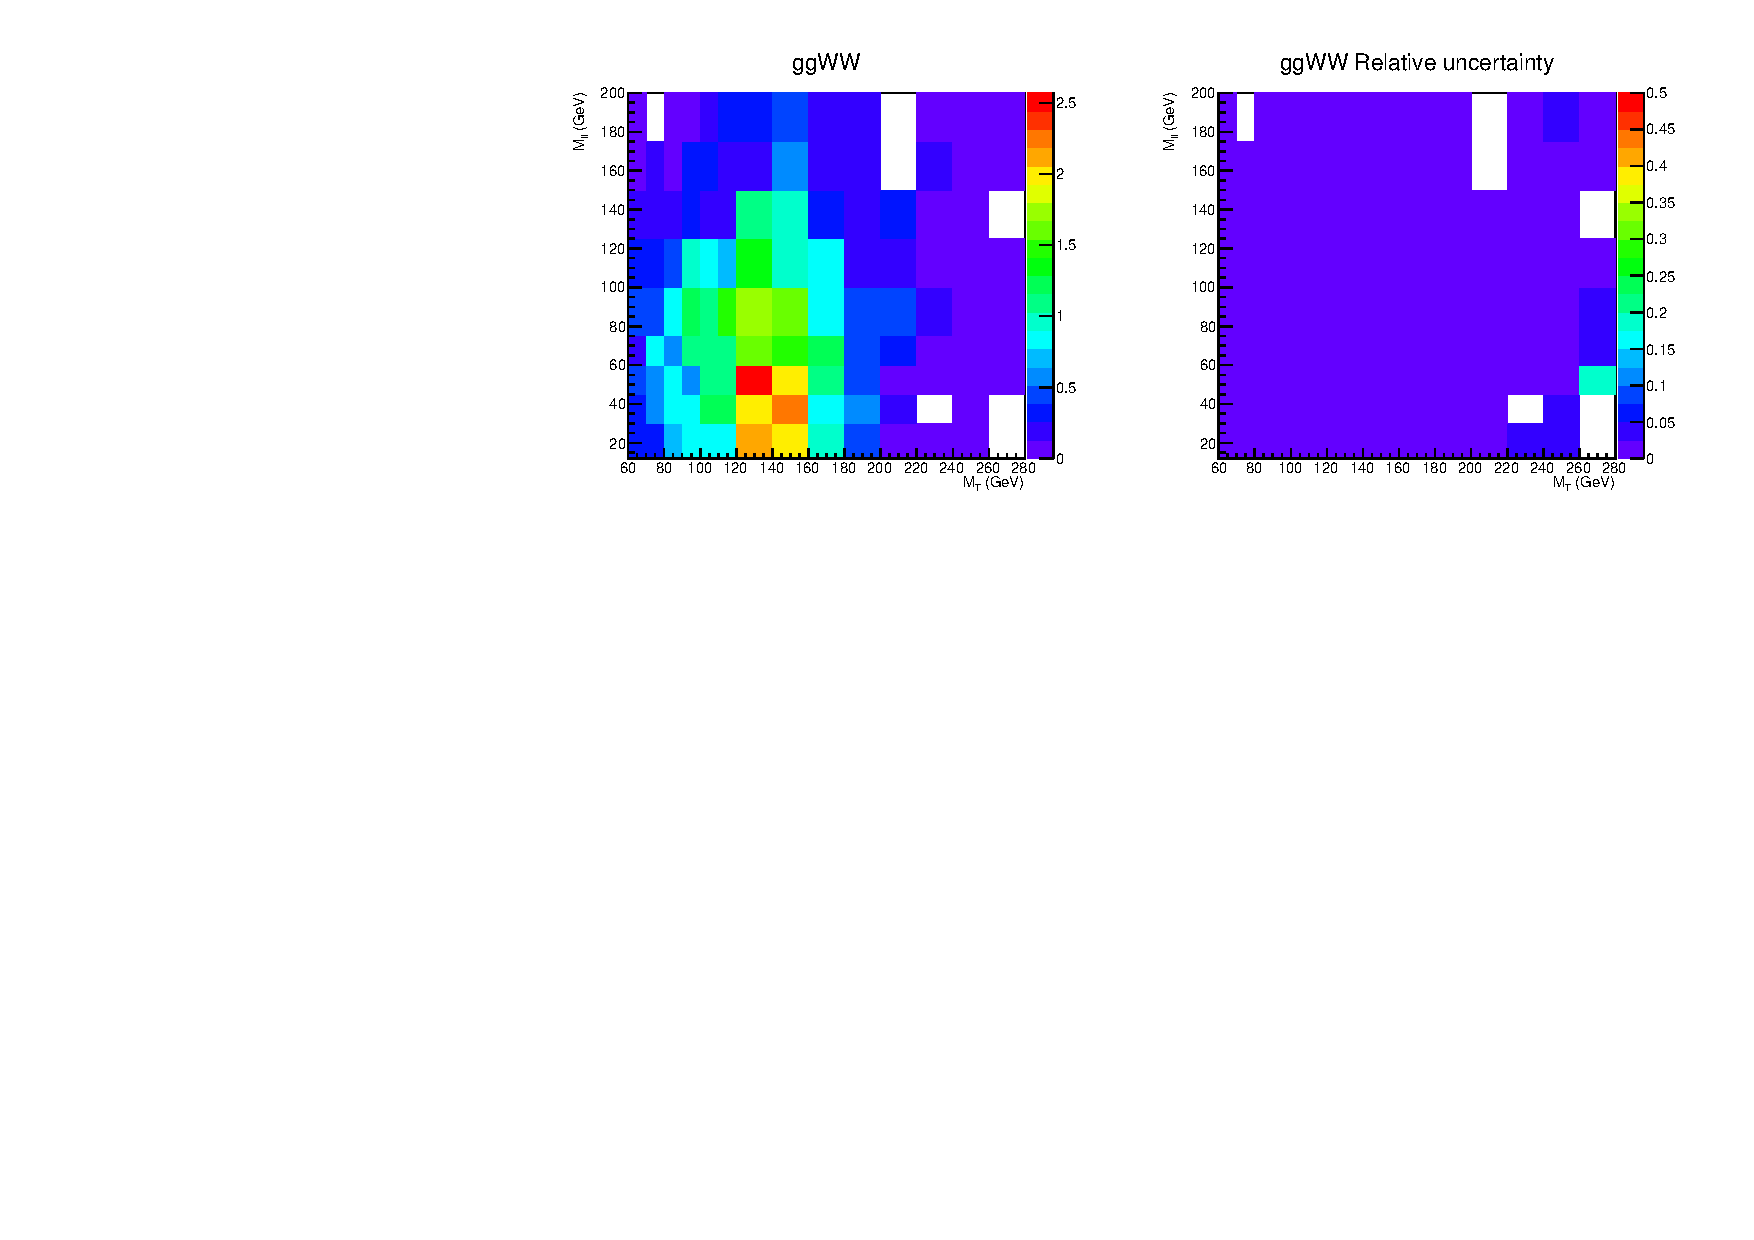
\includegraphics[width=0.8\textwidth]{figures/2dtemplate_ggWW_mH125_1j.pdf}
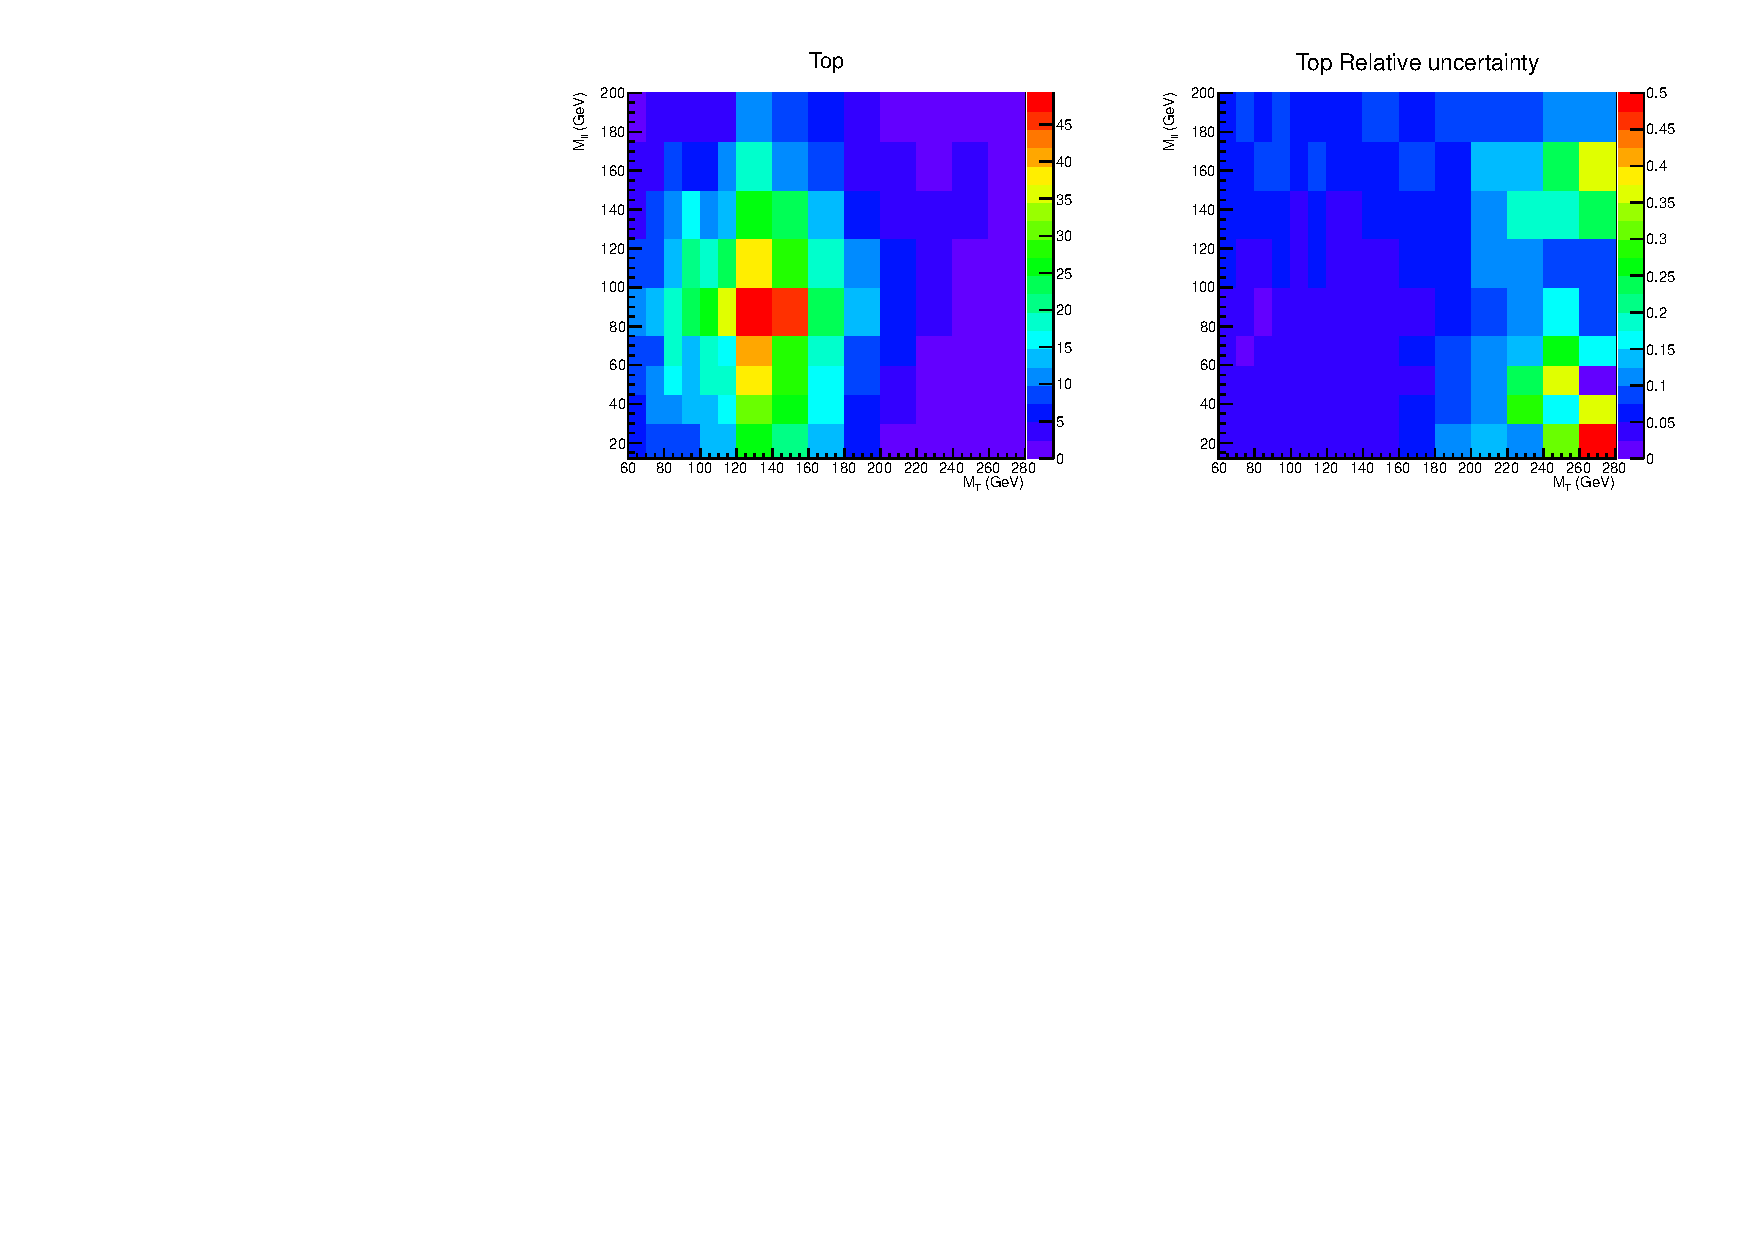
\includegraphics[width=0.8\textwidth]{figures/2dtemplate_Top_mH125_1j.pdf}
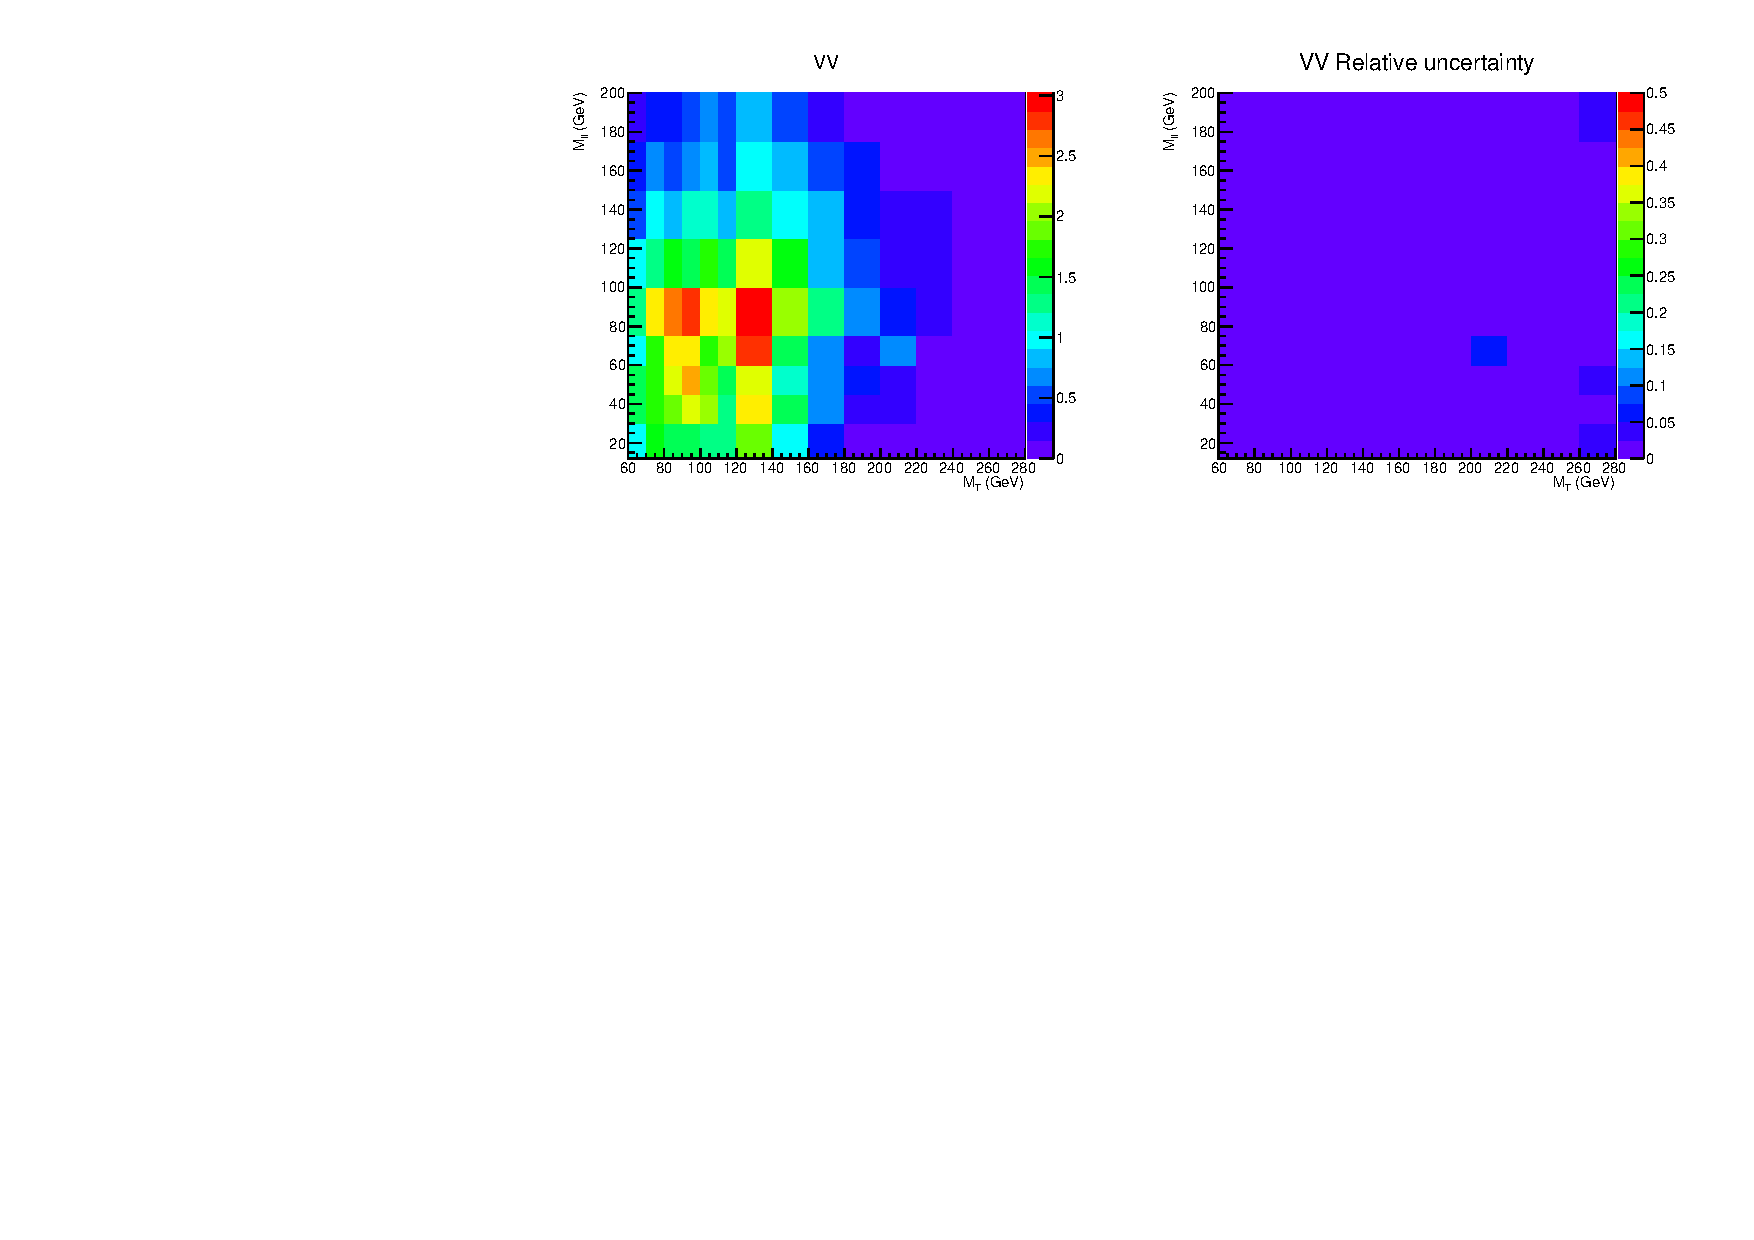
\includegraphics[width=0.8\textwidth]{figures/2dtemplate_VV_mH125_1j.pdf}
\caption{Templates(left) and relative statistical uncertainty of the MC sample(right) 
of \qqww, \ggww, \topbkg\ and \vv. 
The templates are for \mHi\ = 125 \GeV\ analysis in the 1-jet category.}
\label{fig:2dtemplate_125_1j_2}
\end{figure}

\begin{figure}[htp]
\centering
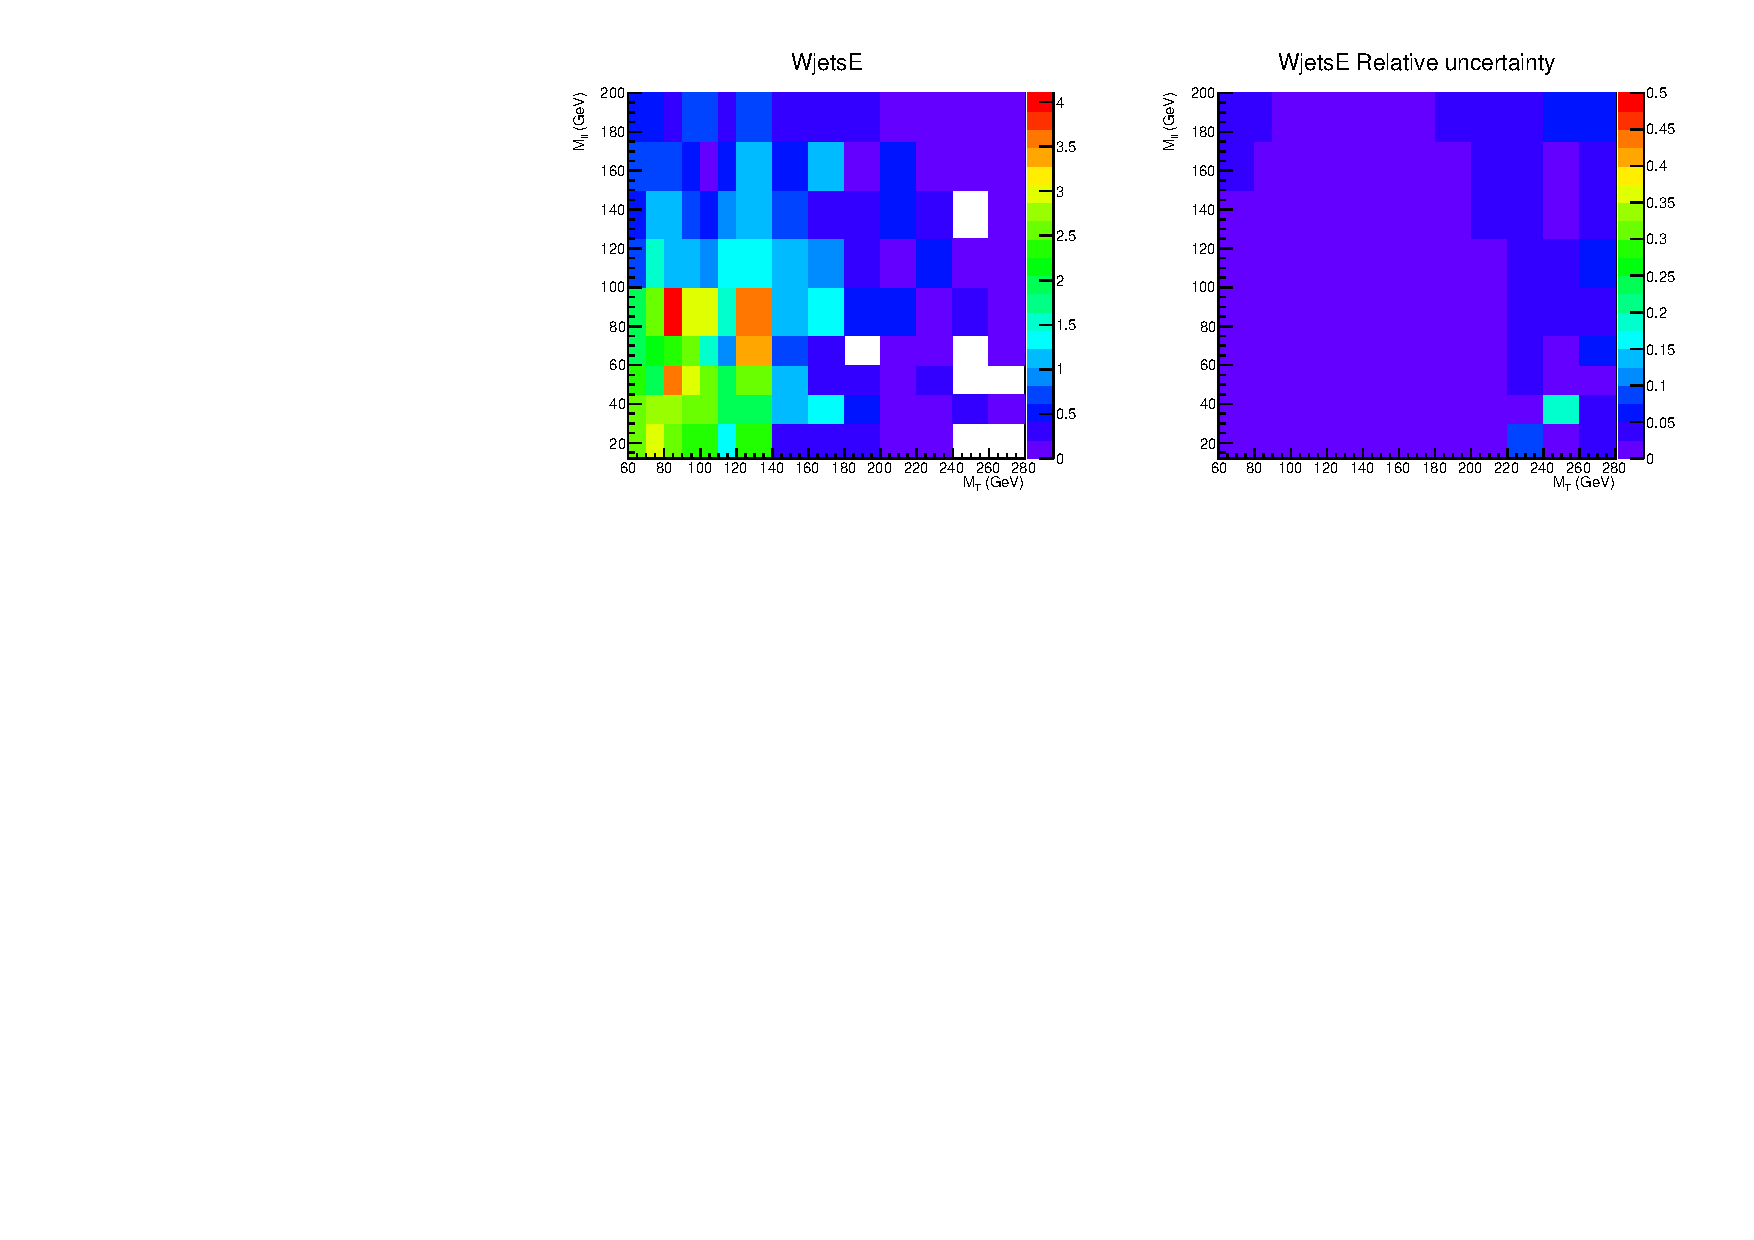
\includegraphics[width=0.8\textwidth]{figures/2dtemplate_WjetsE_mH125_1j.pdf}
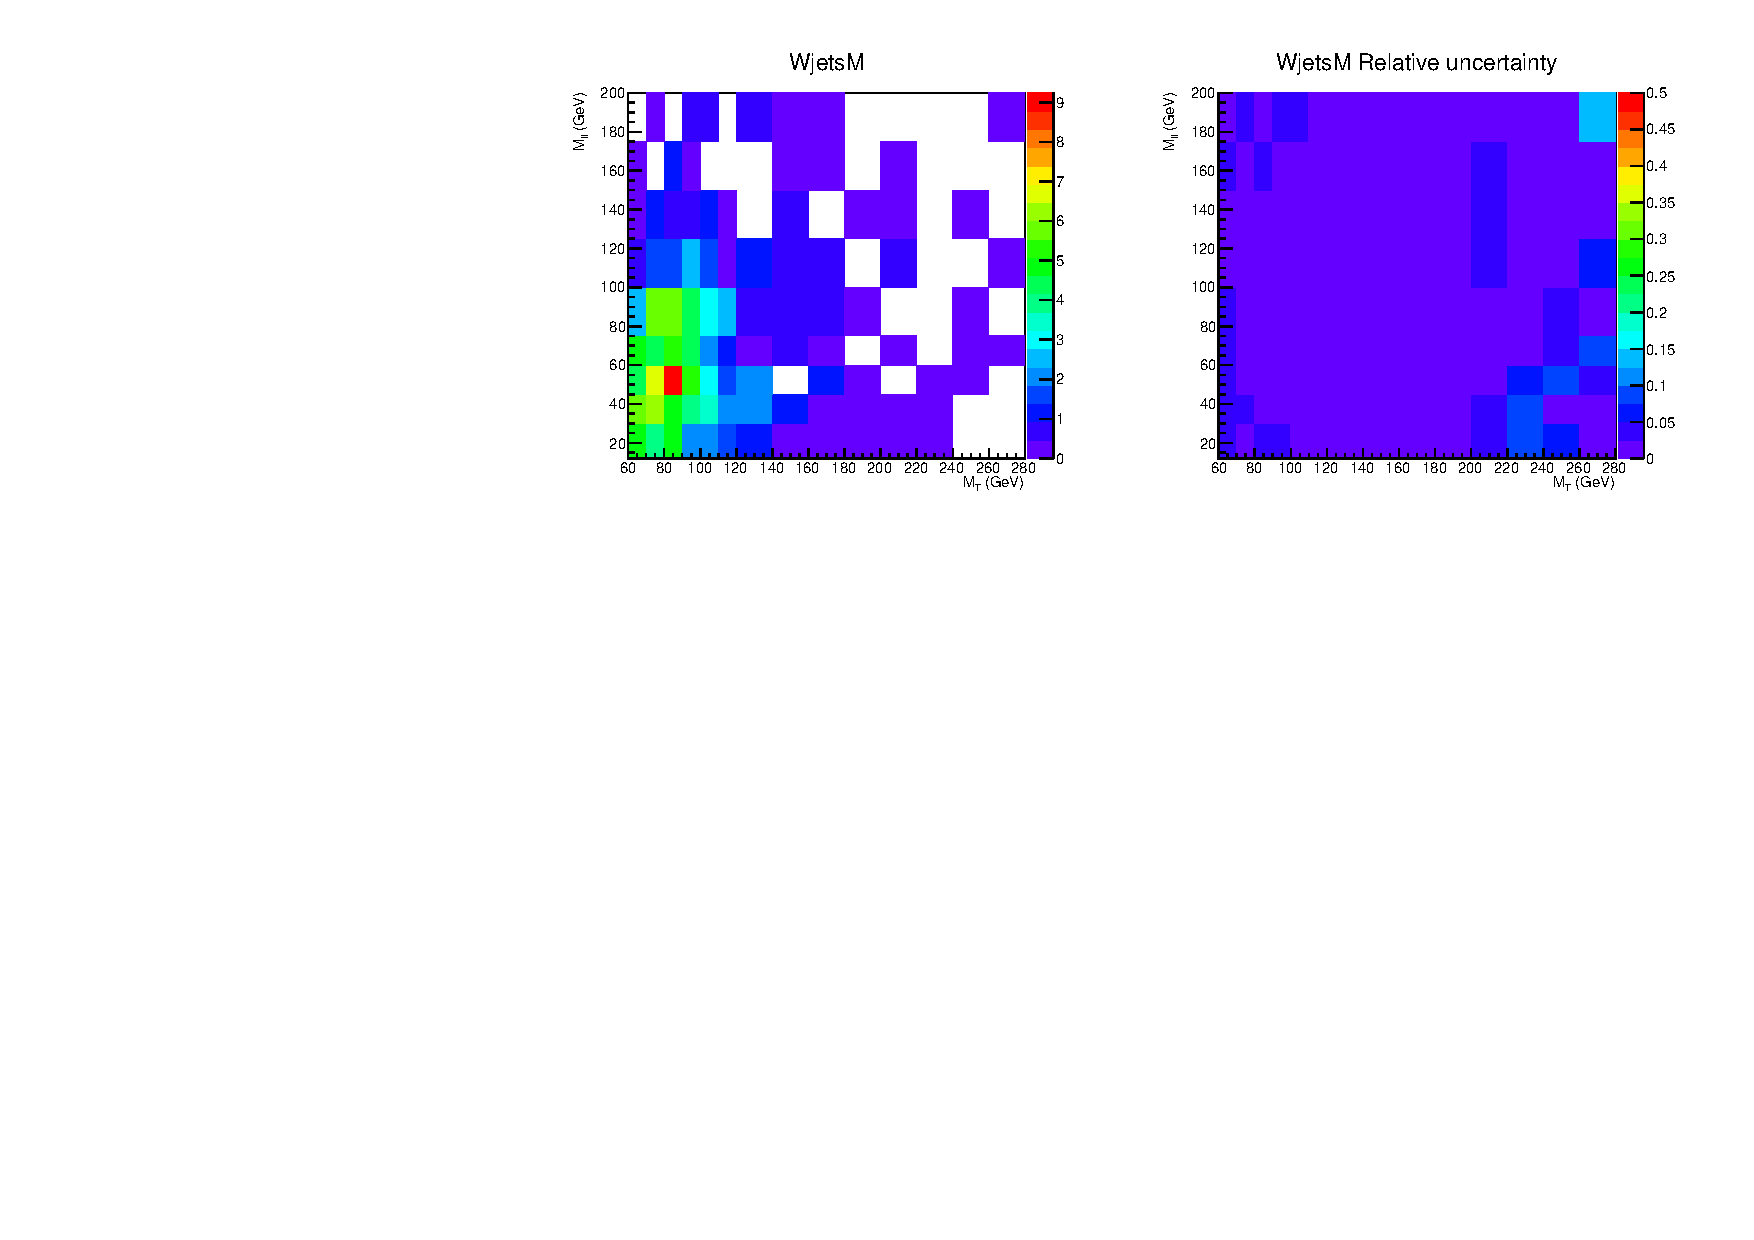
\includegraphics[width=0.8\textwidth]{figures/2dtemplate_WjetsM_mH125_1j.pdf}
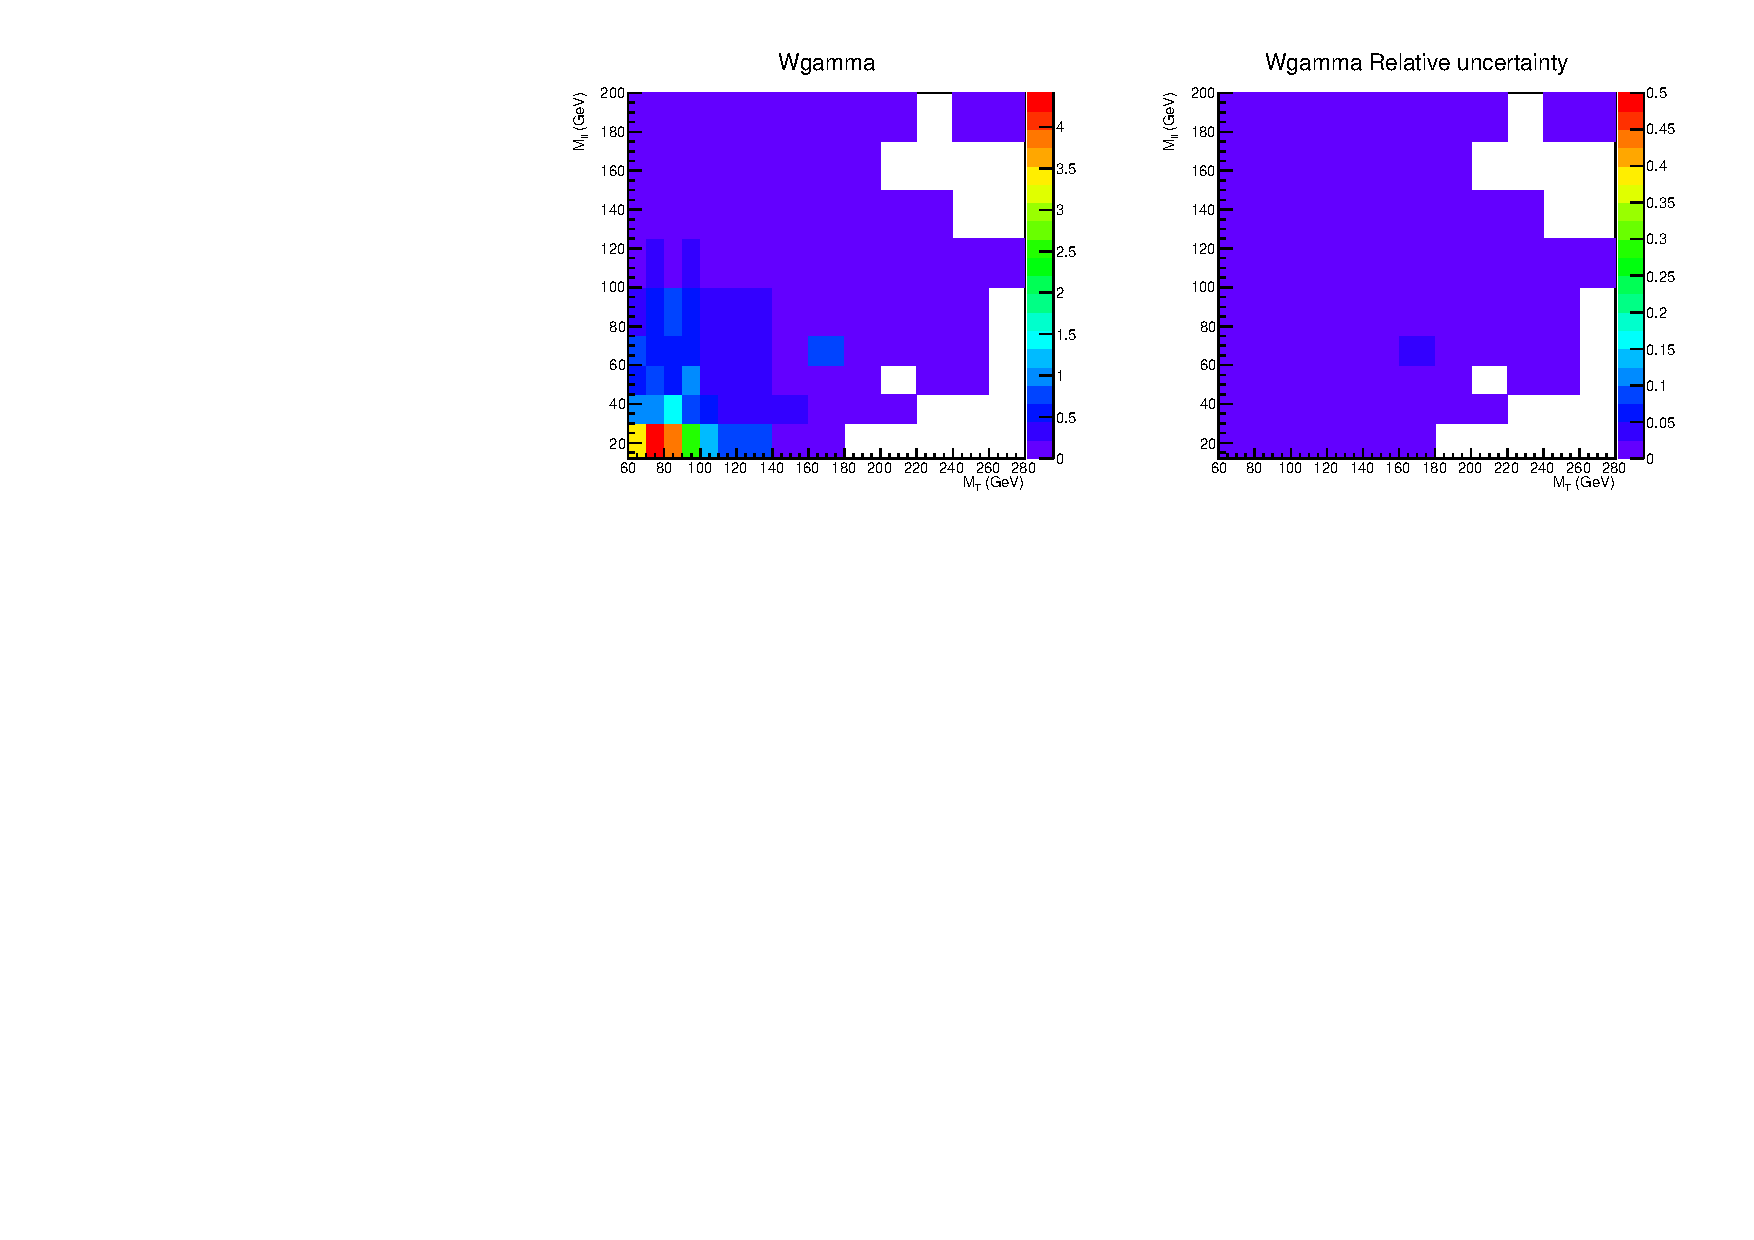
\includegraphics[width=0.8\textwidth]{figures/2dtemplate_Wgamma_mH125_1j.pdf}
\caption{Templates(left) and relative statistical uncertainty of the MC sample(right) 
of \WjetsE, \WjetsM\ and \wgamma. 
The templates are for \mHi\ = 125 \GeV\ analysis in the 1-jet category.}
\label{fig:2dtemplate_125_1j_3}
\end{figure}

\begin{figure}[htp]
\centering
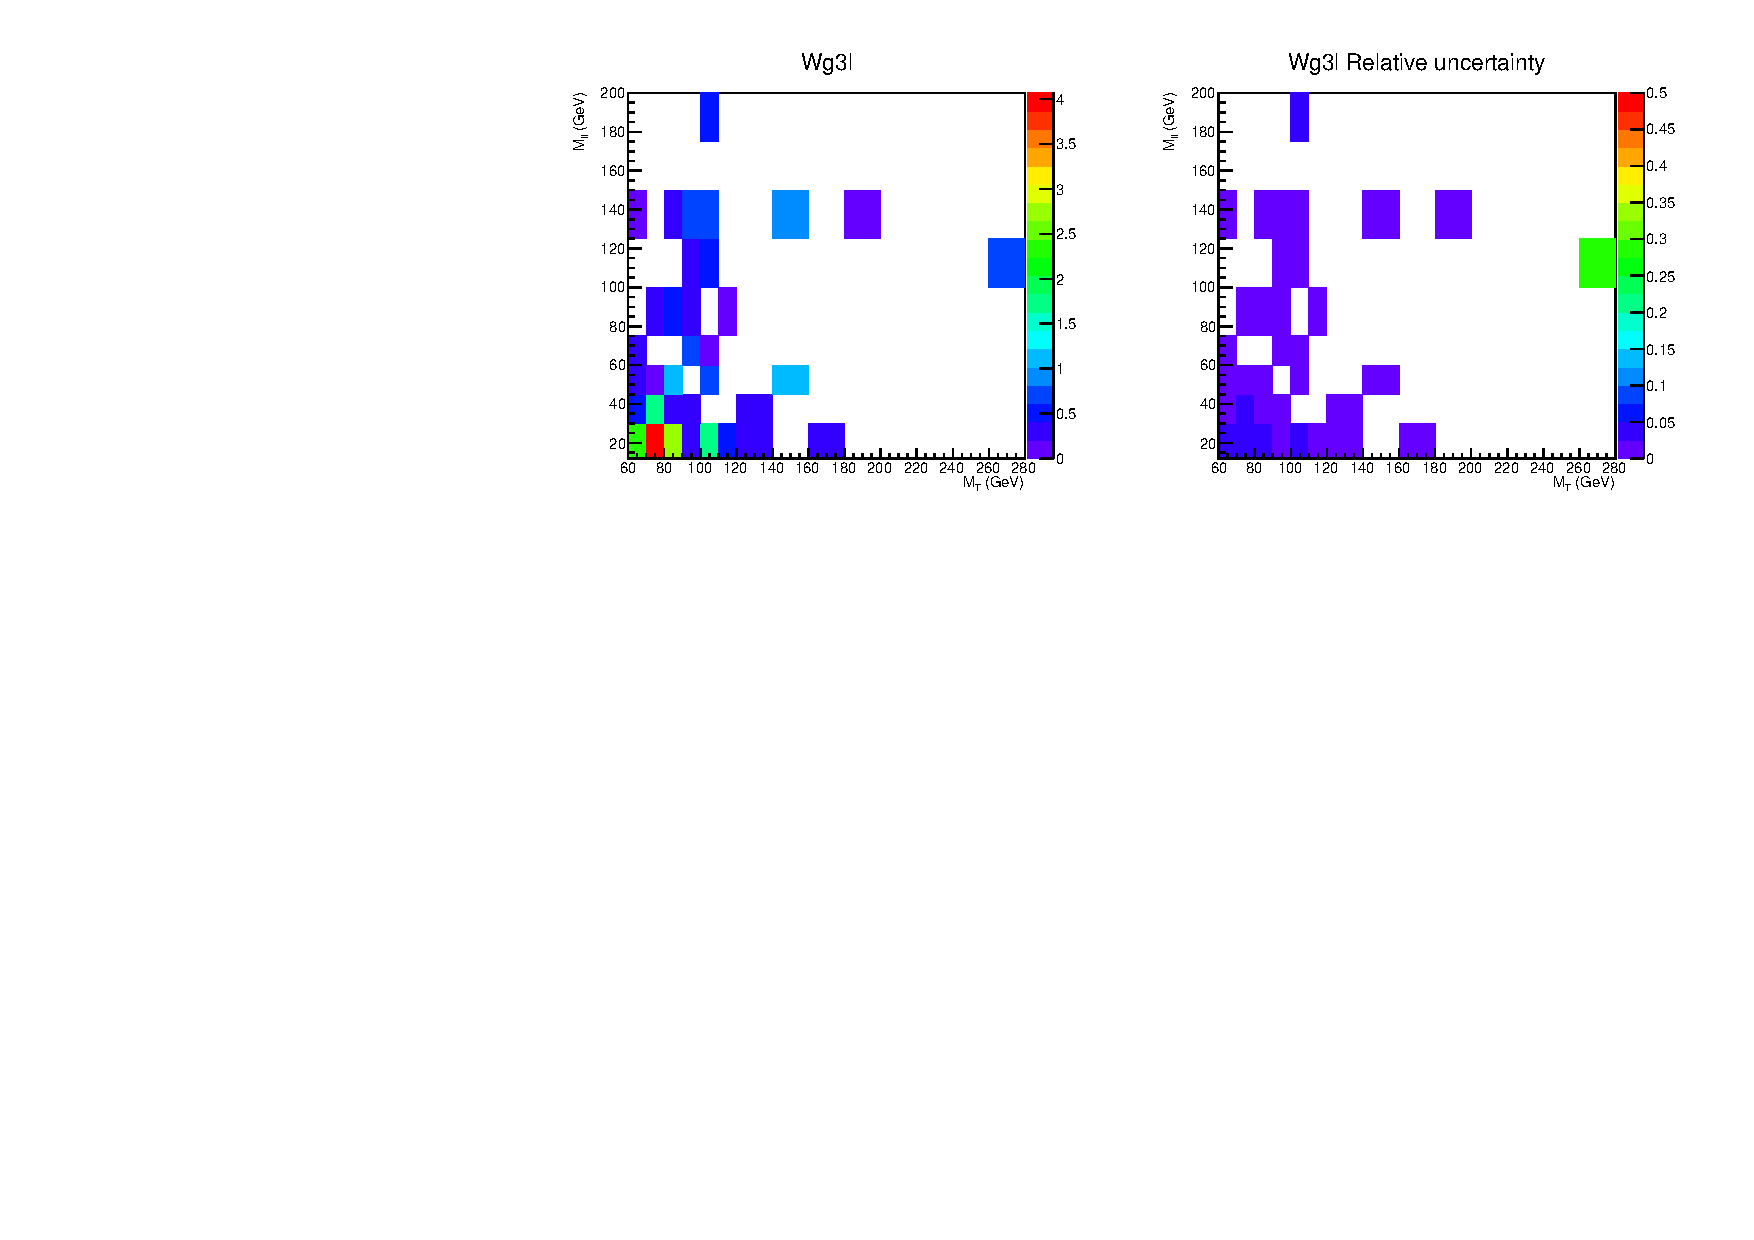
\includegraphics[width=0.8\textwidth]{figures/2dtemplate_Wg3l_mH125_1j.pdf}
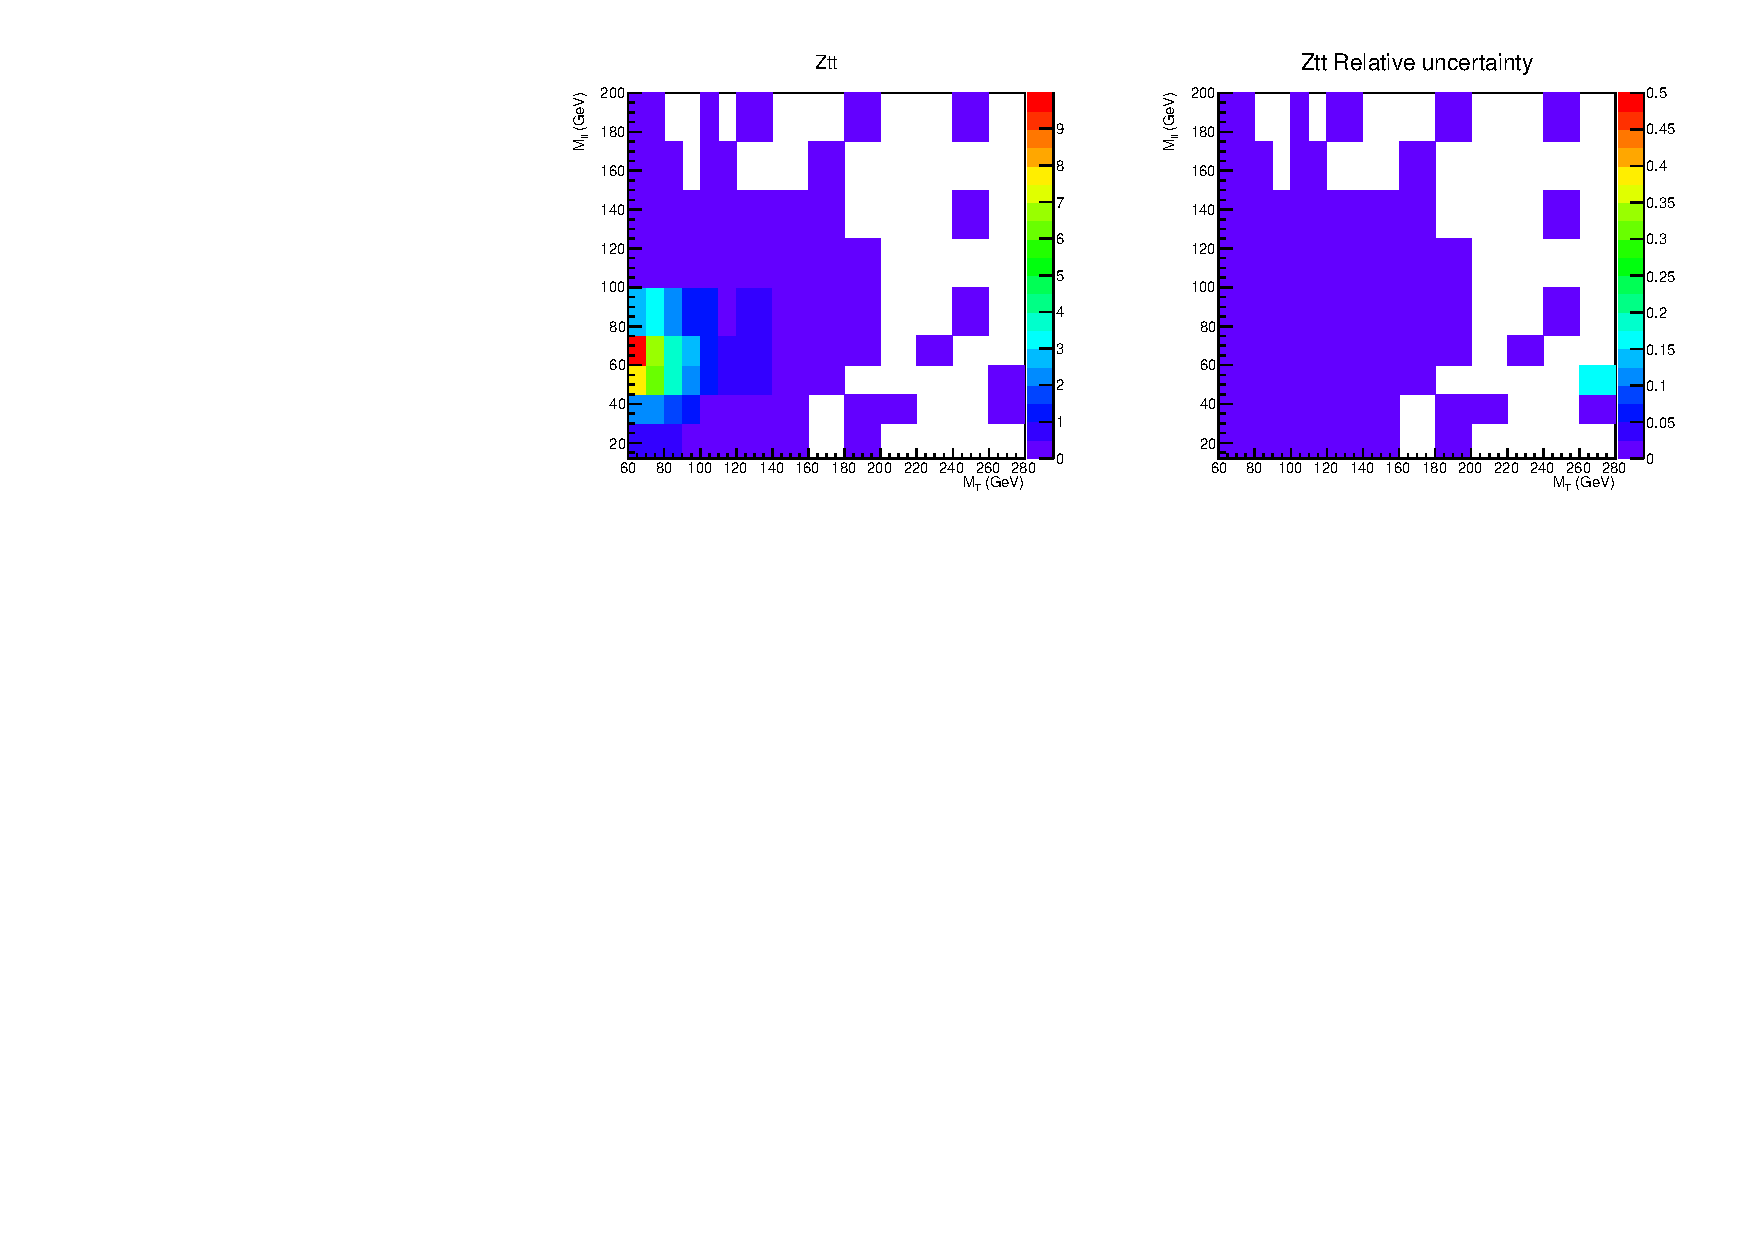
\includegraphics[width=0.8\textwidth]{figures/2dtemplate_Ztt_mH125_1j.pdf}
\caption{Templates(left) and relative statistical uncertainty of the MC sample(right) 
of \wgammastar\ and \ztt. 
The templates are for \mHi\ = 125 \GeV\ analysis in the 1-jet category.}
\label{fig:2dtemplate_125_1j_4}
\end{figure} 


% 
% mH=400 GeV, 0-jet
% 
\begin{figure}[htp]
\centering
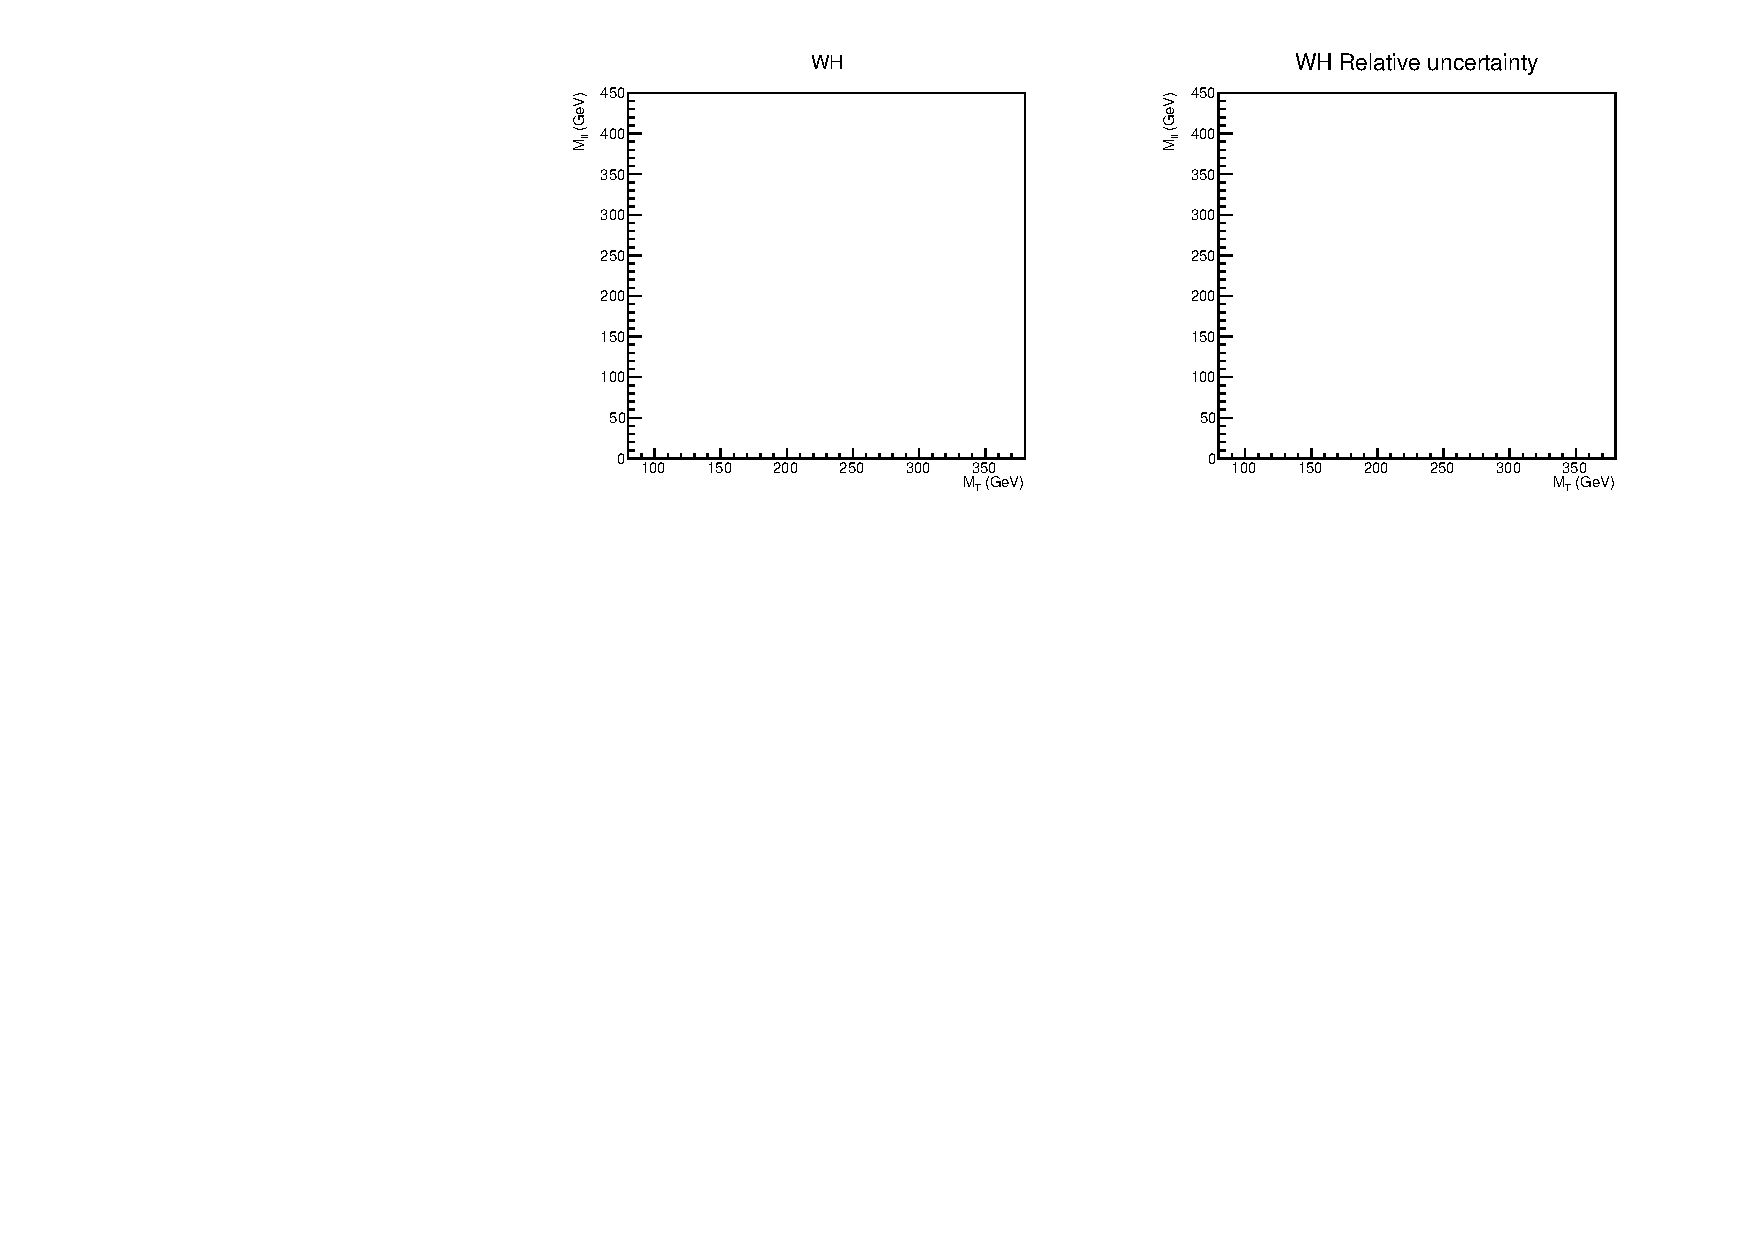
\includegraphics[width=0.8\textwidth]{figures/2dtemplate_WH_mH400_0j.pdf}
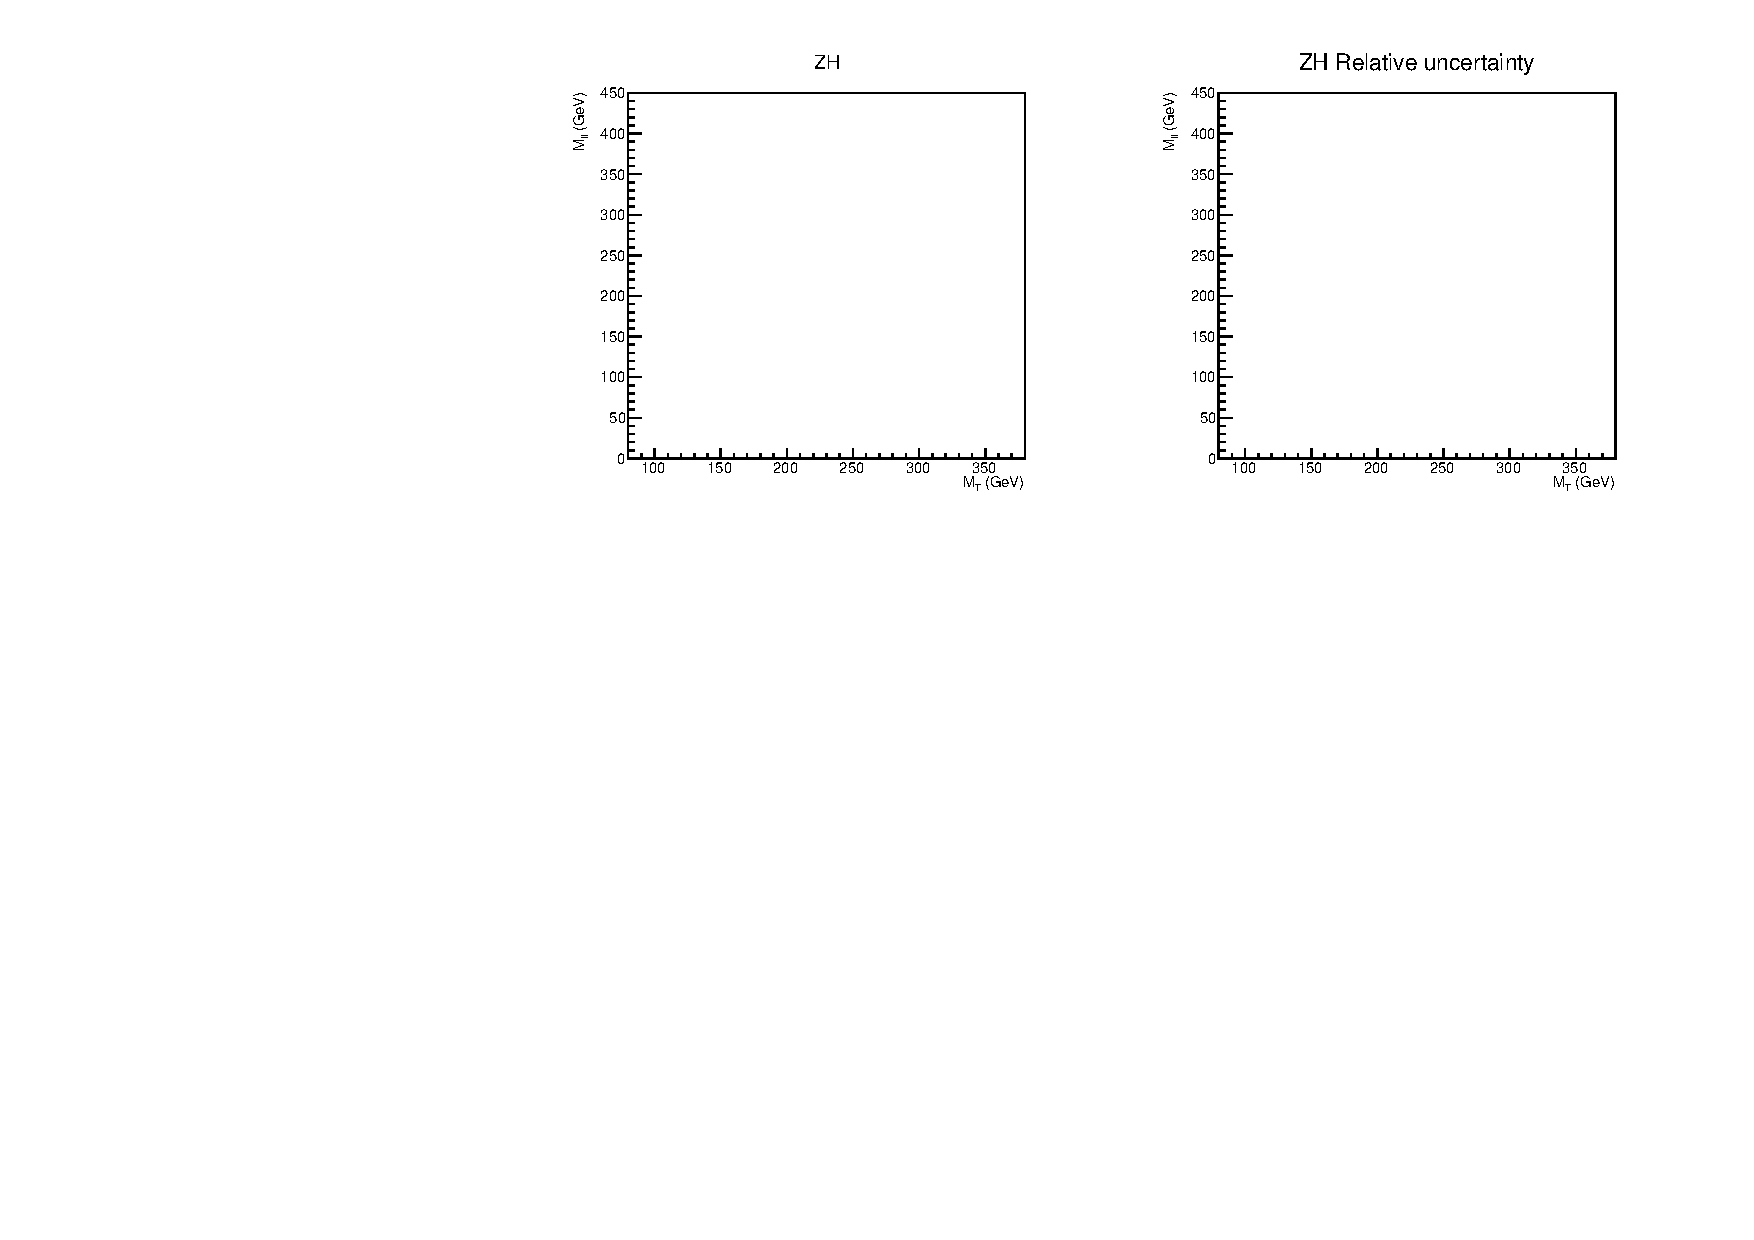
\includegraphics[width=0.8\textwidth]{figures/2dtemplate_ZH_mH400_0j.pdf}
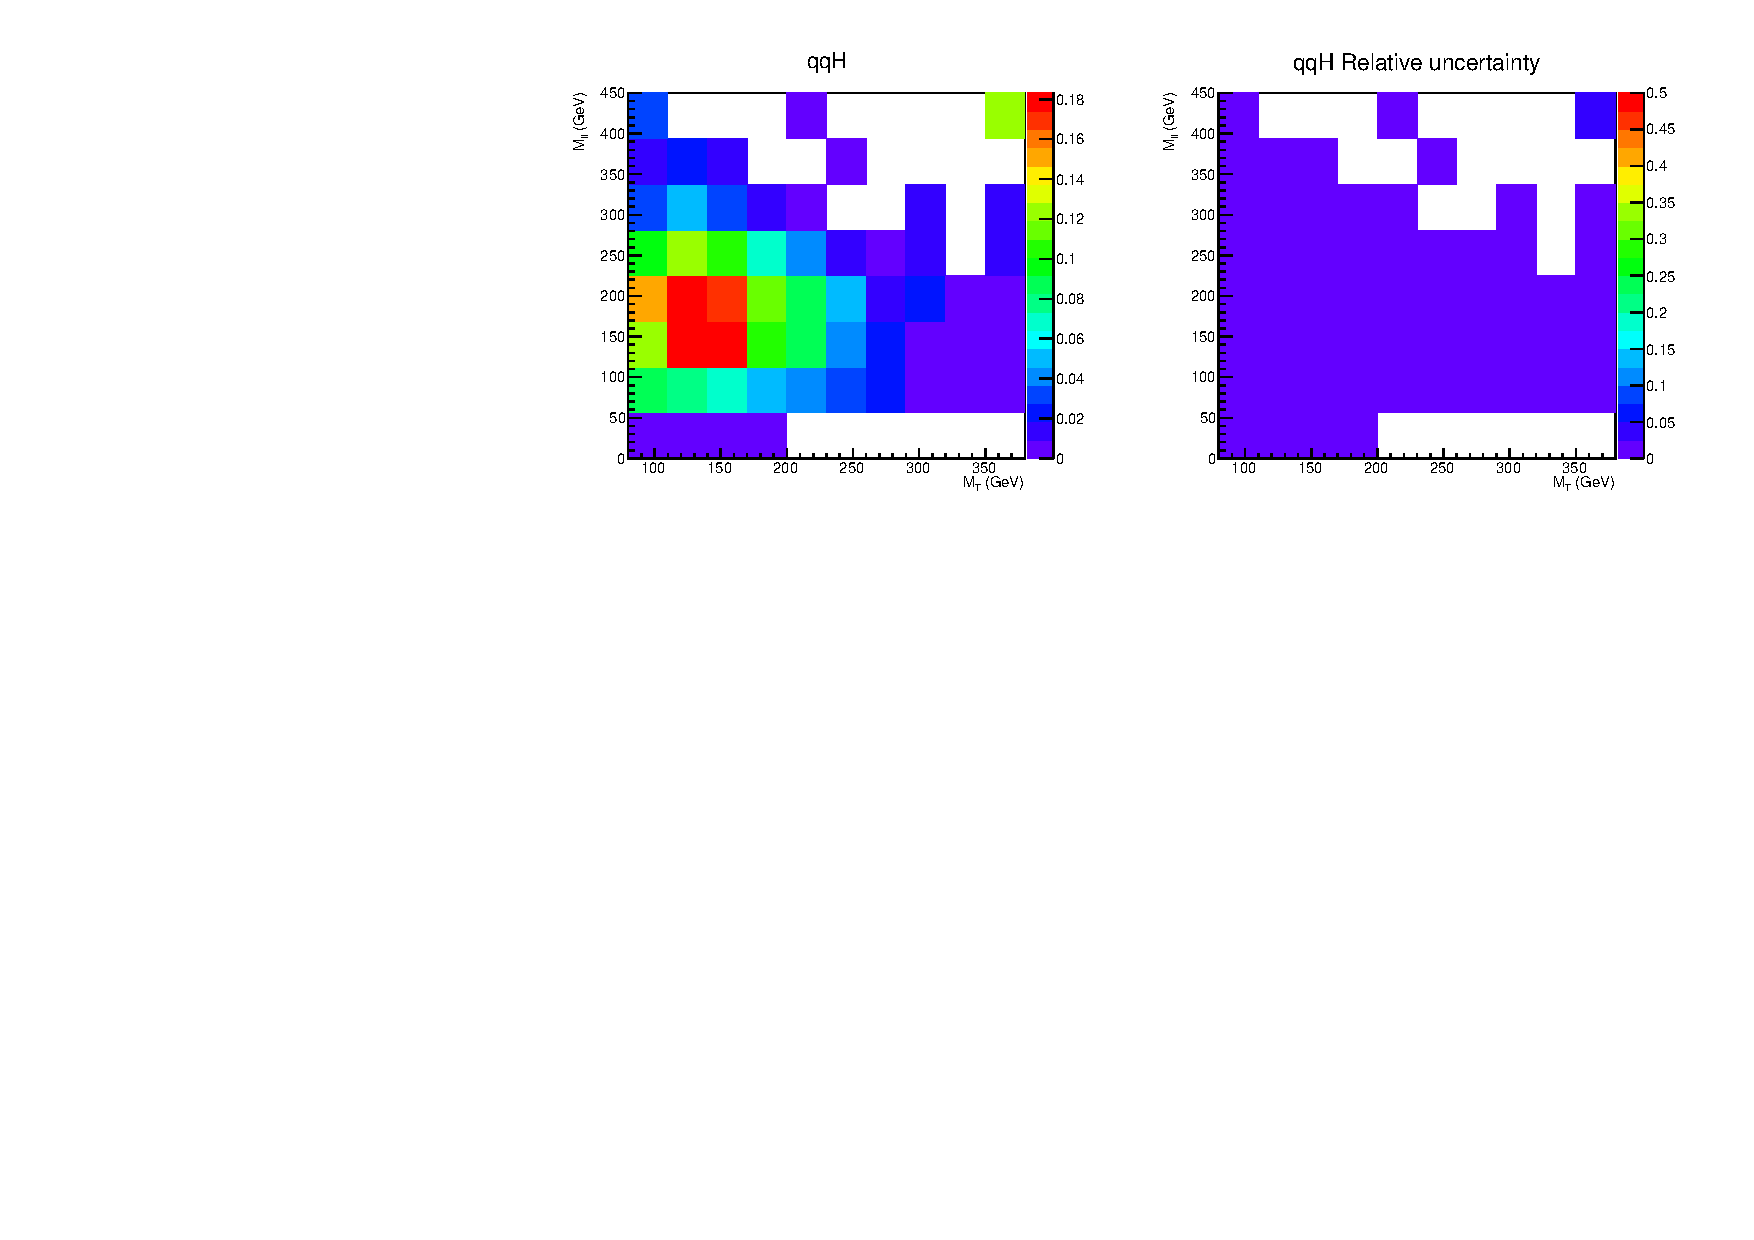
\includegraphics[width=0.8\textwidth]{figures/2dtemplate_qqH_mH400_0j.pdf}
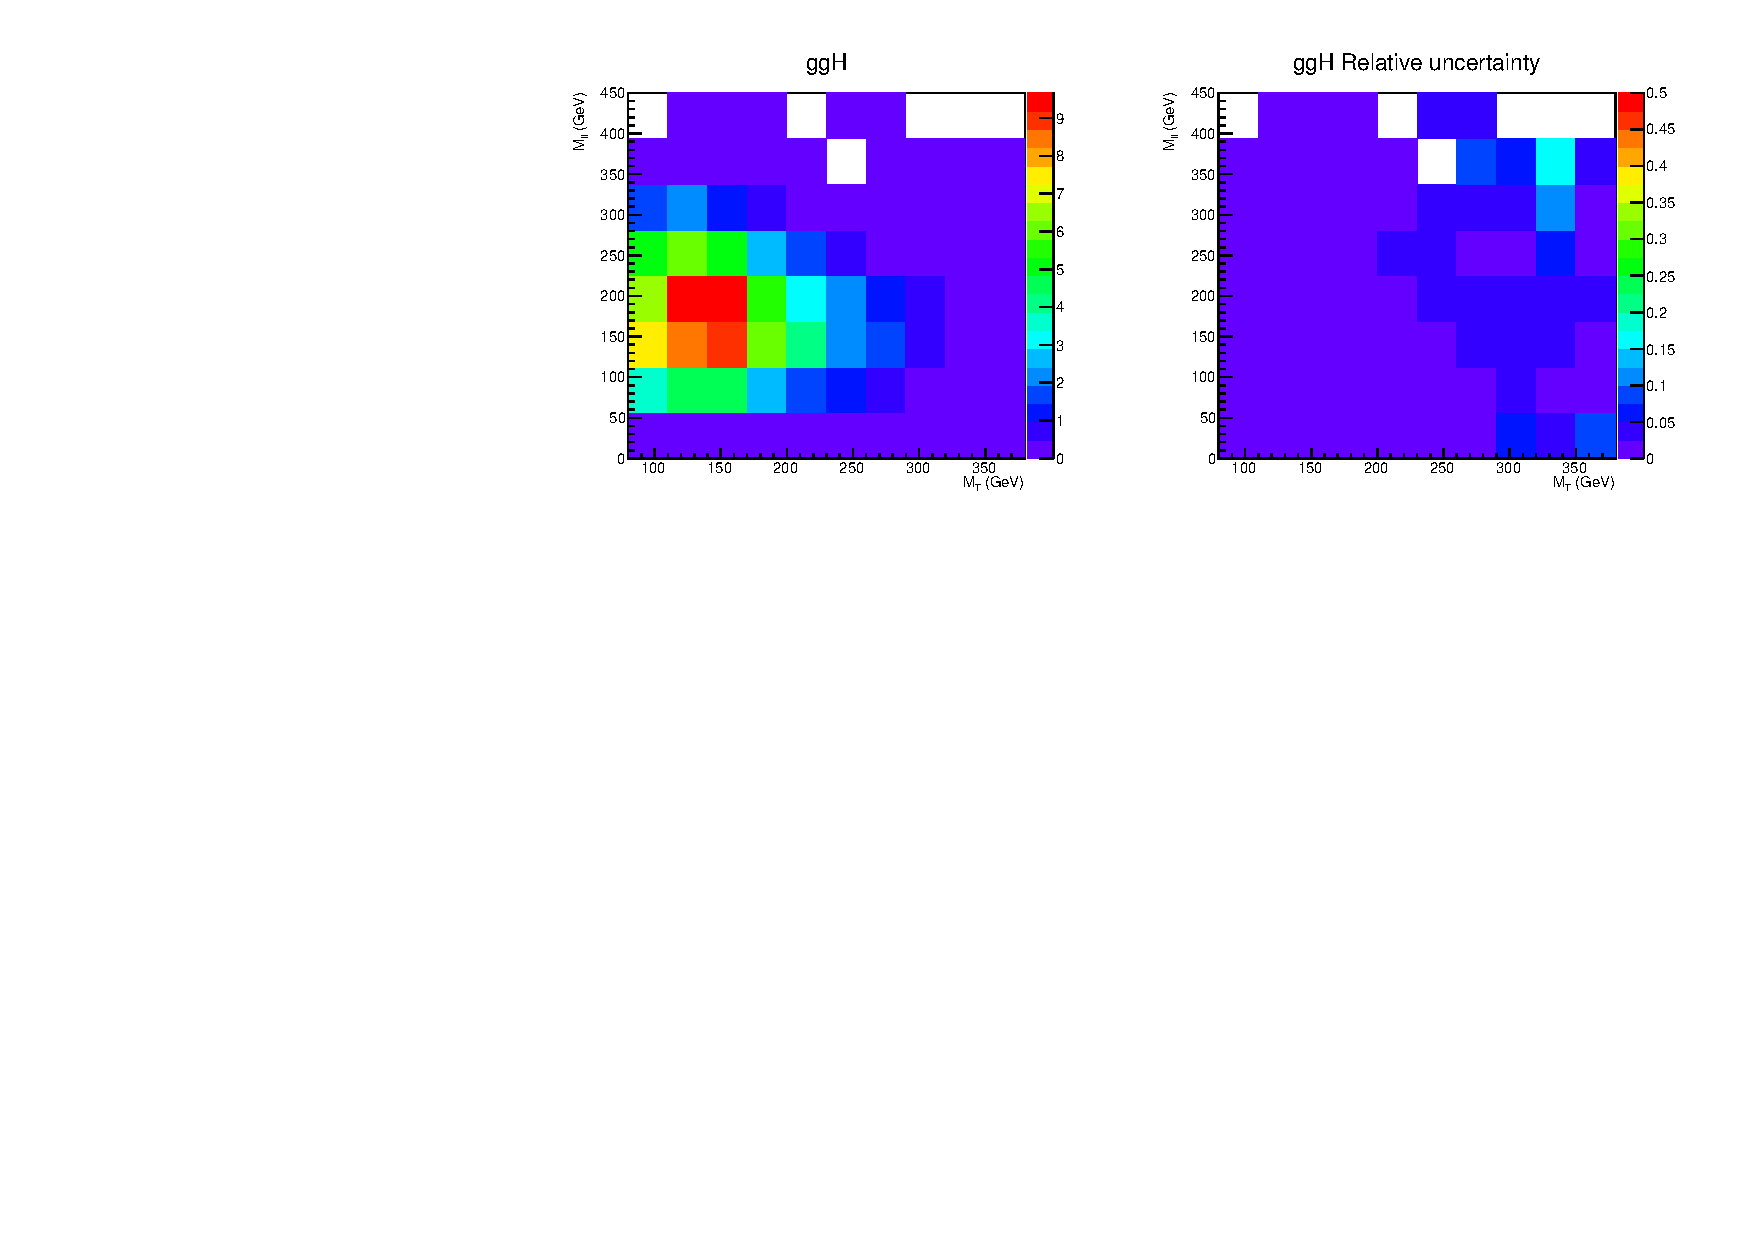
\includegraphics[width=0.8\textwidth]{figures/2dtemplate_ggH_mH400_0j.pdf}
\caption{Templates(left) and relative statistical uncertainty of the MC sample(right) 
of \qqWH, \qqZH, \qqH\ and \ggH. 
The templates are for \mHi\ = 400 \GeV\ analysis in the 0-jet category.}
\label{fig:2dtemplate_400_0j_1}
\end{figure}

\begin{figure}[htp]
\centering
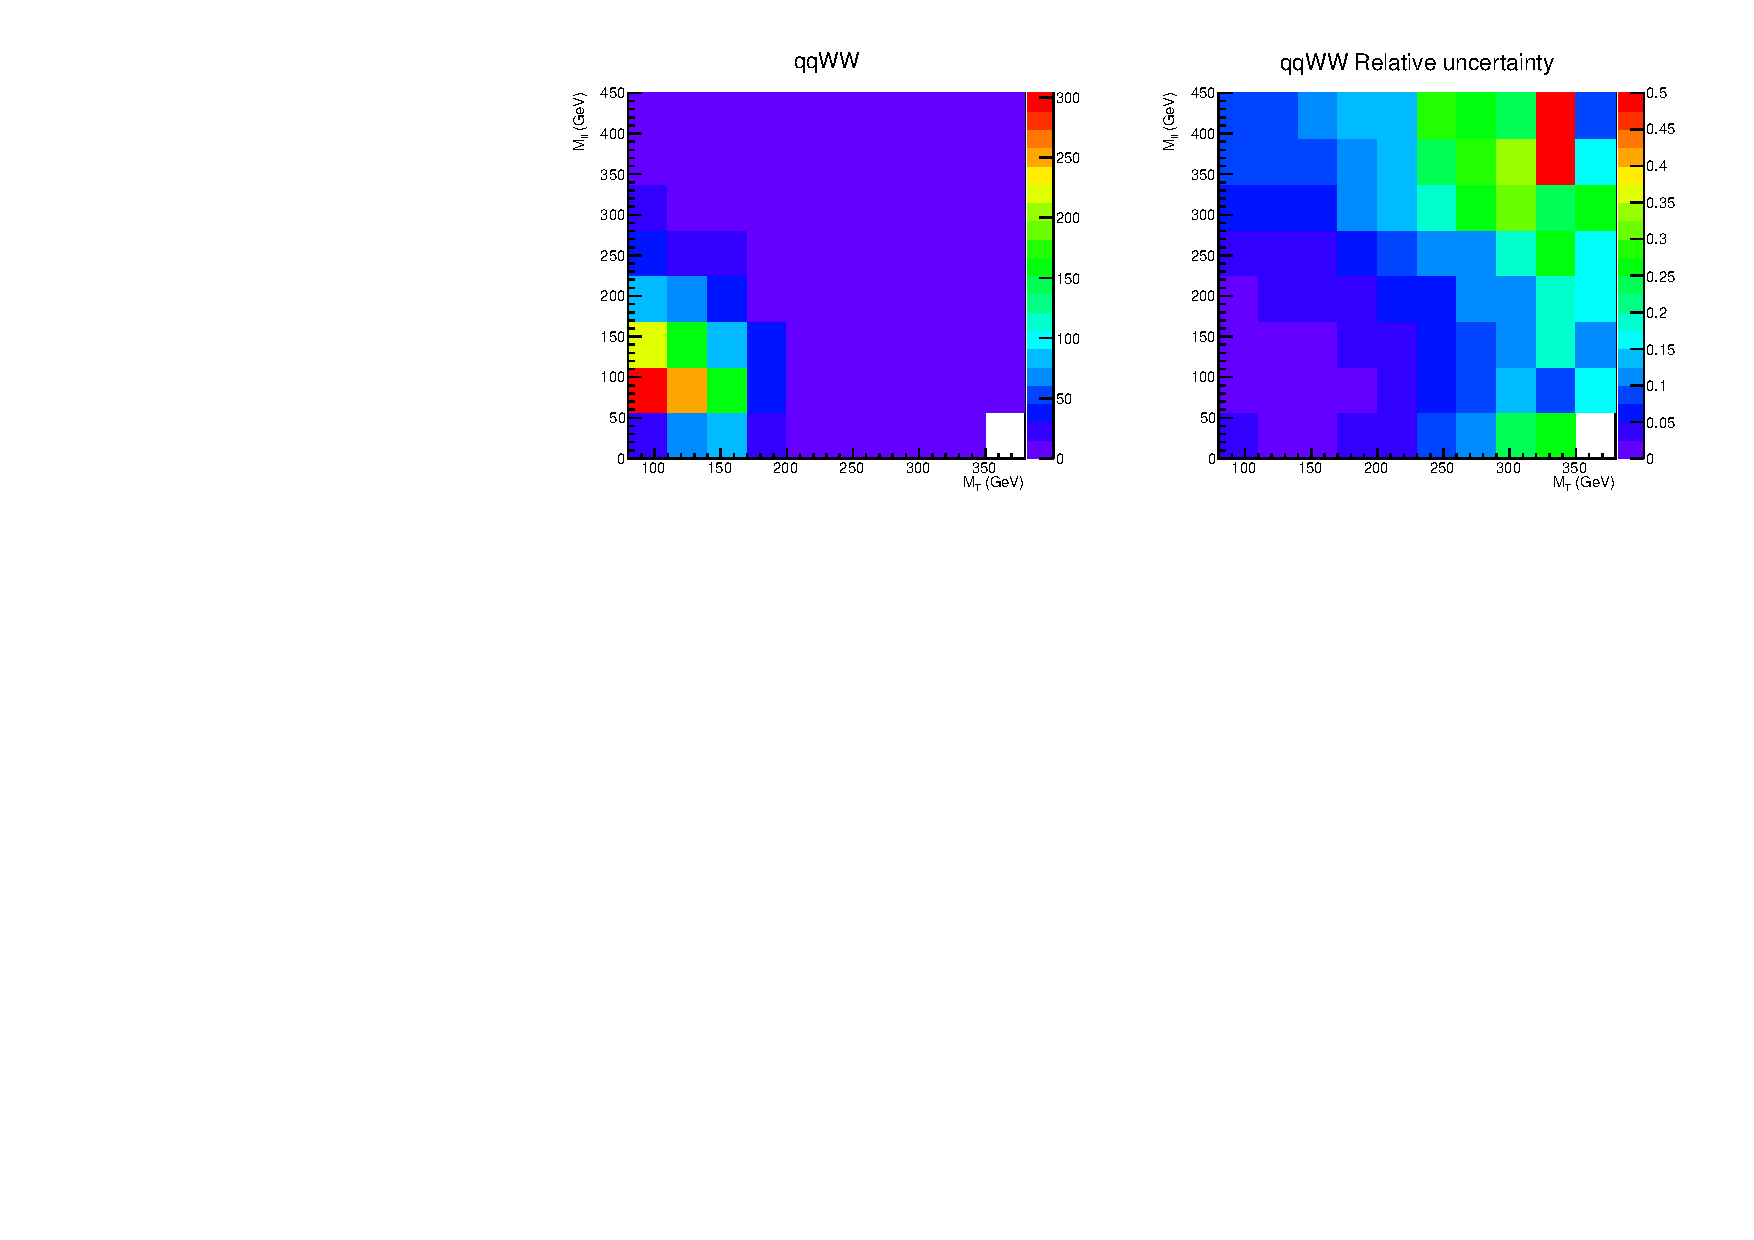
\includegraphics[width=0.8\textwidth]{figures/2dtemplate_qqWW_mH400_0j.pdf}
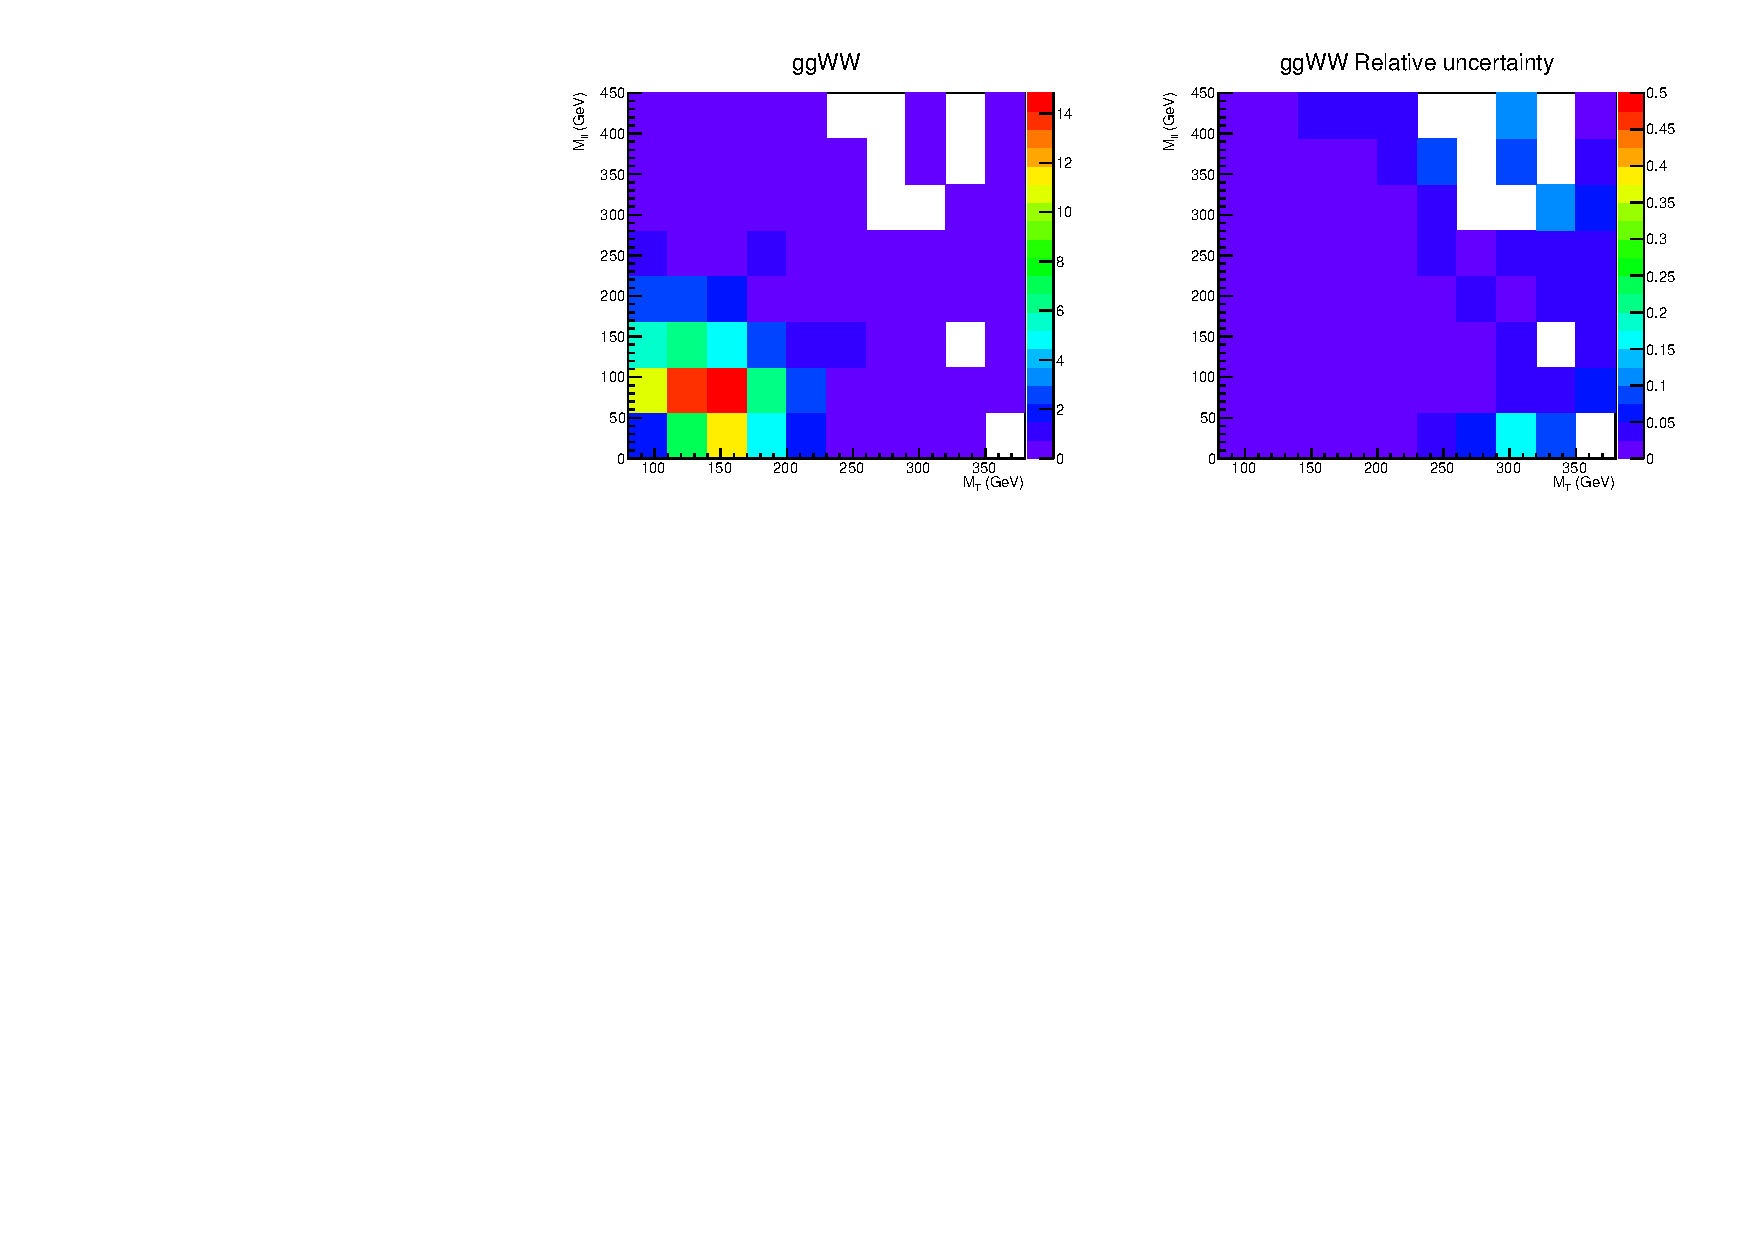
\includegraphics[width=0.8\textwidth]{figures/2dtemplate_ggWW_mH400_0j.pdf}
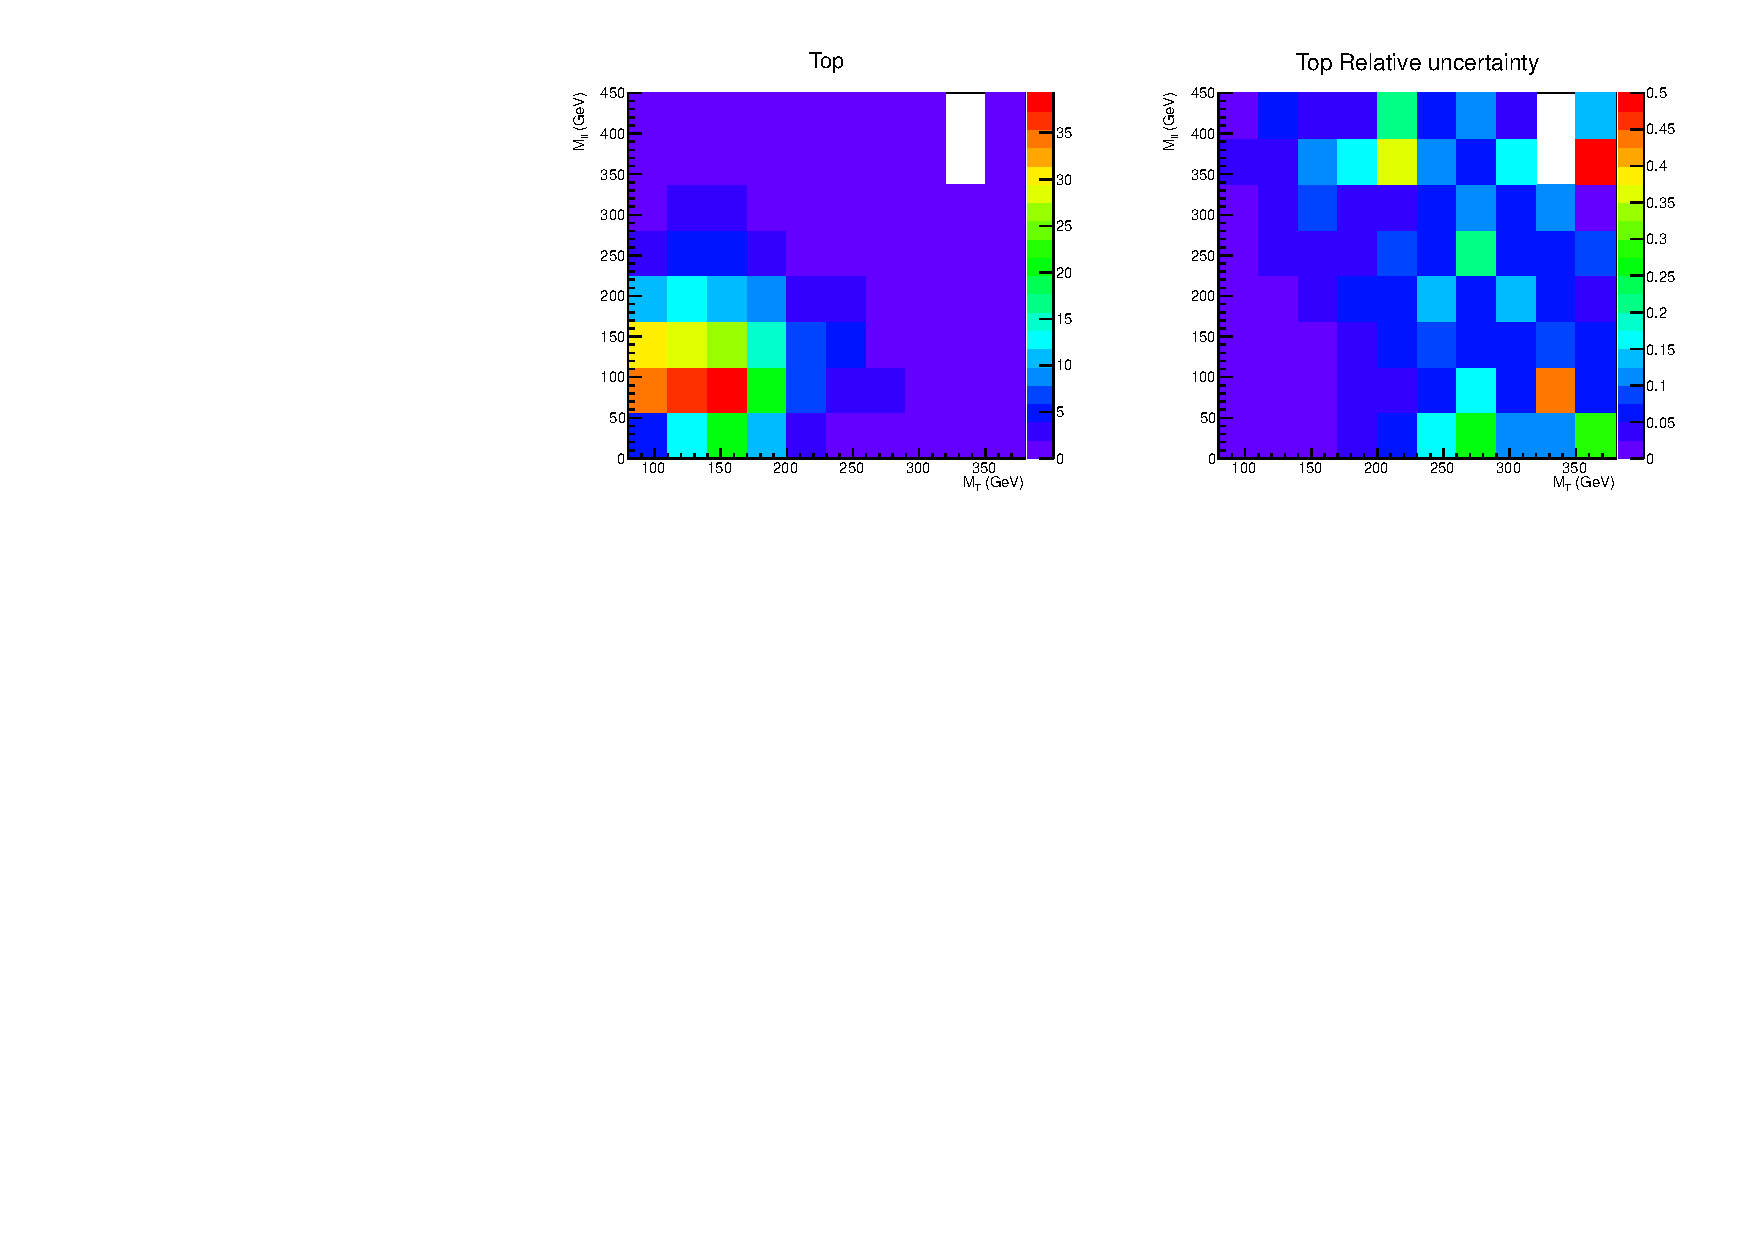
\includegraphics[width=0.8\textwidth]{figures/2dtemplate_Top_mH400_0j.pdf}
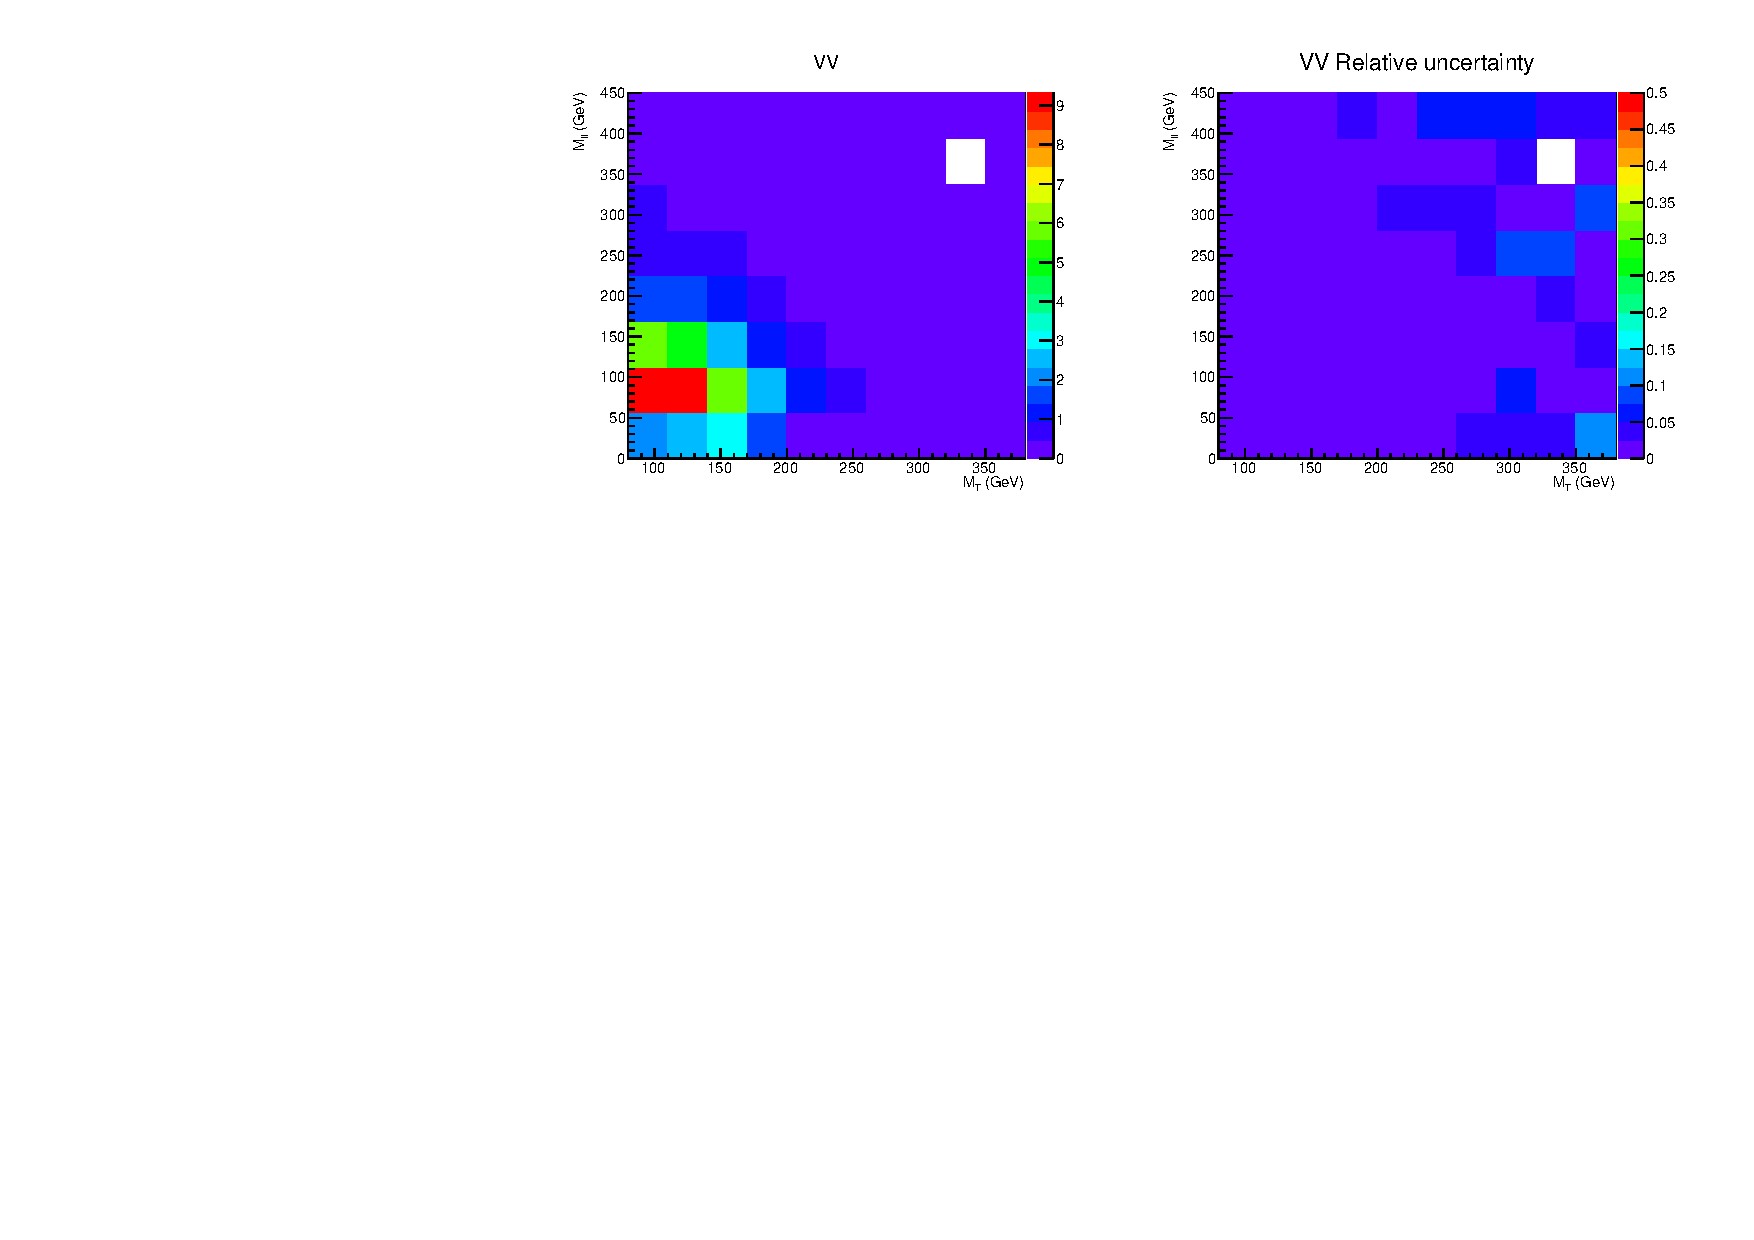
\includegraphics[width=0.8\textwidth]{figures/2dtemplate_VV_mH400_0j.pdf}
\caption{Templates(left) and relative statistical uncertainty of the MC sample(right) 
of \qqww, \ggww, \topbkg\ and \vv. 
The templates are for \mHi\ = 400 \GeV\ analysis in the 0-jet category.}
\label{fig:2dtemplate_400_0j_2}
\end{figure}

\begin{figure}[htp]
\centering
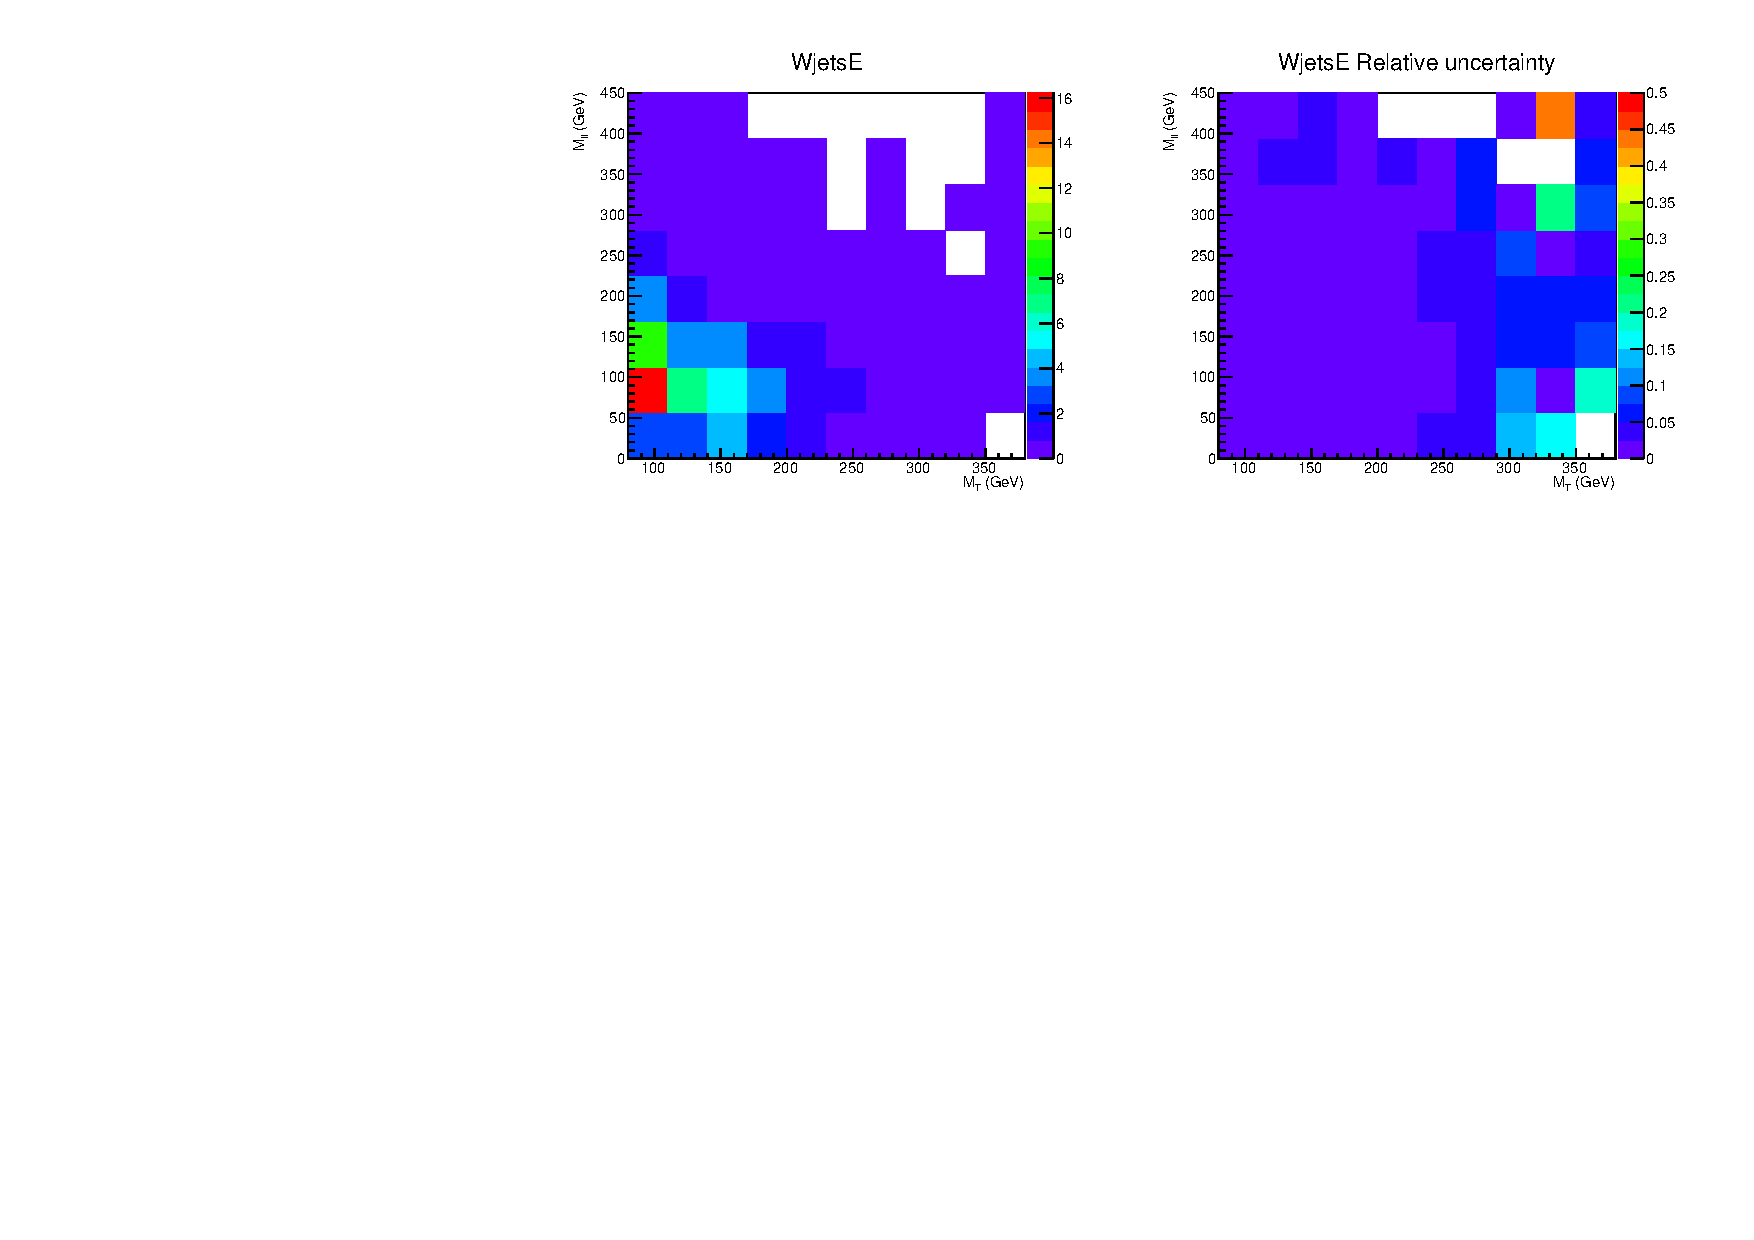
\includegraphics[width=0.8\textwidth]{figures/2dtemplate_WjetsE_mH400_0j.pdf}
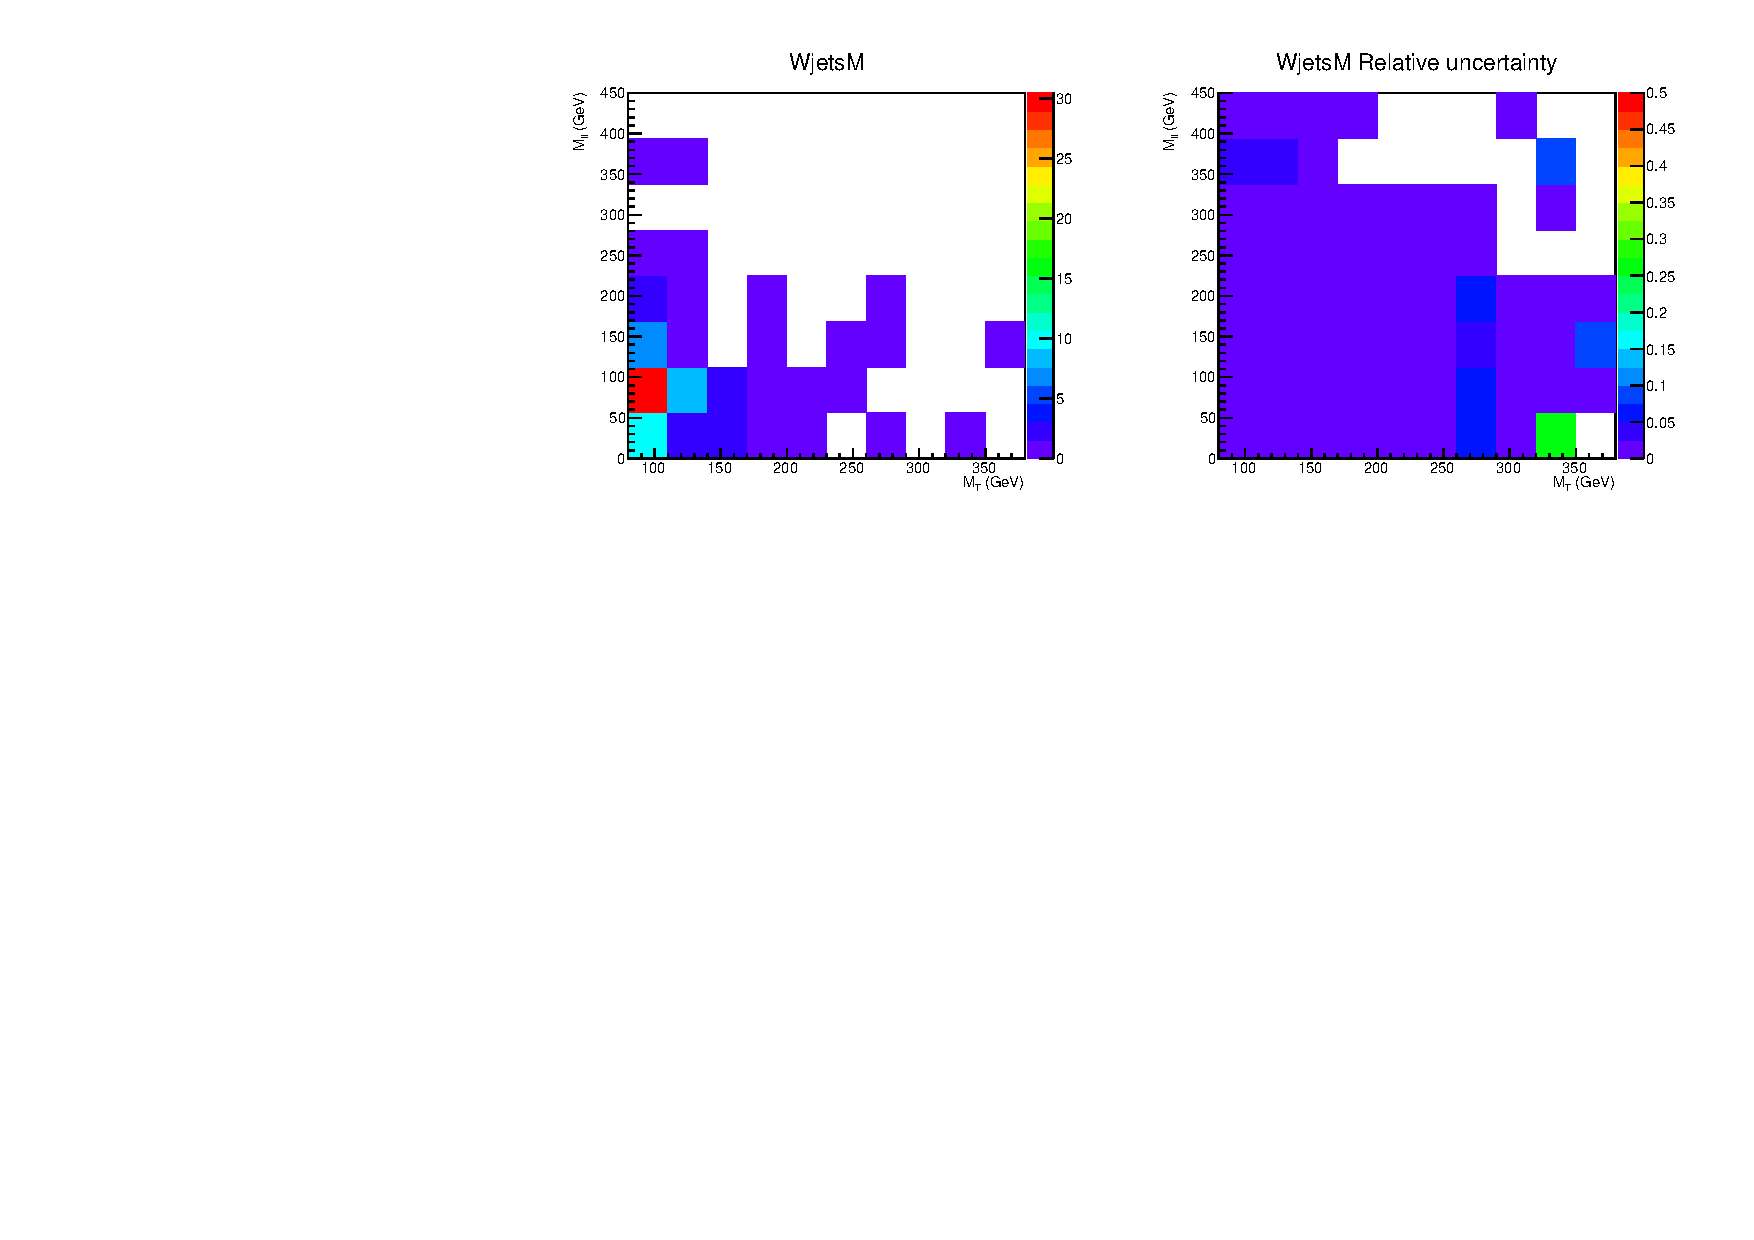
\includegraphics[width=0.8\textwidth]{figures/2dtemplate_WjetsM_mH400_0j.pdf}
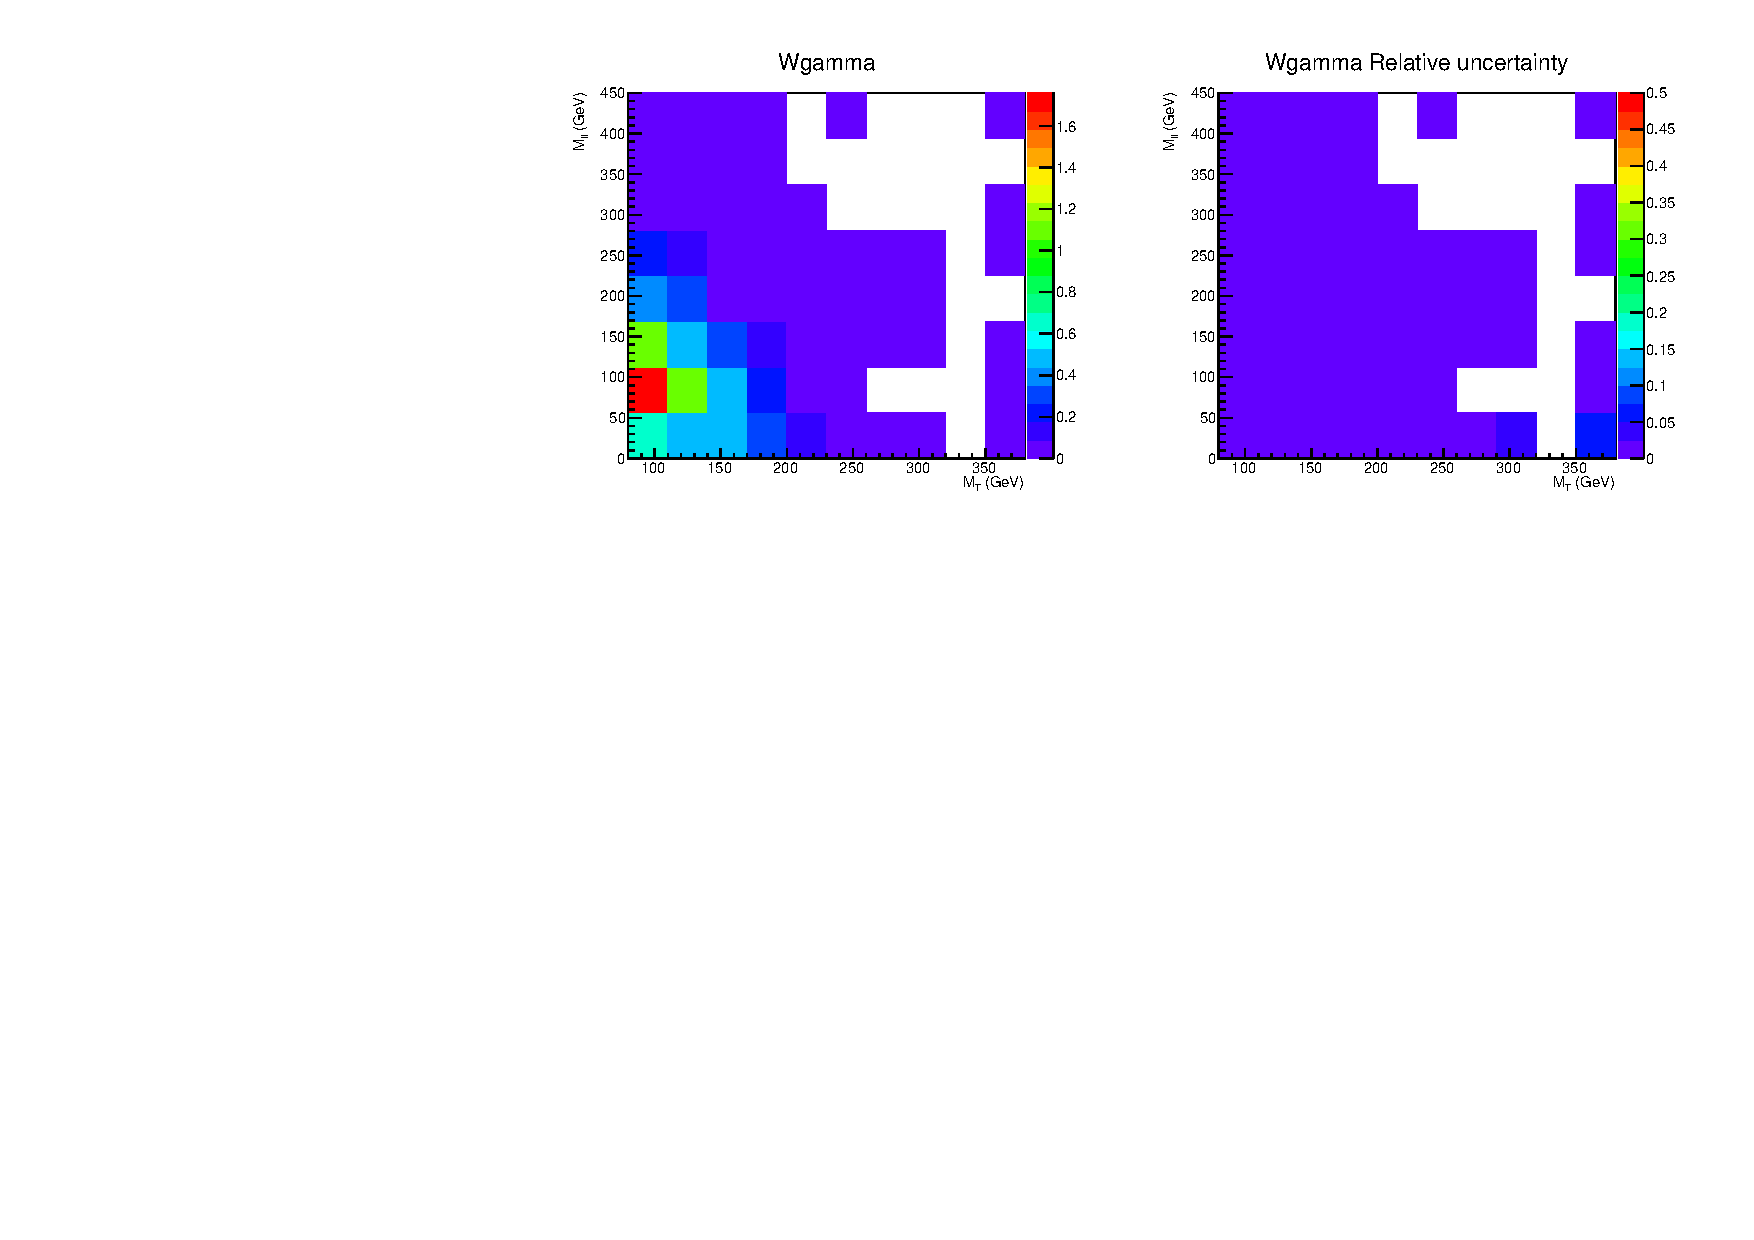
\includegraphics[width=0.8\textwidth]{figures/2dtemplate_Wgamma_mH400_0j.pdf}
\caption{Templates(left) and relative statistical uncertainty of the MC sample(right) 
of \WjetsE, \WjetsM\ and \wgamma. 
The templates are for \mHi\ = 400 \GeV\ analysis in the 0-jet category.}
\label{fig:2dtemplate_400_0j_3}
\end{figure}

\begin{figure}[htp]
\centering
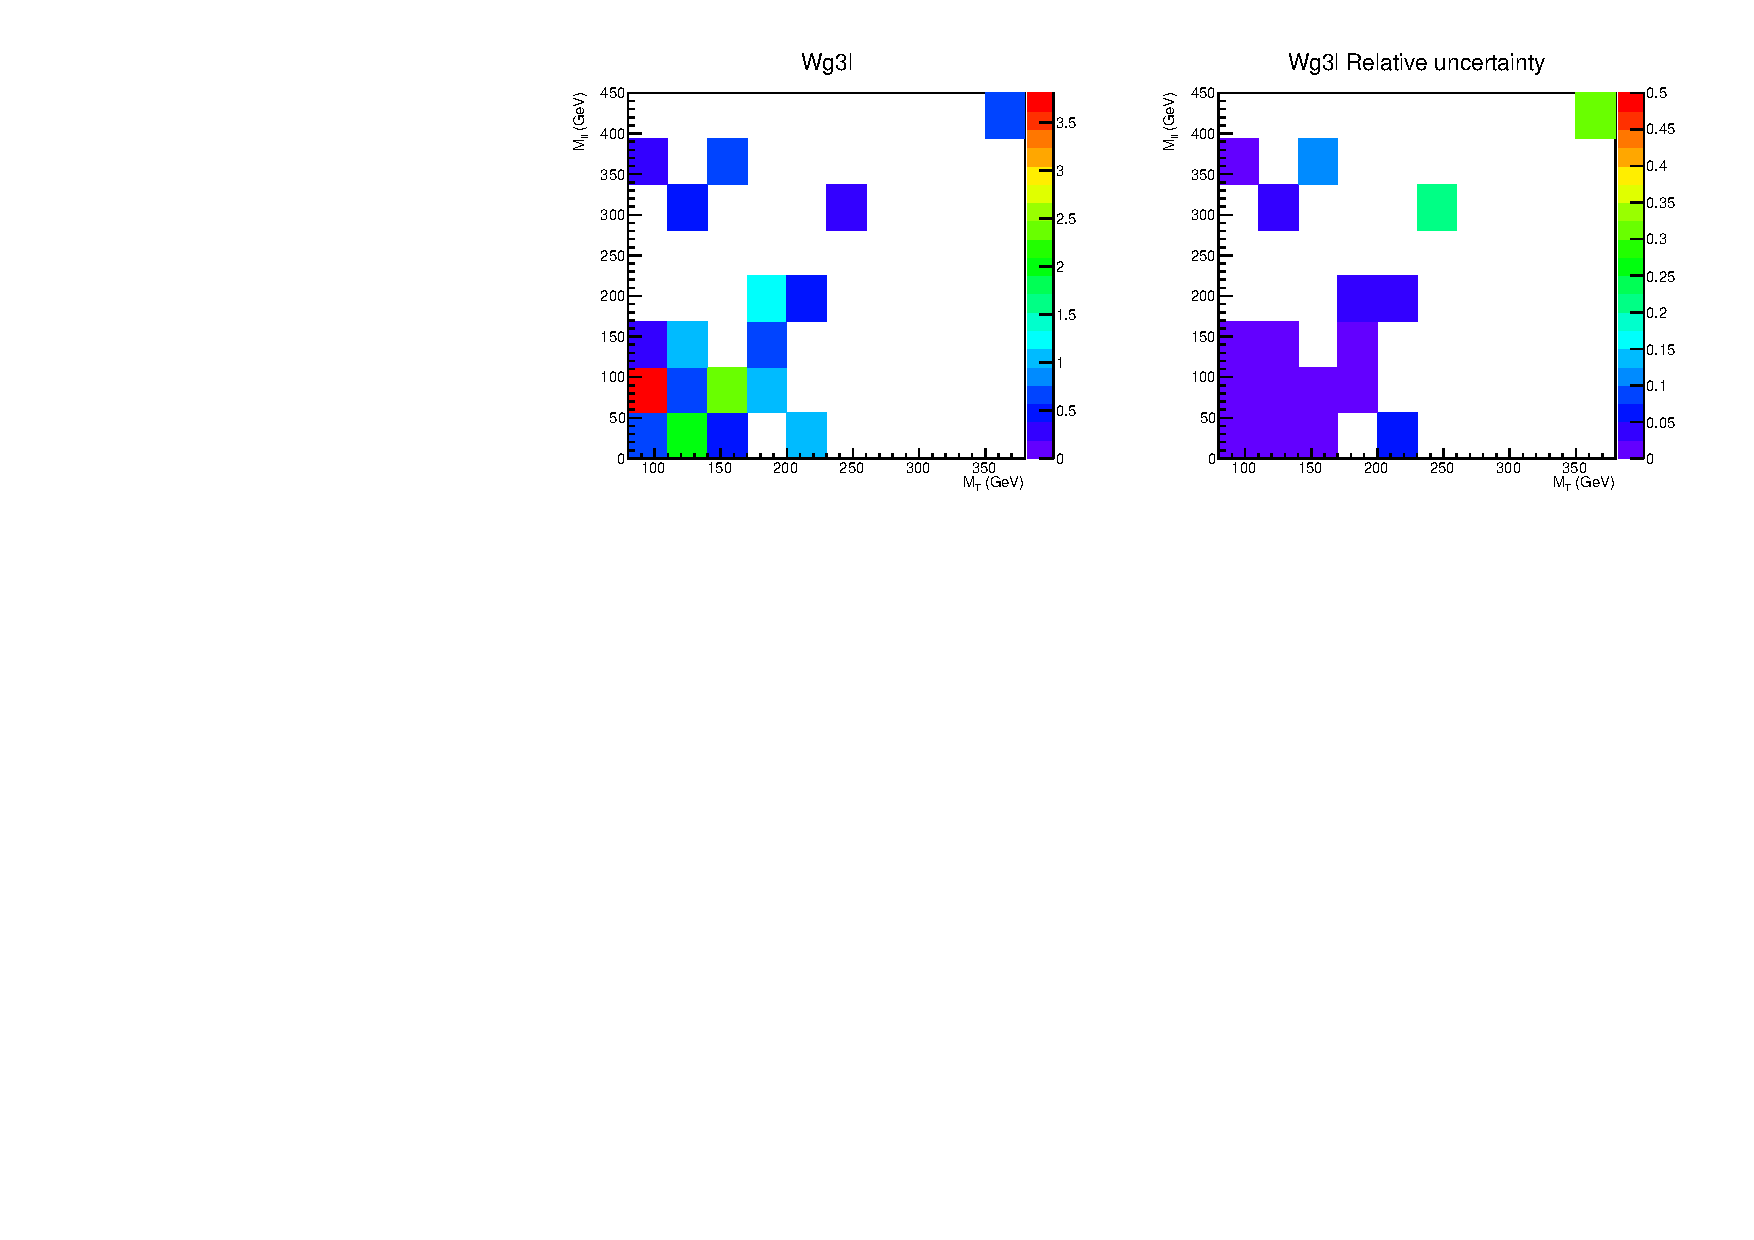
\includegraphics[width=0.8\textwidth]{figures/2dtemplate_Wg3l_mH400_0j.pdf}
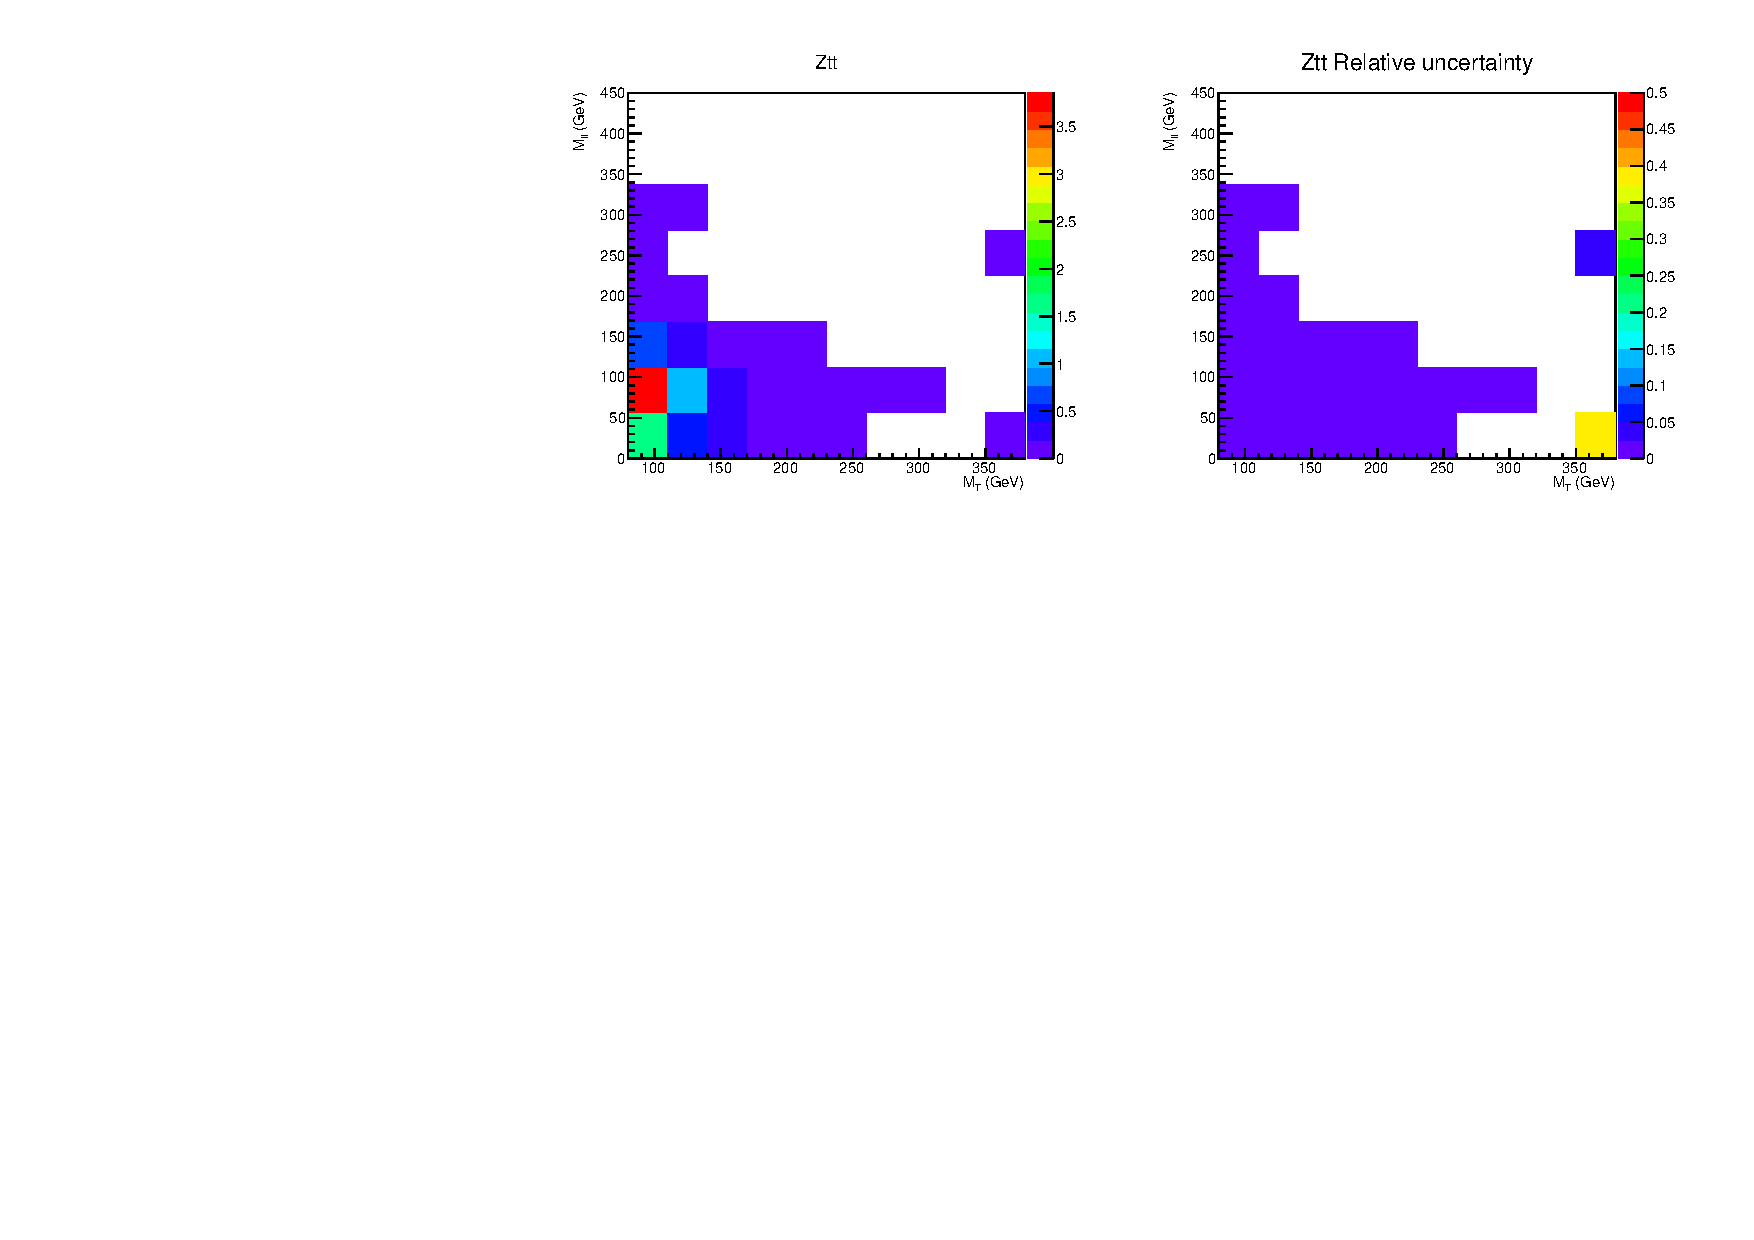
\includegraphics[width=0.8\textwidth]{figures/2dtemplate_Ztt_mH400_0j.pdf}
\caption{Templates(left) and relative statistical uncertainty of the MC sample(right) 
of \wgammastar\ and \ztt. 
The templates are for \mHi\ = 400 \GeV\ analysis in the 0-jet category.}
\label{fig:2dtemplate_400_0j_4}
\end{figure} 



% 
% mH=400 GeV, 1-jet
% 
\begin{figure}[htp]
\centering
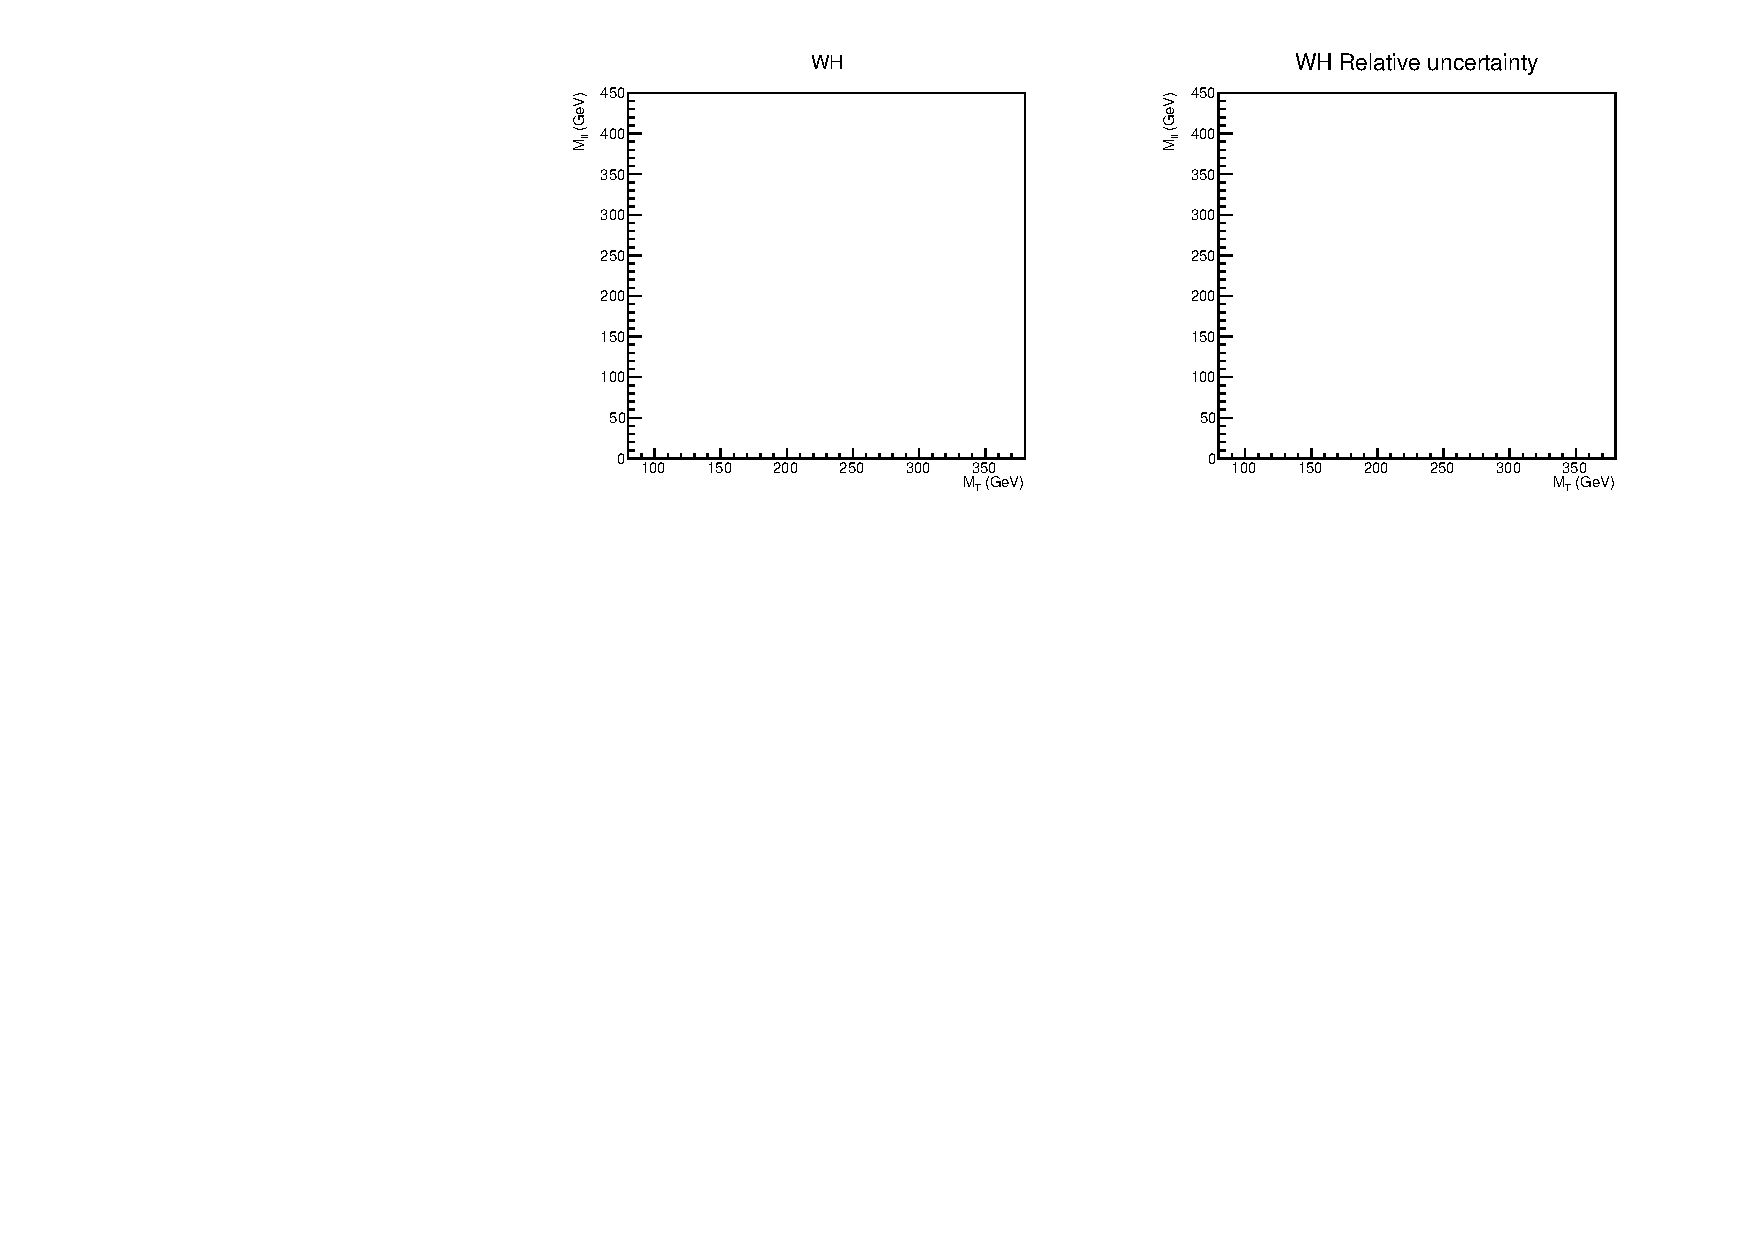
\includegraphics[width=0.8\textwidth]{figures/2dtemplate_WH_mH400_1j.pdf}
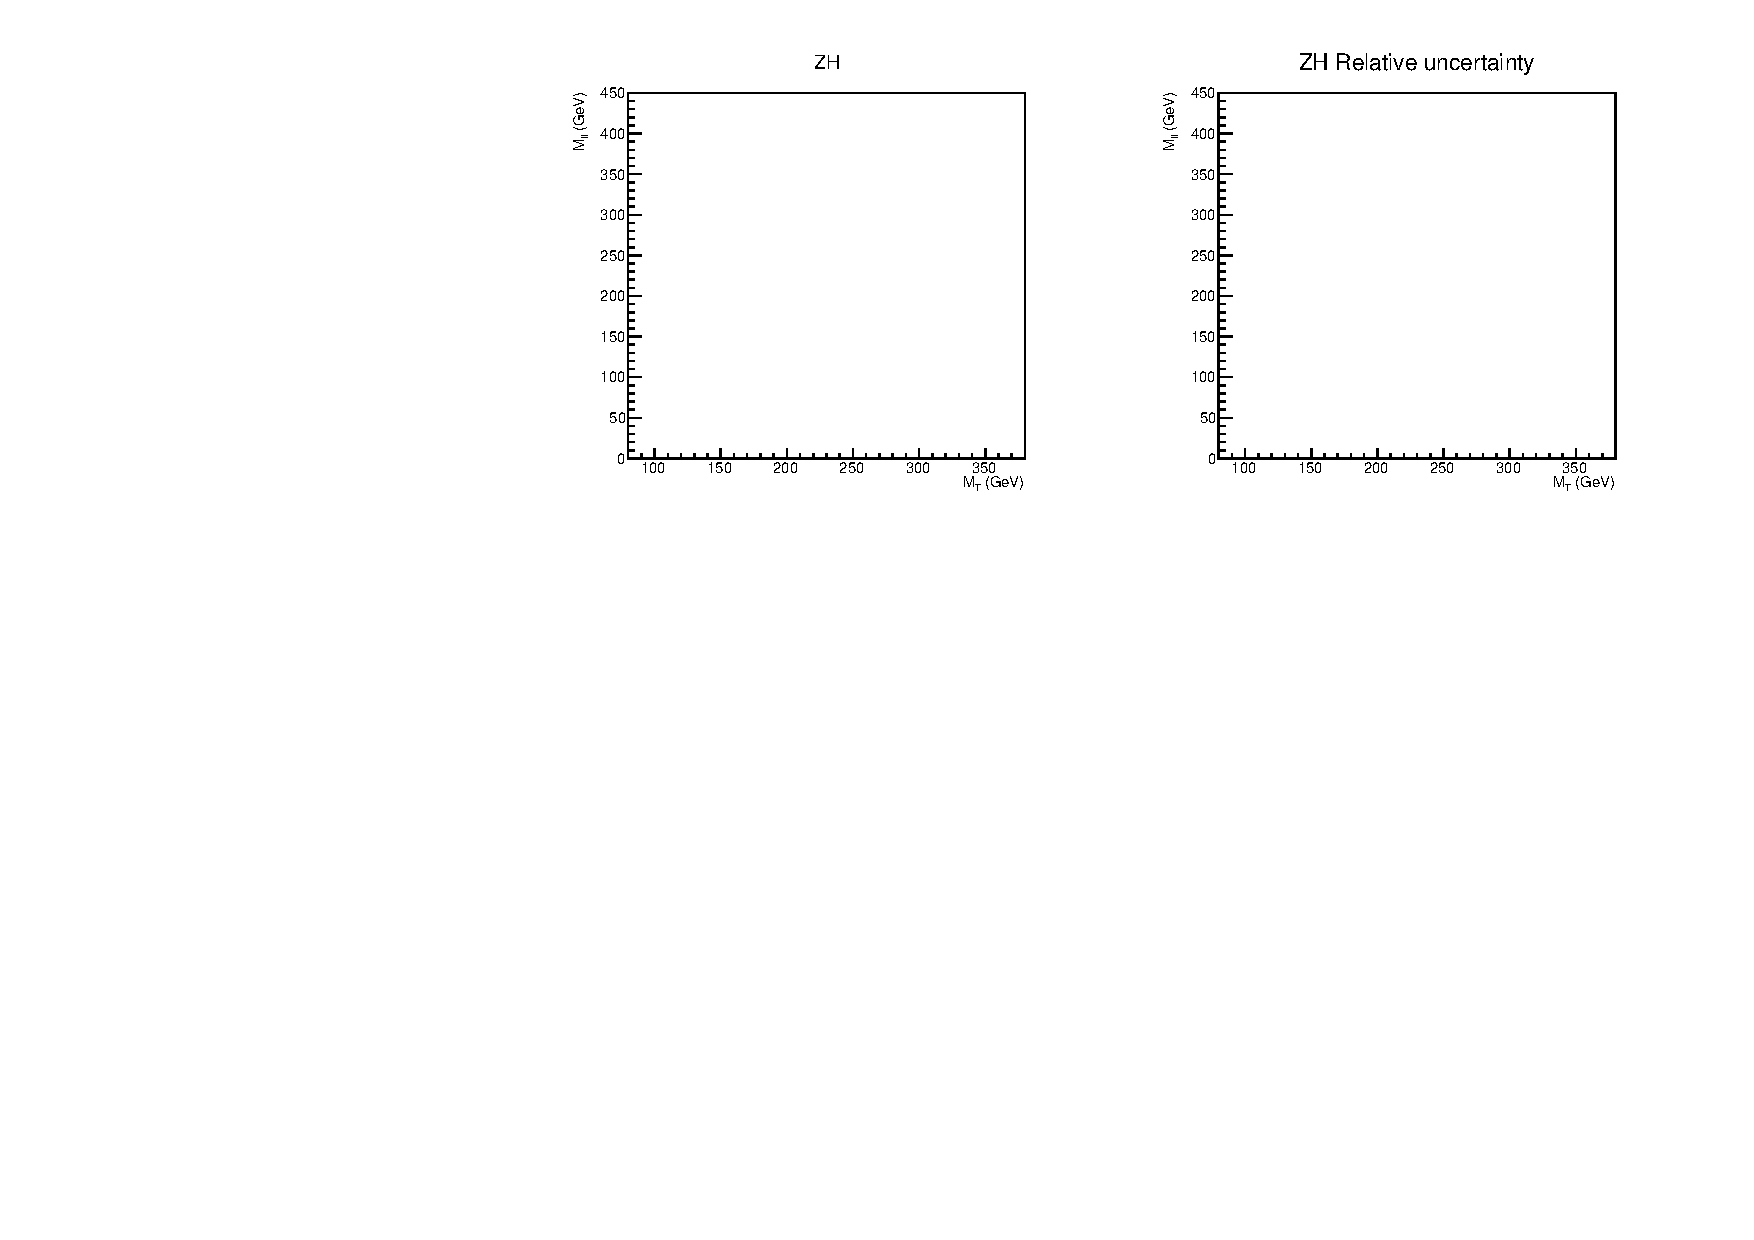
\includegraphics[width=0.8\textwidth]{figures/2dtemplate_ZH_mH400_1j.pdf}
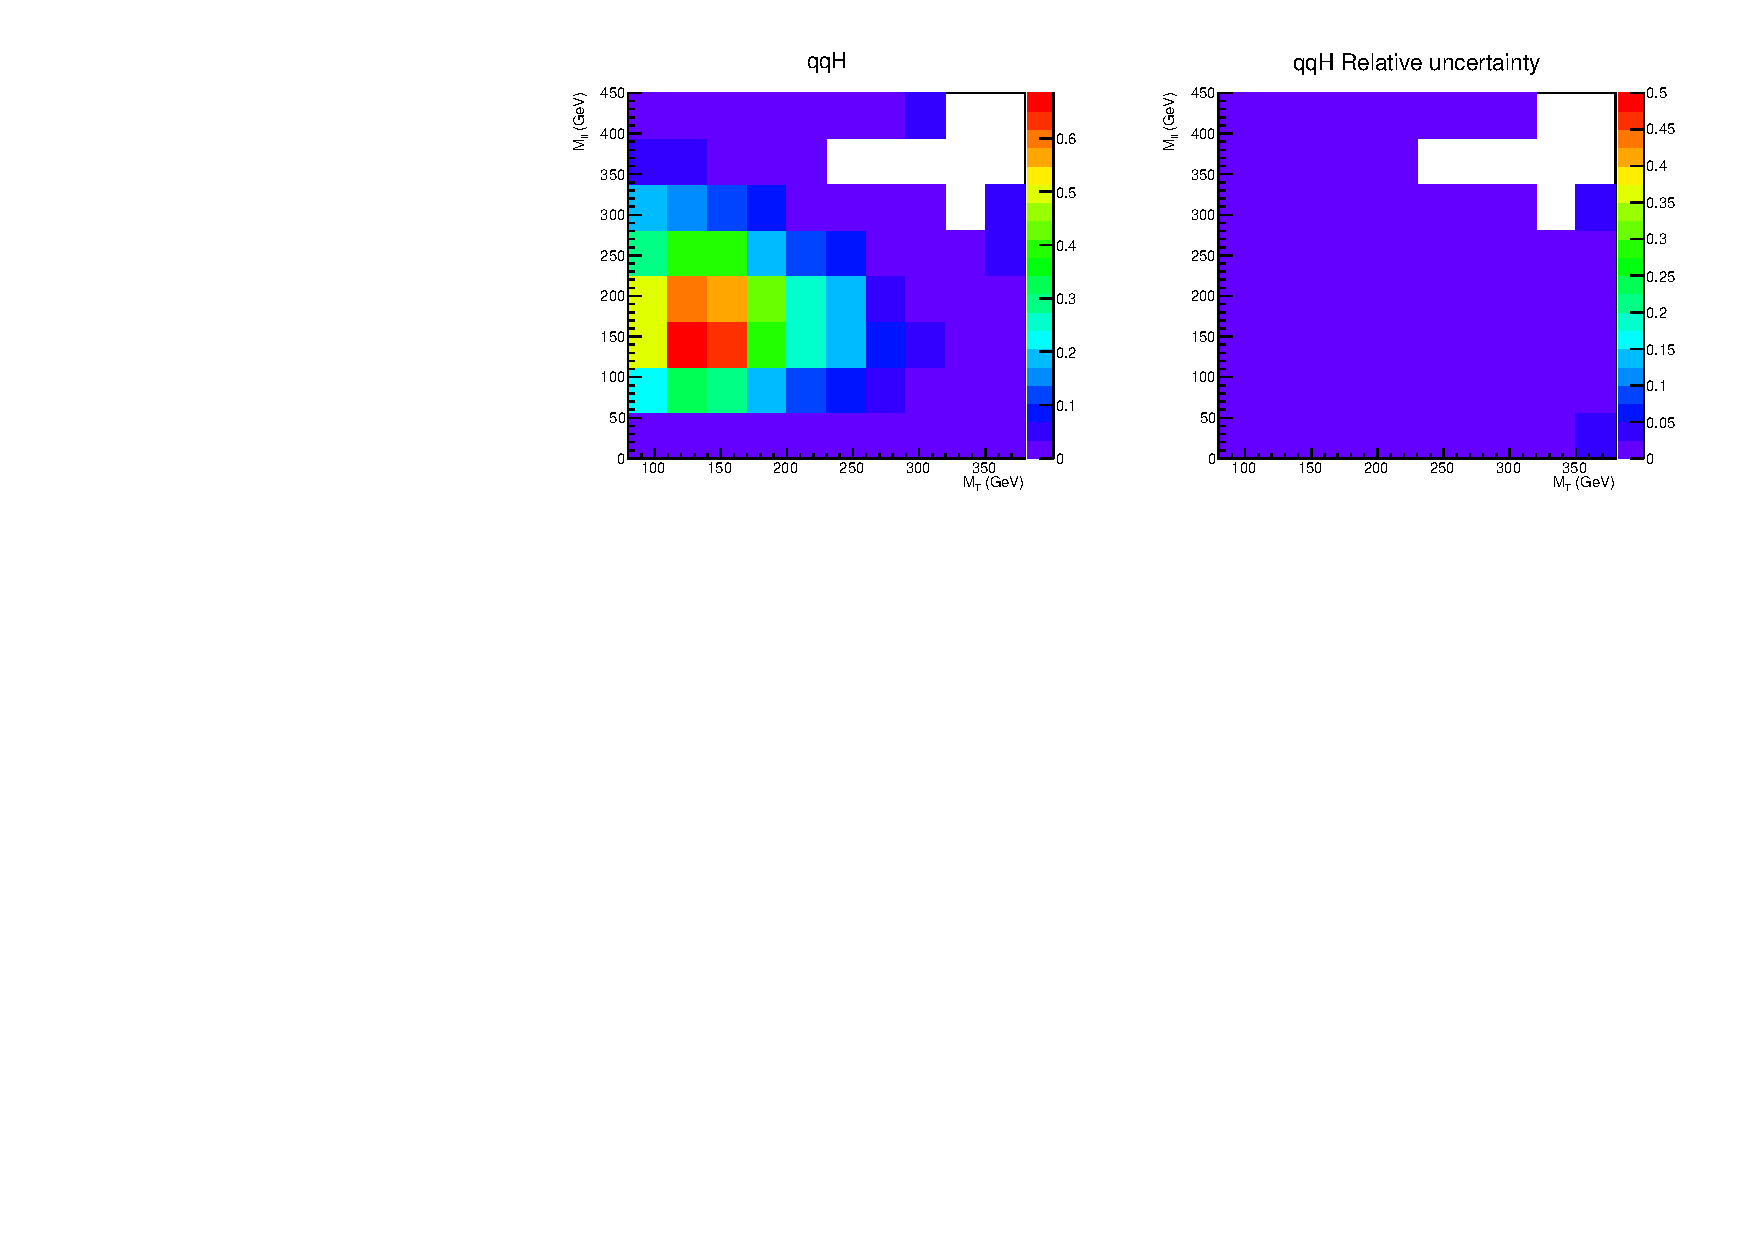
\includegraphics[width=0.8\textwidth]{figures/2dtemplate_qqH_mH400_1j.pdf}
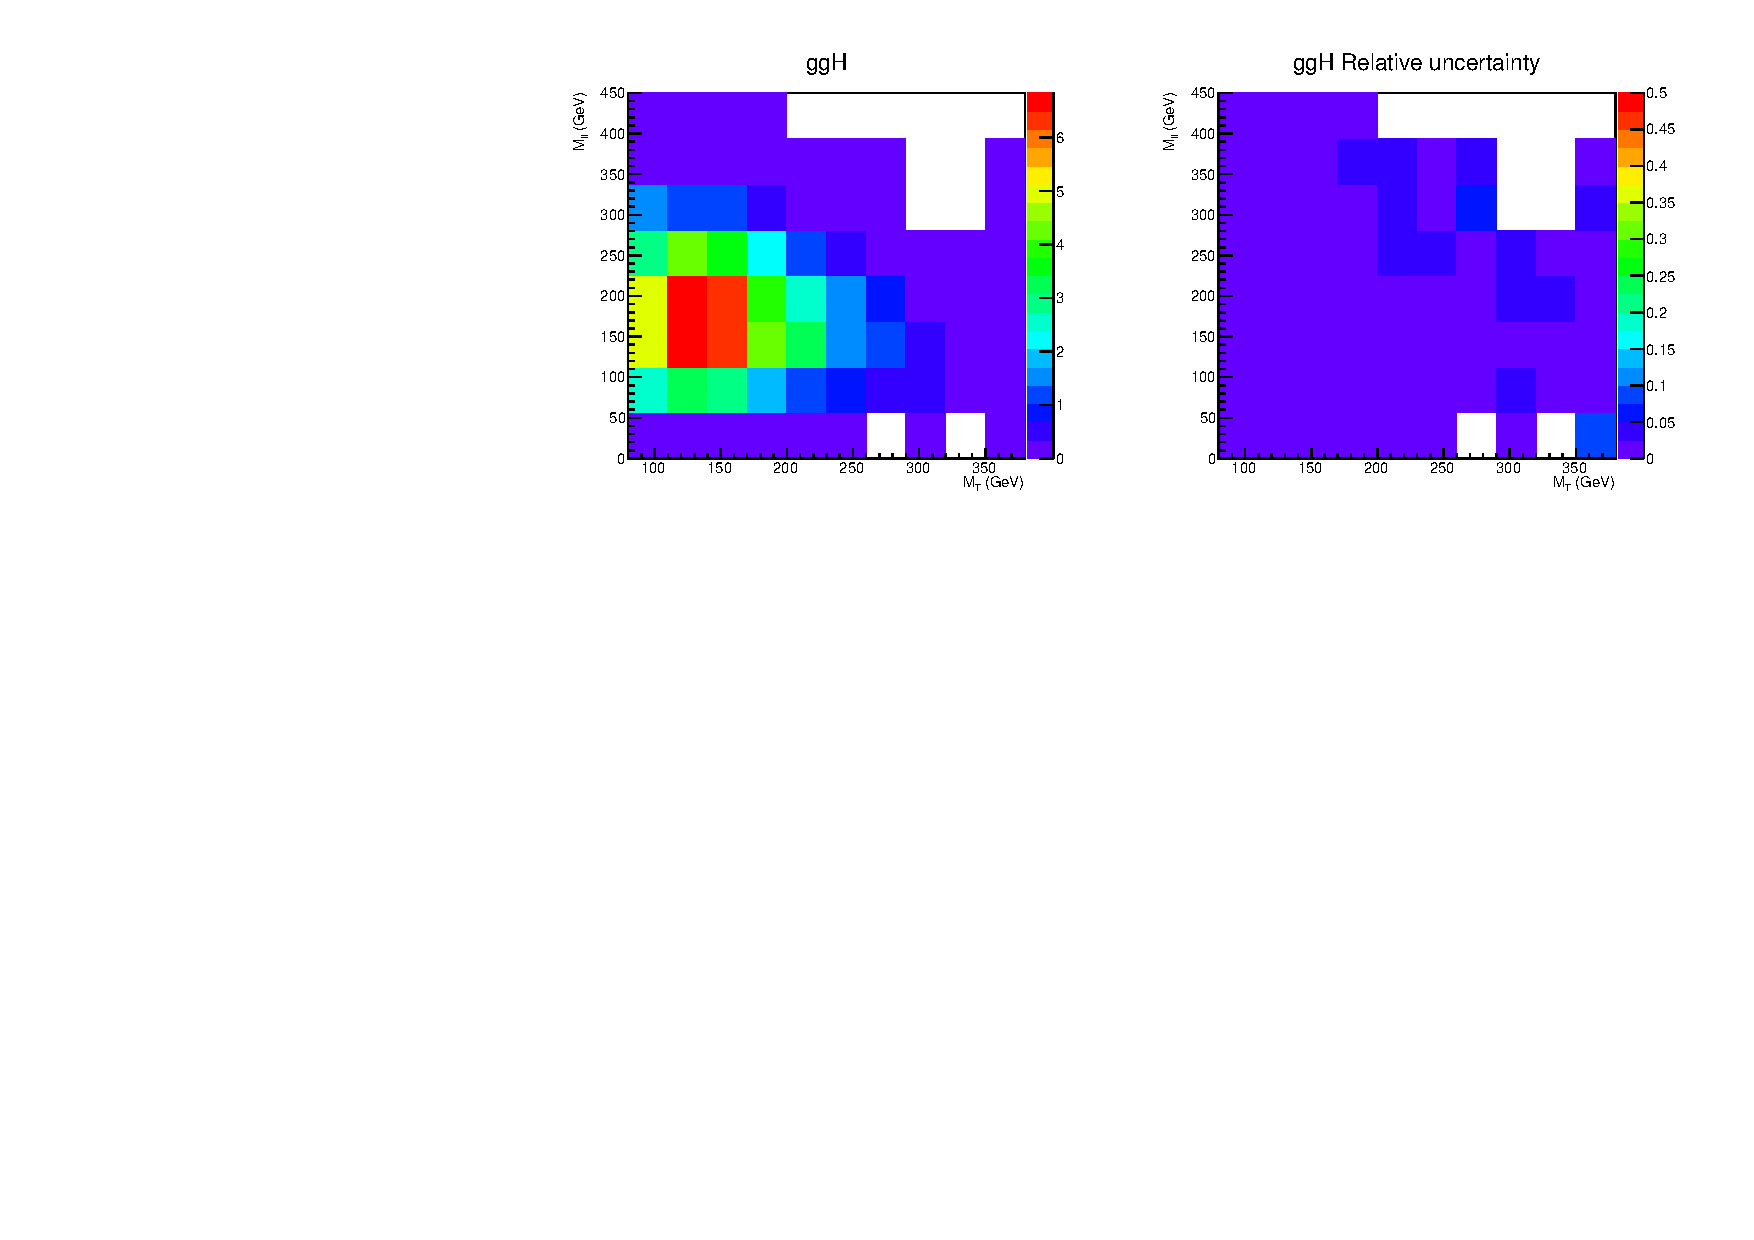
\includegraphics[width=0.8\textwidth]{figures/2dtemplate_ggH_mH400_1j.pdf}
\caption{Templates(left) and relative statistical uncertainty of the MC sample(right) 
of \qqWH, \qqZH, \qqH\ and \ggH. 
The templates are for \mHi\ = 400 \GeV\ analysis in the 1-jet category.}
\label{fig:2dtemplate_400_1j_1}
\end{figure}

\begin{figure}[htp]
\centering
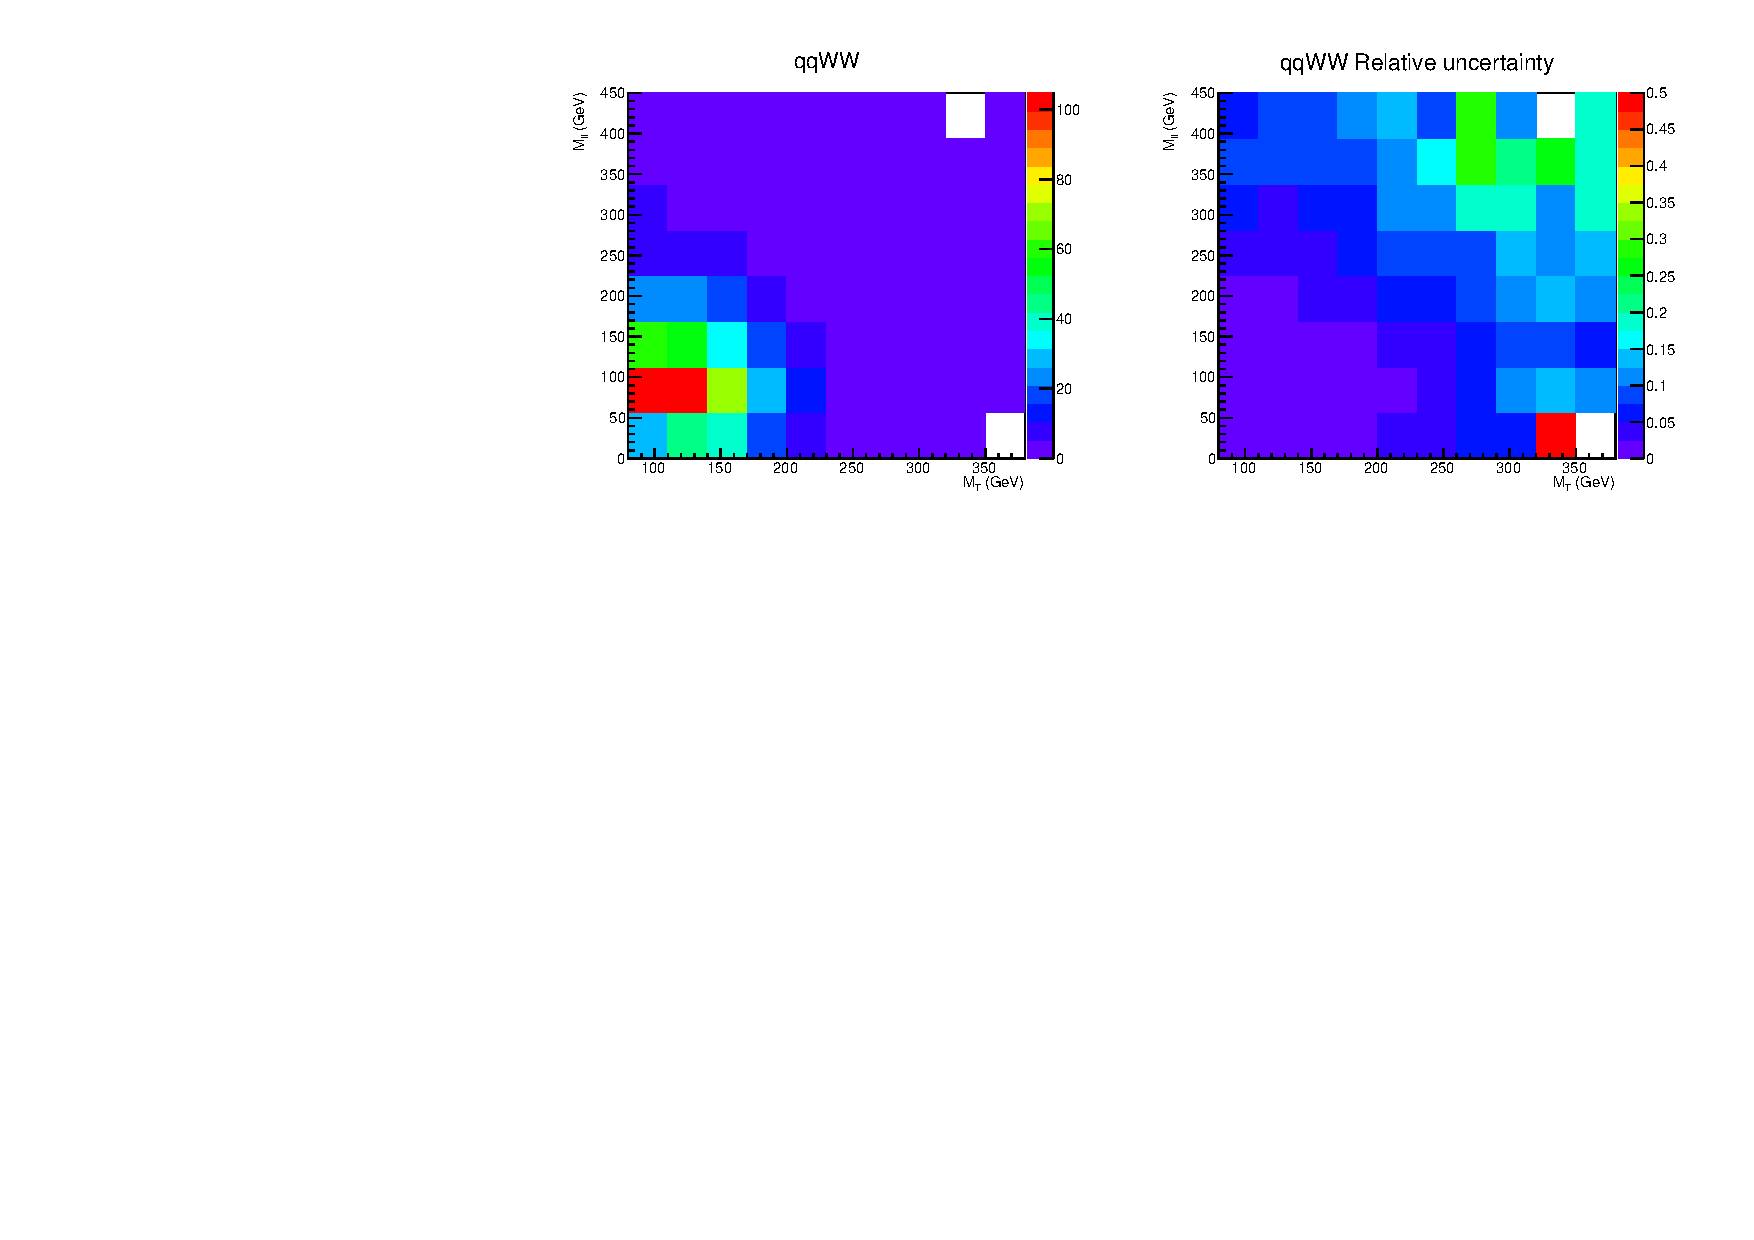
\includegraphics[width=0.8\textwidth]{figures/2dtemplate_qqWW_mH400_1j.pdf}
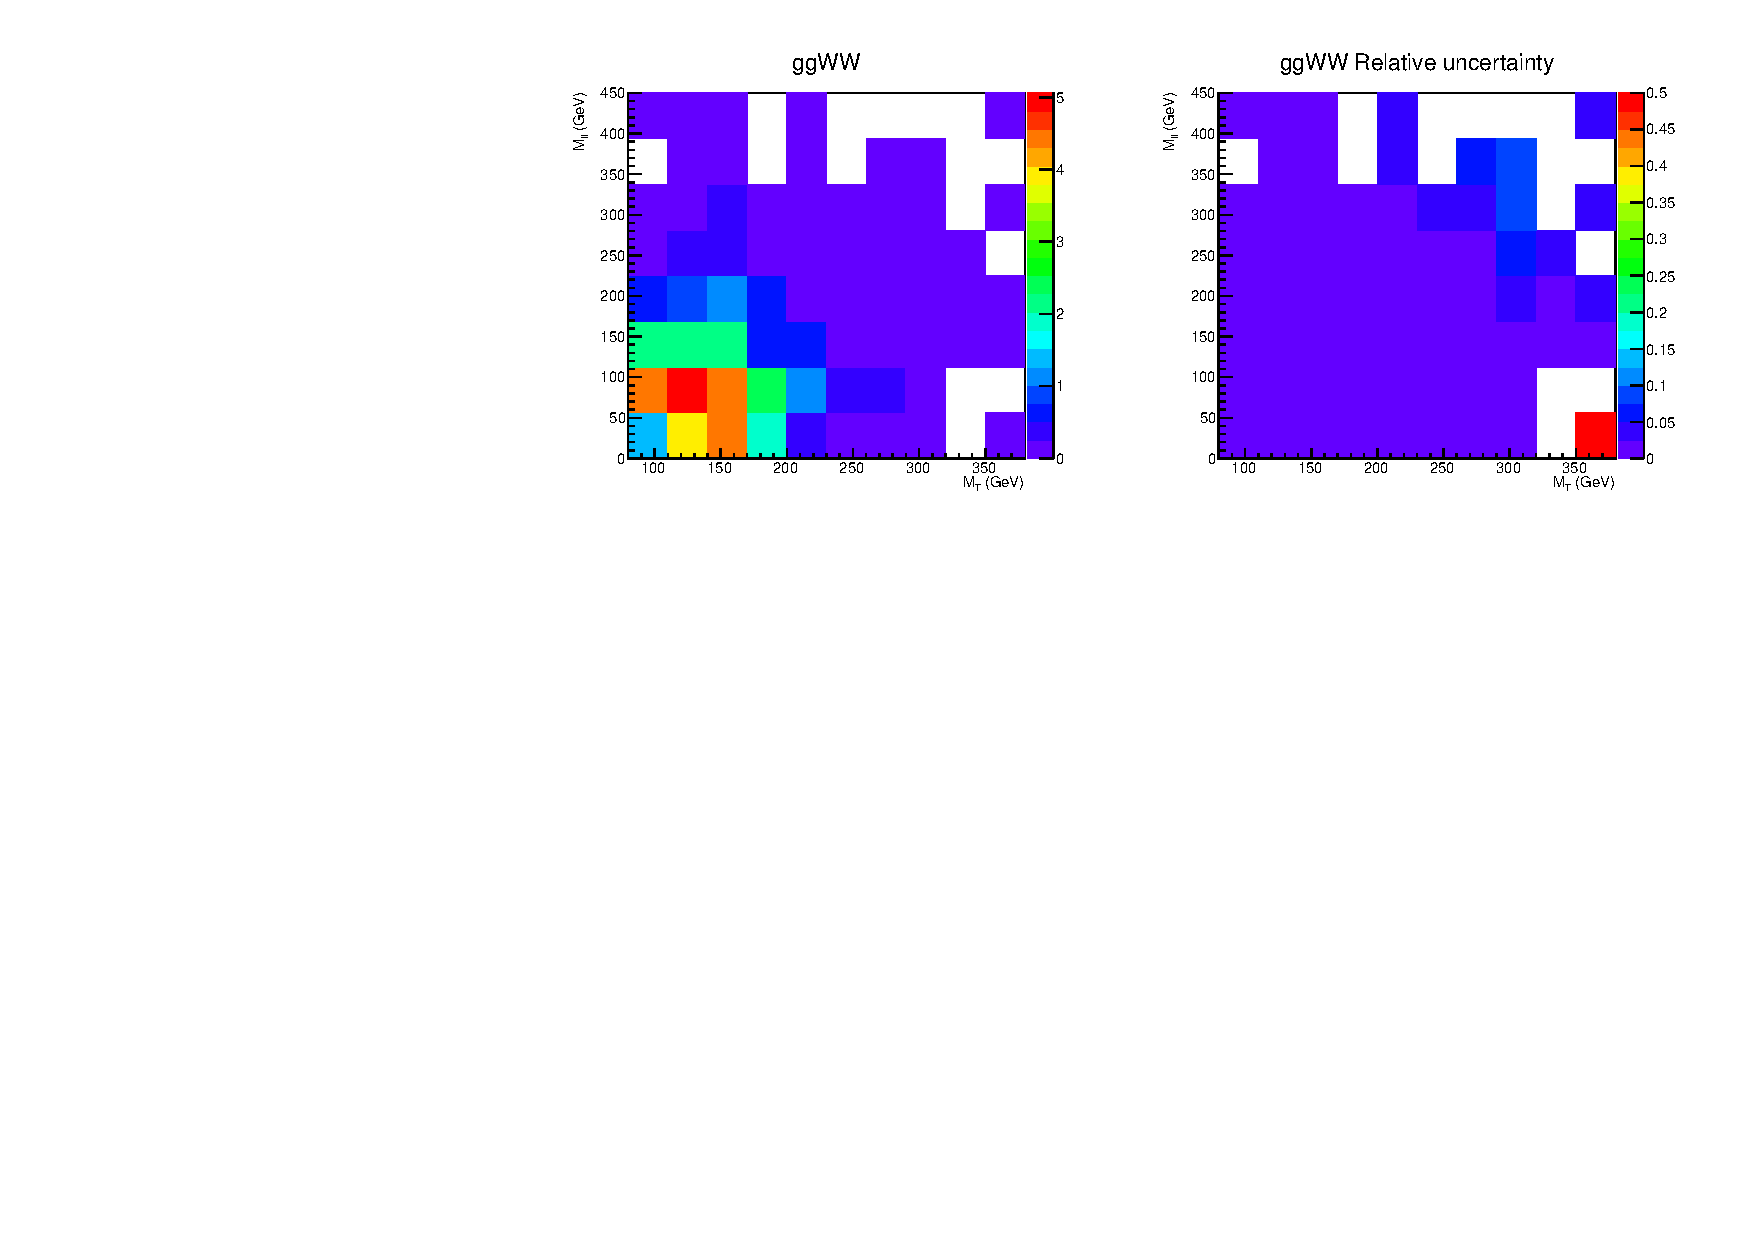
\includegraphics[width=0.8\textwidth]{figures/2dtemplate_ggWW_mH400_1j.pdf}
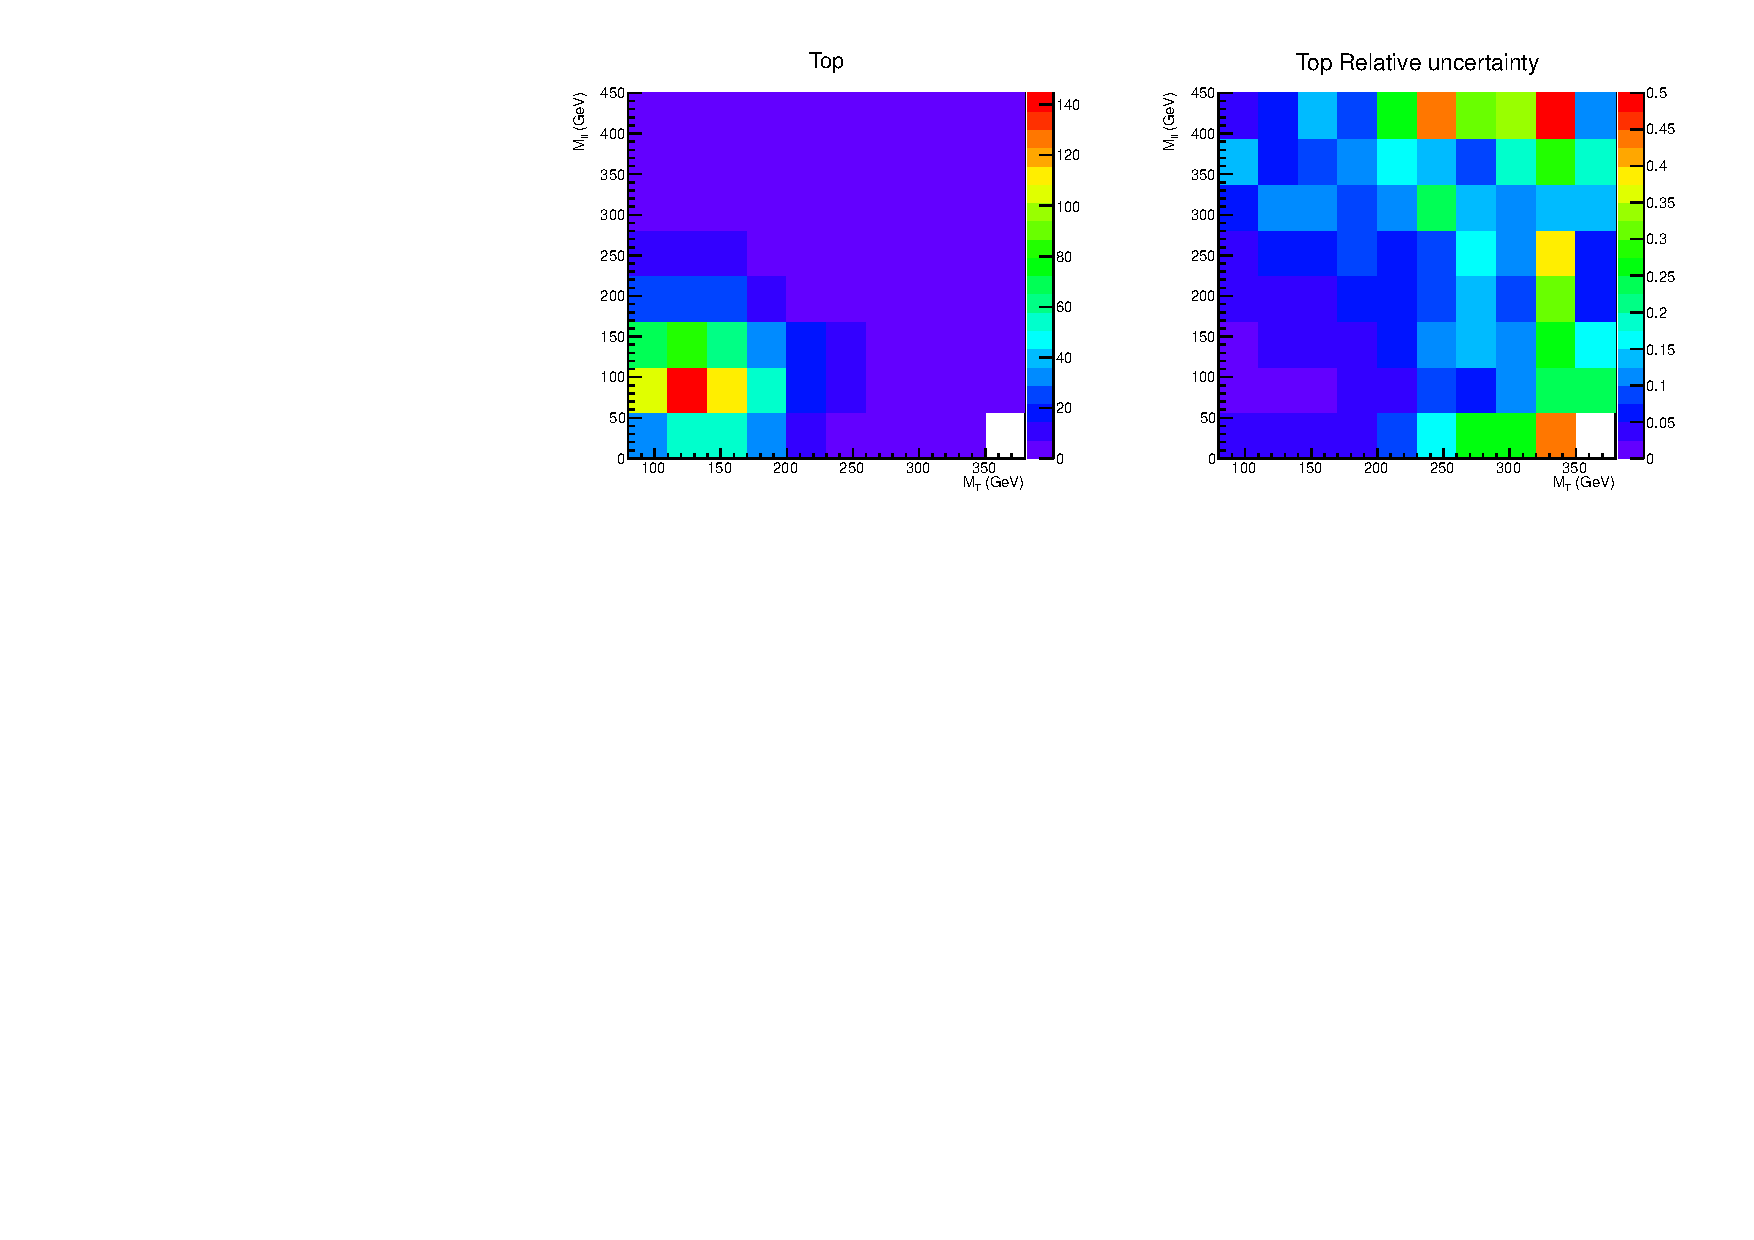
\includegraphics[width=0.8\textwidth]{figures/2dtemplate_Top_mH400_1j.pdf}
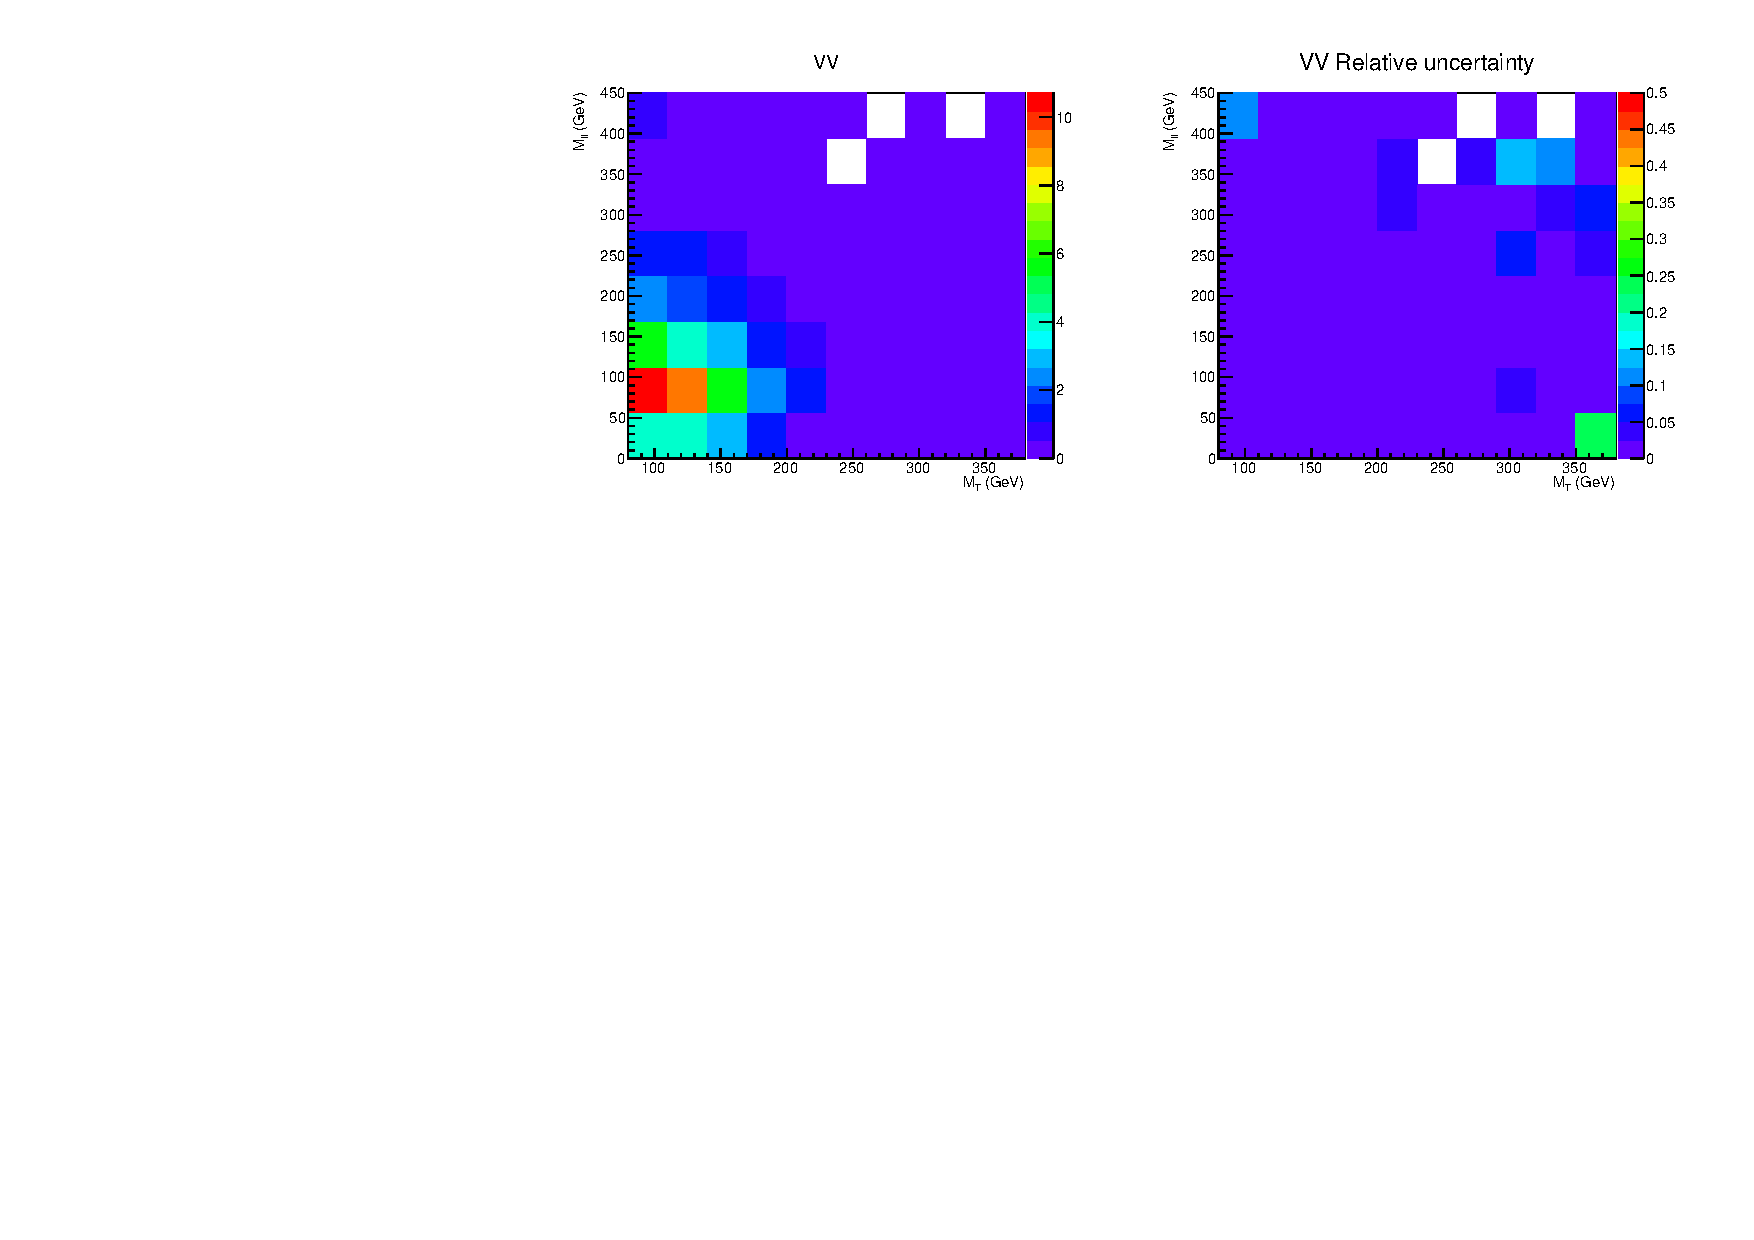
\includegraphics[width=0.8\textwidth]{figures/2dtemplate_VV_mH400_1j.pdf}
\caption{Templates(left) and relative statistical uncertainty of the MC sample(right) 
of \qqww, \ggww, \topbkg\ and \vv. 
The templates are for \mHi\ = 400 \GeV\ analysis in the 1-jet category.}
\label{fig:2dtemplate_400_1j_2}
\end{figure}

\begin{figure}[htp]
\centering
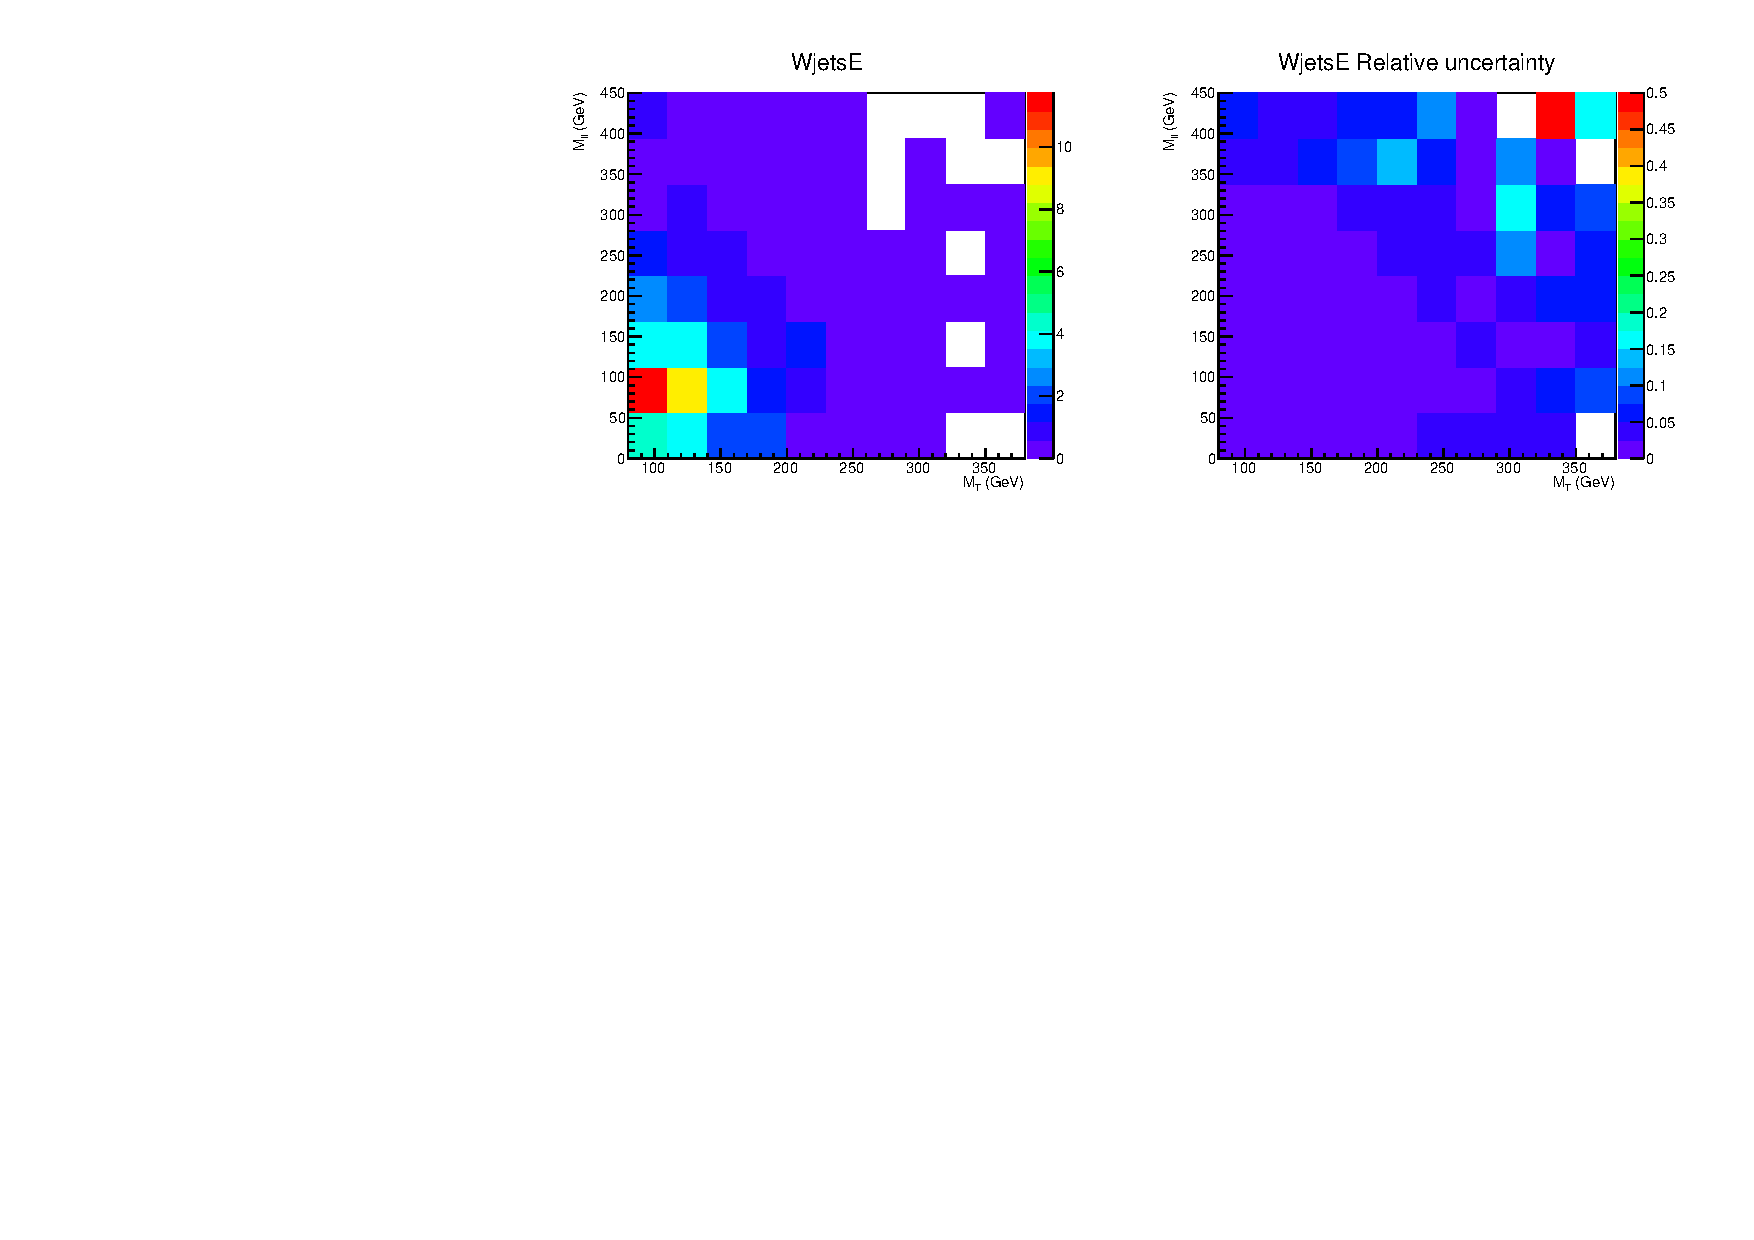
\includegraphics[width=0.8\textwidth]{figures/2dtemplate_WjetsE_mH400_1j.pdf}
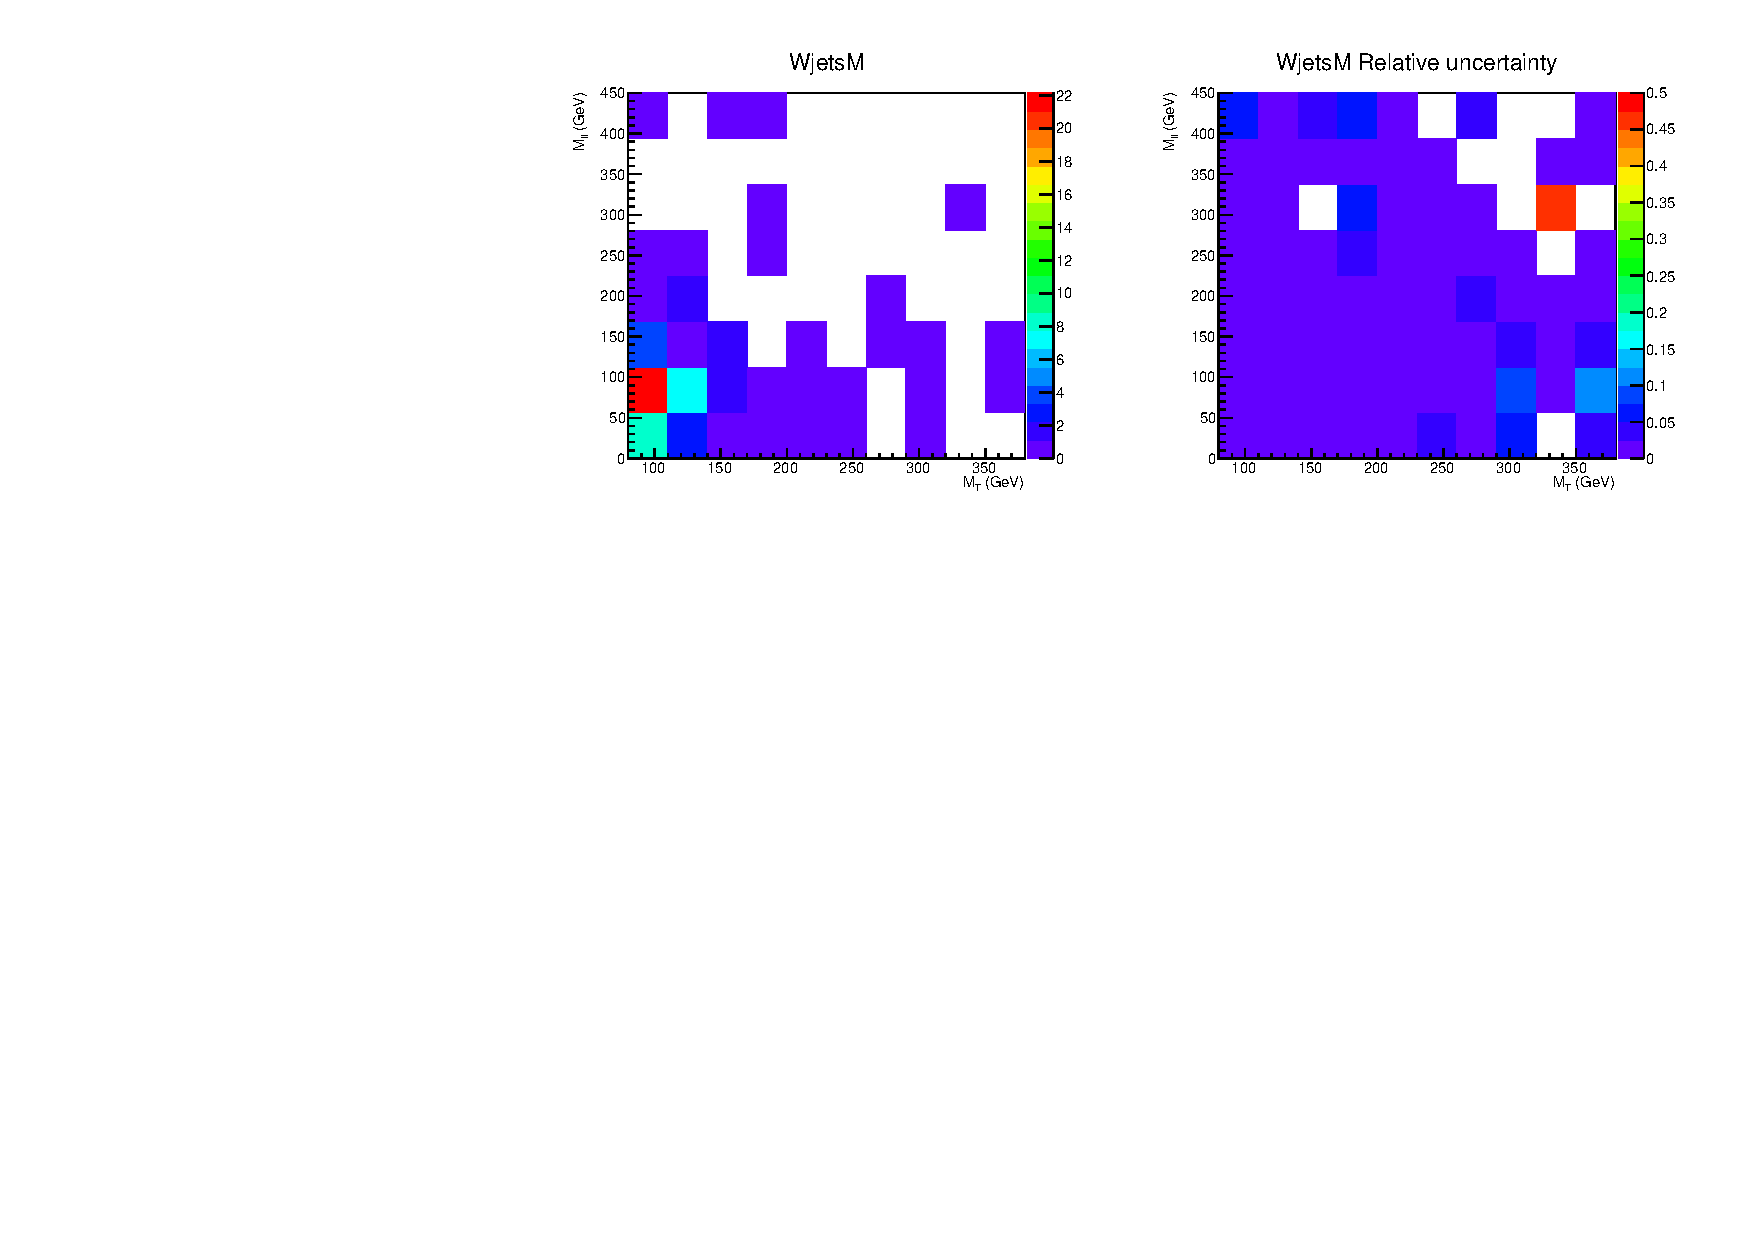
\includegraphics[width=0.8\textwidth]{figures/2dtemplate_WjetsM_mH400_1j.pdf}
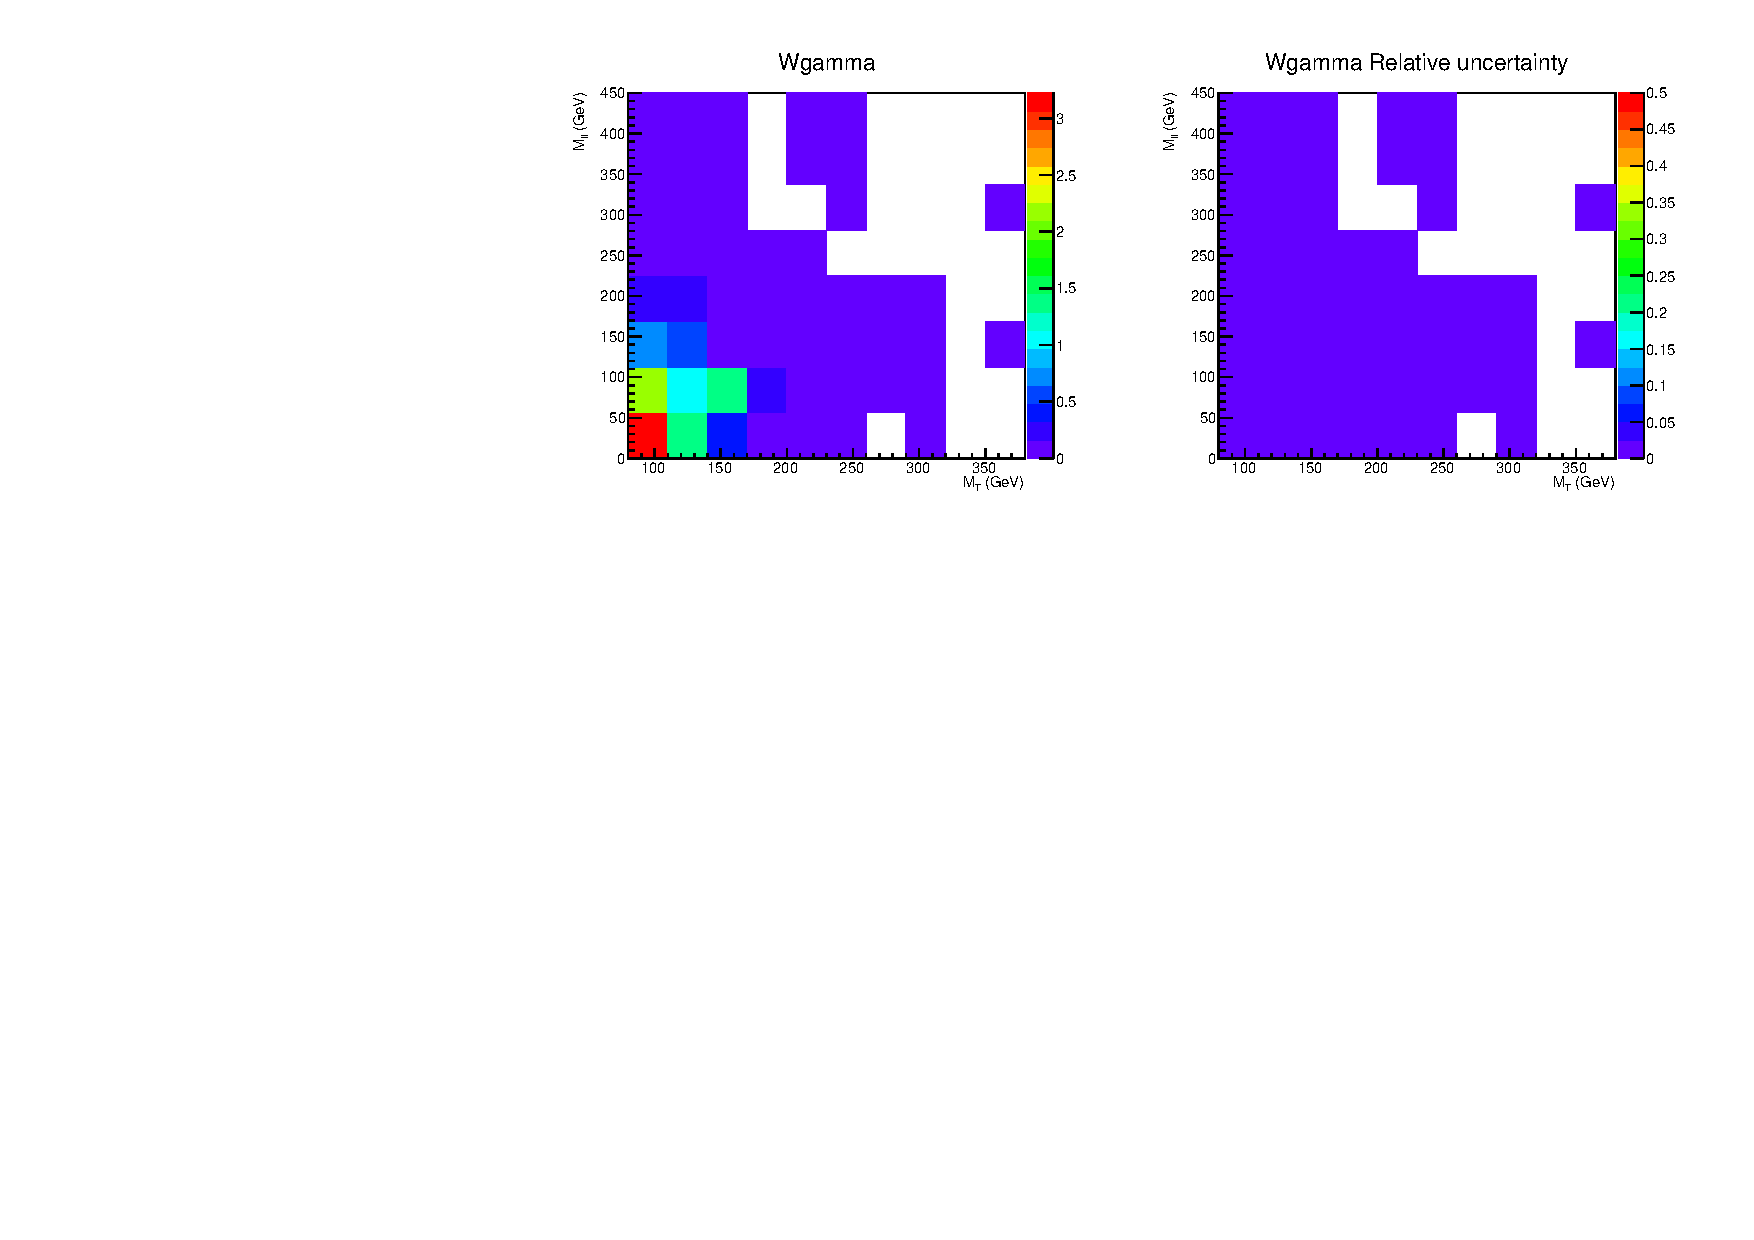
\includegraphics[width=0.8\textwidth]{figures/2dtemplate_Wgamma_mH400_1j.pdf}
\caption{Templates(left) and relative statistical uncertainty of the MC sample(right) 
of \WjetsE, \WjetsM\ and \wgamma. 
The templates are for \mHi\ = 400 \GeV\ analysis in the 1-jet category.}
\label{fig:2dtemplate_400_1j_3}
\end{figure}

\begin{figure}[htp]
\centering
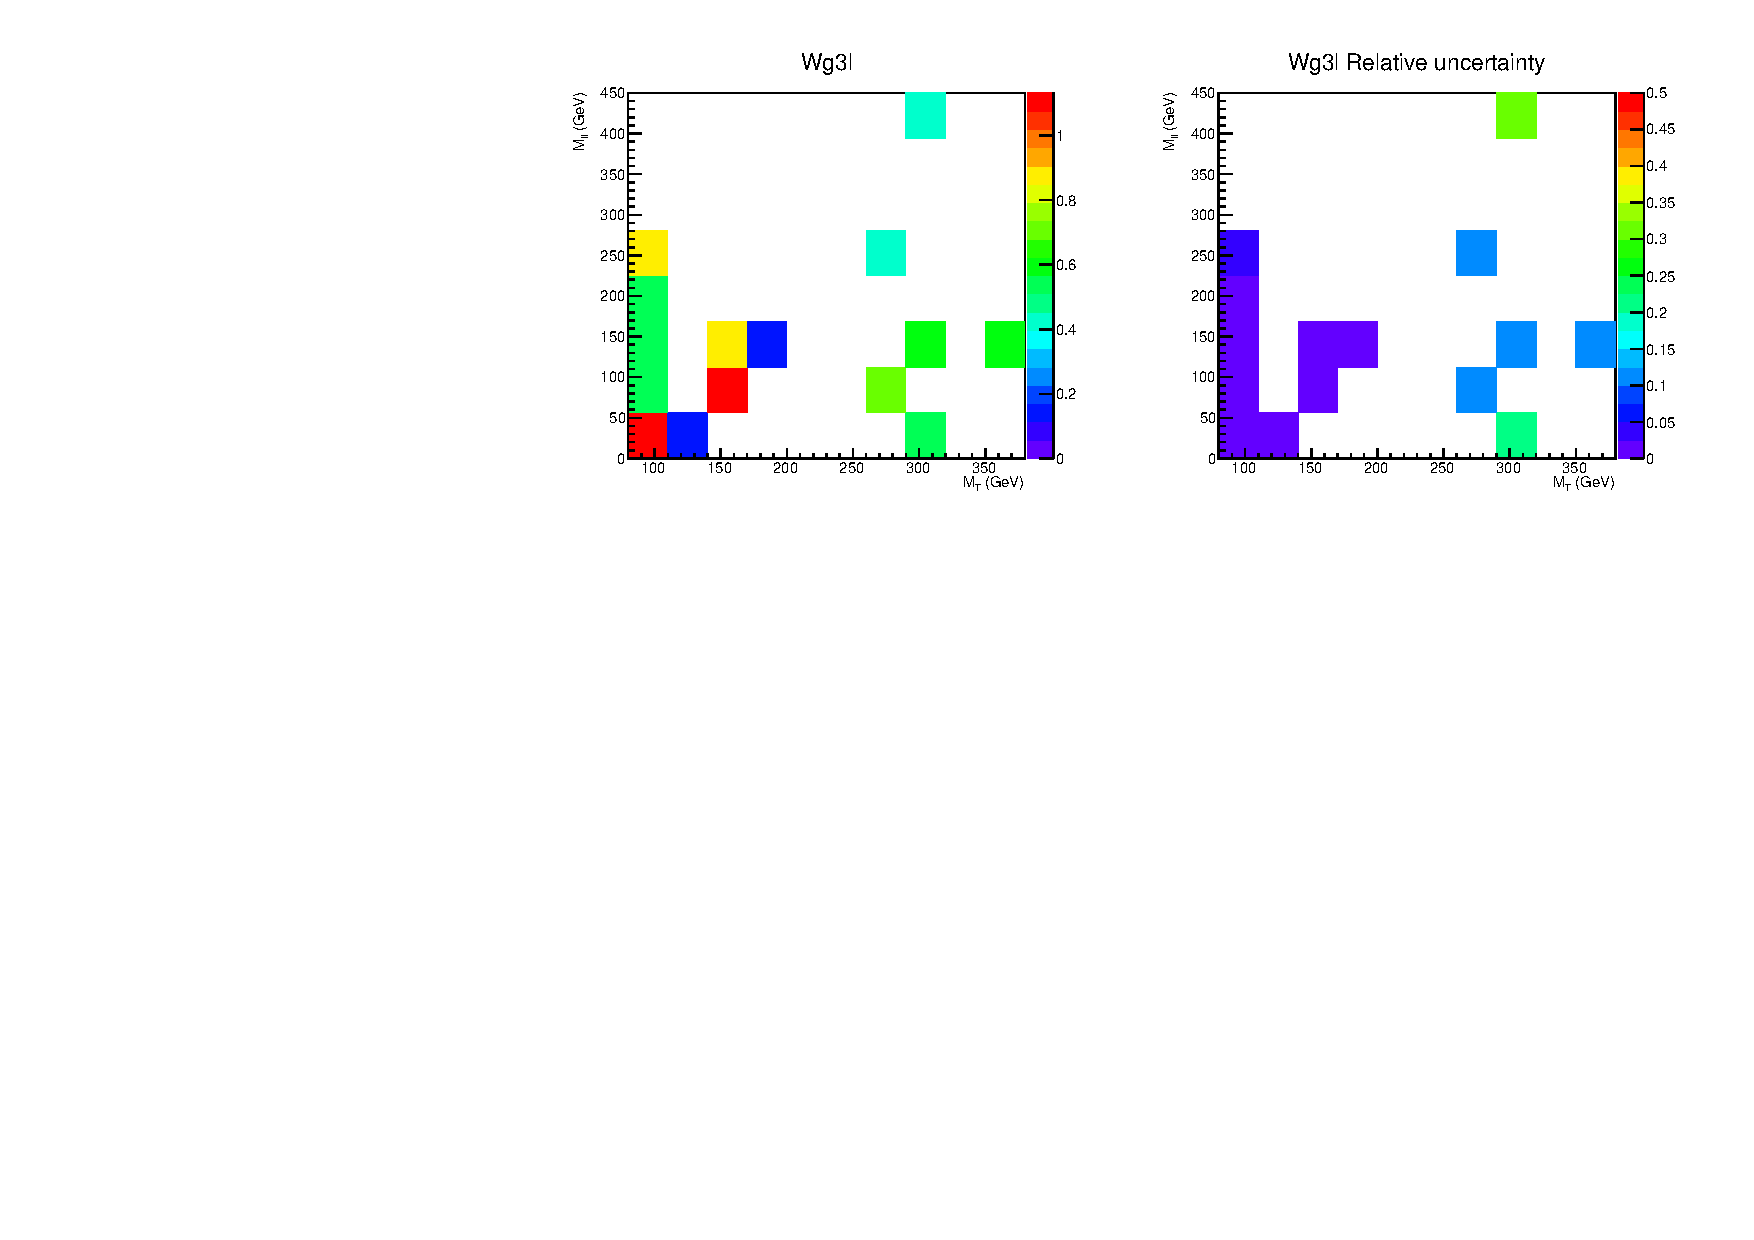
\includegraphics[width=0.8\textwidth]{figures/2dtemplate_Wg3l_mH400_1j.pdf}
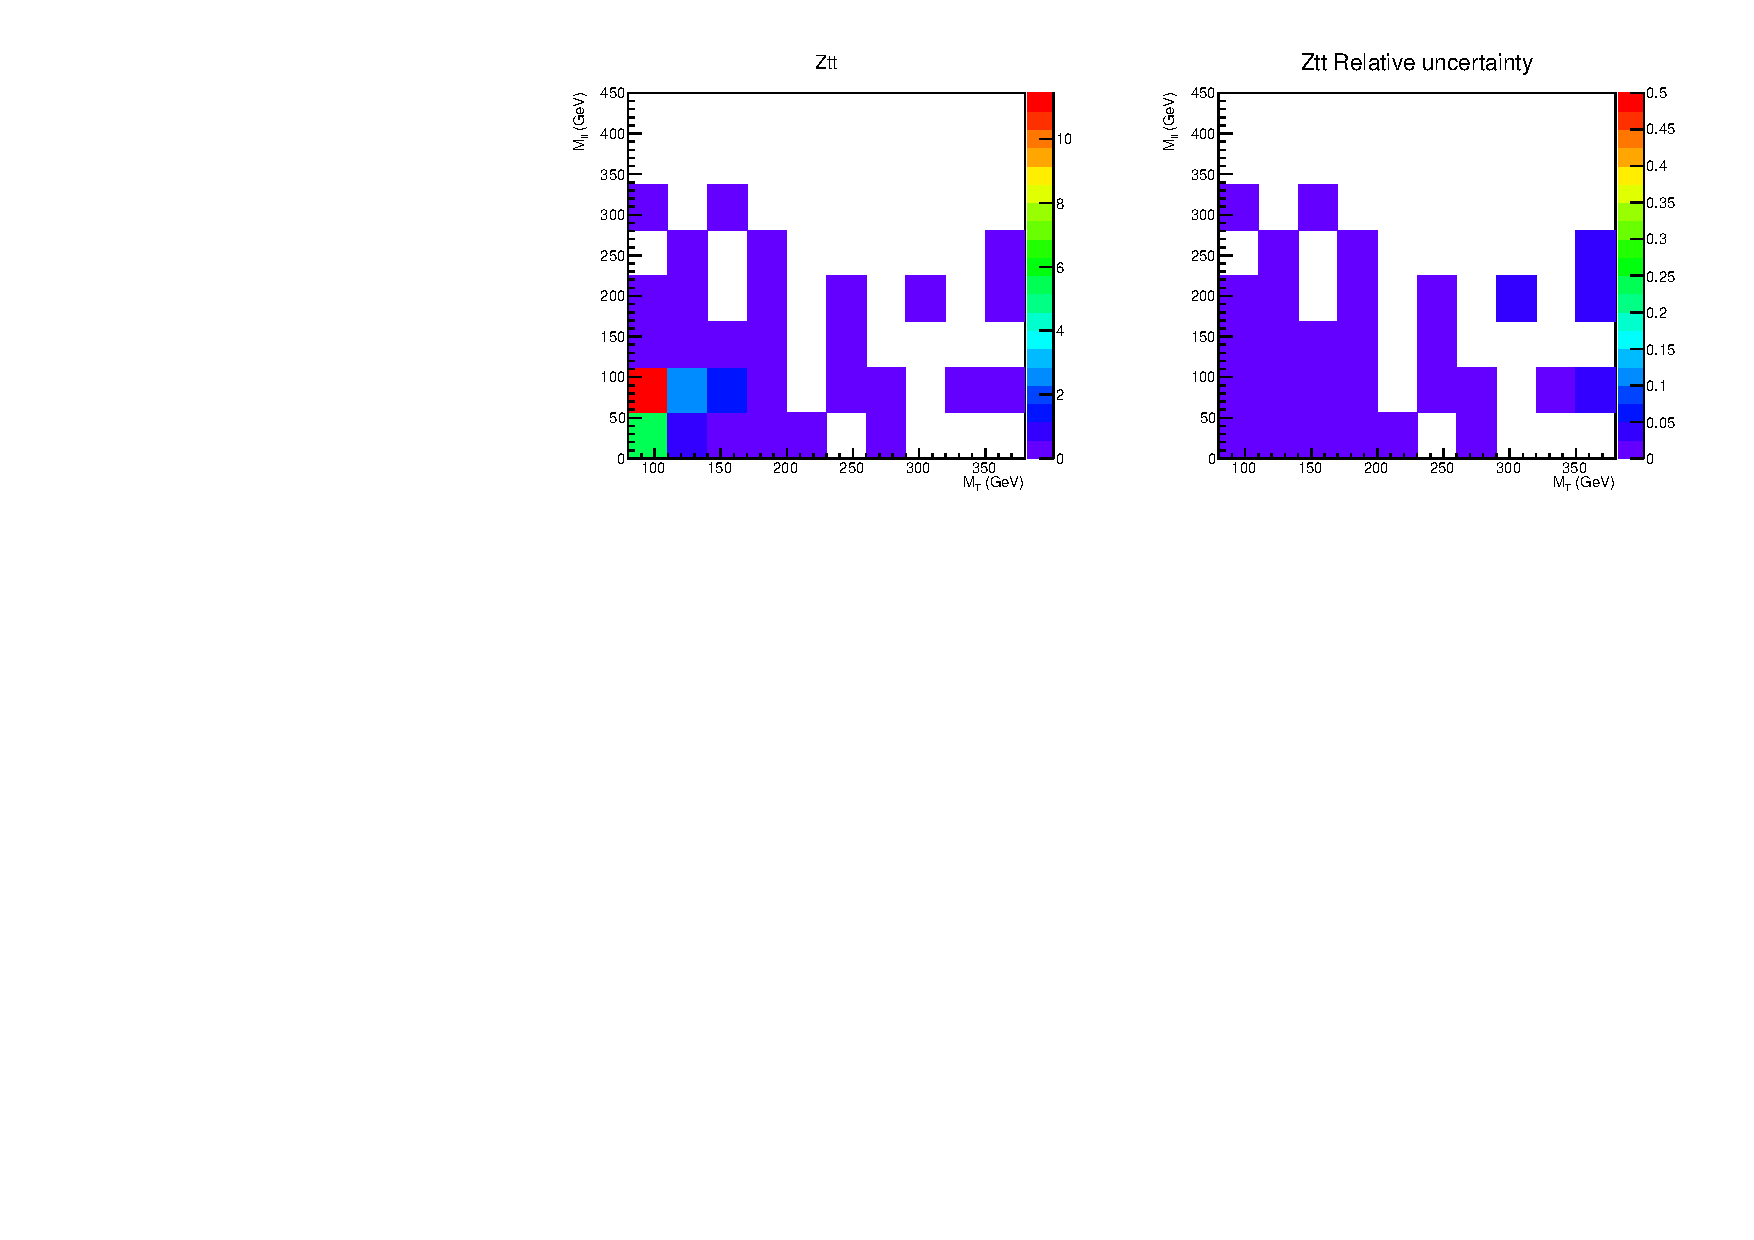
\includegraphics[width=0.8\textwidth]{figures/2dtemplate_Ztt_mH400_1j.pdf}
\caption{Templates(left) and relative statistical uncertainty of the MC sample(right) 
of \wgammastar\ and \ztt. 
The templates are for \mHi\ = 400 \GeV\ analysis in the 1-jet category.}
\label{fig:2dtemplate_400_1j_4}
\end{figure} 
